We implemented GSACO-O algorithm in Python using PyTorch, as it handles tensor operations efficiently and provides a multiprocessing library for
parallelization, thus significantly speeding up the ants' execution of the GS procedure in each GSACO-O iteration.%
\footnote{The source code is publicly available in our GitHub repository:
	\url{https://github.com/prosysscience/GSACO}}
The first challenge consists of determining suitable values for the input
parameters listed in Table~\ref{tab:parameters}, i.e.,
all parameters but the internally calculated pheromone level $\tau_e$ on edges~$e$.
We adhere to the parameters specified in Table~\ref{tab:p_value}, setting a time constraint~$l$ of $10$ minutes for objective makespan and $5$ minutes for objective operations. 
Setting different time limits for these two aspects allows the algorithm to tailor its computational efforts to the specific demands of each task. While makespan optimization seeks the best possible sequence over all operations (requiring extensive computation), optimizing operational efficiency focuses on making quicker adjustments that enhance day-to-day operations without the need for extensive computation. 
For the SMSP instances derived from the SMT2020 dataset, we consider up to $5$ operations per job for minimizing makespan and up to $15$ operations per job for optimizing operational throughput. These parameters are practical, given the stochastic nature of the problem which often necessitates frequent rescheduling. Additionally, we define a short planning horizon~$h$ to accommodate near-term scheduling requirements.
For the initial pheromone level~$\tau_y$,
we start from value~$1$, and take $0.00001$ as the minimum $\tau_z$
to avoid going down to $0$, considering that the GS procedure can only
select edges with non-zero entries in the pheromone matrix.
The values for the number~$k$ of ants, the evaporation rate~$\rho$,
and the pheromone contribution~$c$ are more sophisticated to pick.
That is, we tuned these parameters in a trial-and-error process that,
starting from a baseline, inspects deviations of the final makespan and convergence speed obtained with iterative modifications.
Certainly, an automated approach would be desirable to
perform this task efficiently for new instance sets.%
%
\begin{table}[t]
	\caption{GSACO input parameter values}\label{tab:p_value} \centering
	\begin{tabular}{|l|l|}
		\hline
		Parameter & Value \\ \hline
		$o$ & $makespan$/$operations$        \\
		$l$ & $10/5$        \\
		$n$ & $1$--$5$/$15$ \\
		$h$ & $1$--$6$ \\
		$k$ & $10$ \\
		$\tau_{y}$ & $1$ \\
		$\tau_{z}$ & $0.00001$ \\
		%		$\alpha$ & 1  \\
		%		$\beta$ & 1     \\
		$\rho$ & $0.7$ \\
		$c$ & $0.5$ \\
		\hline
	\end{tabular}
\end{table}

To evaluate large-scale SMSP instances,
we consider two semiconductor production scenarios of the SMT2020 dataset:
Low-Volume/High-Mix (LV/HM) and High-Volume/Low-Mix (HV/LM).
As indicated in Table~\ref{tab:Dataset},
both scenarios include more than $2000$ jobs and more than $1300$ machines,
modeling the production processes of modern semiconductor fabs.
The main difference is given by the number of products and associated production routes for jobs, where LV/HM considers $10$ production routes varying between
$200$--$600$ steps in total, while HV/LM comprises $2$ production routes with about
$300$ or $600$ steps, respectively.
Originally, the LV/HM and HV/LM scenarios have been designed to represent fab load at the
start of simulation runs, so that the jobs are at different steps of their
production routes.
We focus on scheduling for operations~$n$ from~$1$ up to~$5$,
to be performed per job.
Hence, the operations $O$ to schedule gradually increase from the
number $J$ of jobs, in case of the operations $n=1$,
% , given in Table~\ref{tab:Dataset},
to more than $10000$ operations % obtained
for the longest % planning 
horizon $n=5$.

\begin{table}[t]
	\caption{Number of jobs, machines, and operations for SMSP instances}\label{tab:Dataset} \centering
	\begin{tabular}{|l|c|c|c|}
		\hline
		Scenario & $J$    & $M$    & $O$              \\ \hline
		LV/HM    & $2156$ & $1313$ & up to $10747$    \\ 
		HV/LM    & $2256$ & $1443$ & up to $11218$    \\
		\hline
	\end{tabular}
\end{table}
%

\begin{table*}[t]
	\caption{SMSP results obtained with CP and GSACO \cite{Ali2024}}\label{tab:results} \centering
	\begin{tabular}{|l|l|l|l|l|l|l|l|l|l|l|l|}
		\hline
		&
		&
		\multicolumn{2}{c|}{$1$ min} &
		\multicolumn{2}{c|}{$3$ min} &
		\multicolumn{2}{c|}{$5$ min} &
		\multicolumn{2}{c|}{$7$ min} &
		\multicolumn{2}{c|}{$9$ min} \\ \cline{3-12} 
		$n$ & Scenario & CP & GSACO & CP & GSACO & CP & GSACO & CP & GSACO & CP & GSACO \\ \hline
		\multirow{2}{*}{$1$} & LV/HM & - & $3735$ & $18572$ & $3725$ & $3746$ & $3725$ & $3723$ & $3725$ & $3723$ & $3725$  \\
		& HV/LM & - & $1405$ & - & $1405$ & $2242$ & $1405$ & $1609$ & $1405$ & $1600$ & $1405$ \\
		\multirow{2}{*}{$2$} & LV/HM & - & $3773$ & - & $3751$ & - & $3750$ & - & $3739$ & $4398$ & $3739$ \\
		& HV/LM & - & $1653$ & - & $1644$ & - & $1611$ & - & $1611$ & - & $1611$   \\
		\multirow{2}{*}{$3$} & LV/HM & - & $3880$ & - & $3867$ & - & $3836$ & - & $3834$ & - & $3834$   \\
		& HV/LM & - & $1902$ & - & $1889$ & - & $1889$ & - & $1876$ & - & $1876$     \\
		\multirow{2}{*}{$4$} & LV/HM & - & $4578$ & - & $4540$ & - & $4540$ & - & $4540$ & - & $4540$     \\
		& HV/LM & - & $2207$ & - & $2113$ & - & $2113$ & - & $2093$ & - & $2093$  \\
		\multirow{2}{*}{$5$} & LV/HM & - & $4680$ & - & $4680$ & - & $4553$ & - & $4553$ & - & $4553$   \\	
		& HV/LM & - & $2667$ & - & $2566$ & - & $2566$ & - & $2518$ & - & $2518$ \\
		\hline  
	\end{tabular}
\end{table*}

While running with a time limit $l$ of $10$ minutes,
Table~\ref{tab:results} reports the makespans of current best schedules
found by the CP solver OR-Tools and our GSACO implementation
at $1$, $3$, $5$, $7$, and $9$ minutes of computing time.
Considering that the SMSP instances are large,
OR-Tools now takes $3$ minutes to come up with the first solution(s)
for the shortest planning horizon $n=1$ on the LV/HM scenario.
Within the same fraction of computing time, GSACO-O already converges to a
makespan of $3725$ and then proceeds with iterations that do not
yield further improvements.
That the best schedule found by GSACO is not optimal is witnessed by a
marginally better solution obtained by OR-Tools after $7$ minutes.
However, for the other SMSP instances, OR-Tools is unable to improve over
GSACO within $9$ minutes, and it cannot even provide feasible schedules
for planning horizons from $n=2$ on the HV/LM scenario or $n=3$ 
on LV/HM.
We performed our experiments on a TUXEDO Pulse 14 Gen1 machine
equipped with an 8-core AMD Ryzen 7 4800H processor at 2.9GHz and onboard
Radeon graphics card.

\begin{figure*}[t]
	\centering
	\begin{subfigure}[b]{0.45\linewidth}
		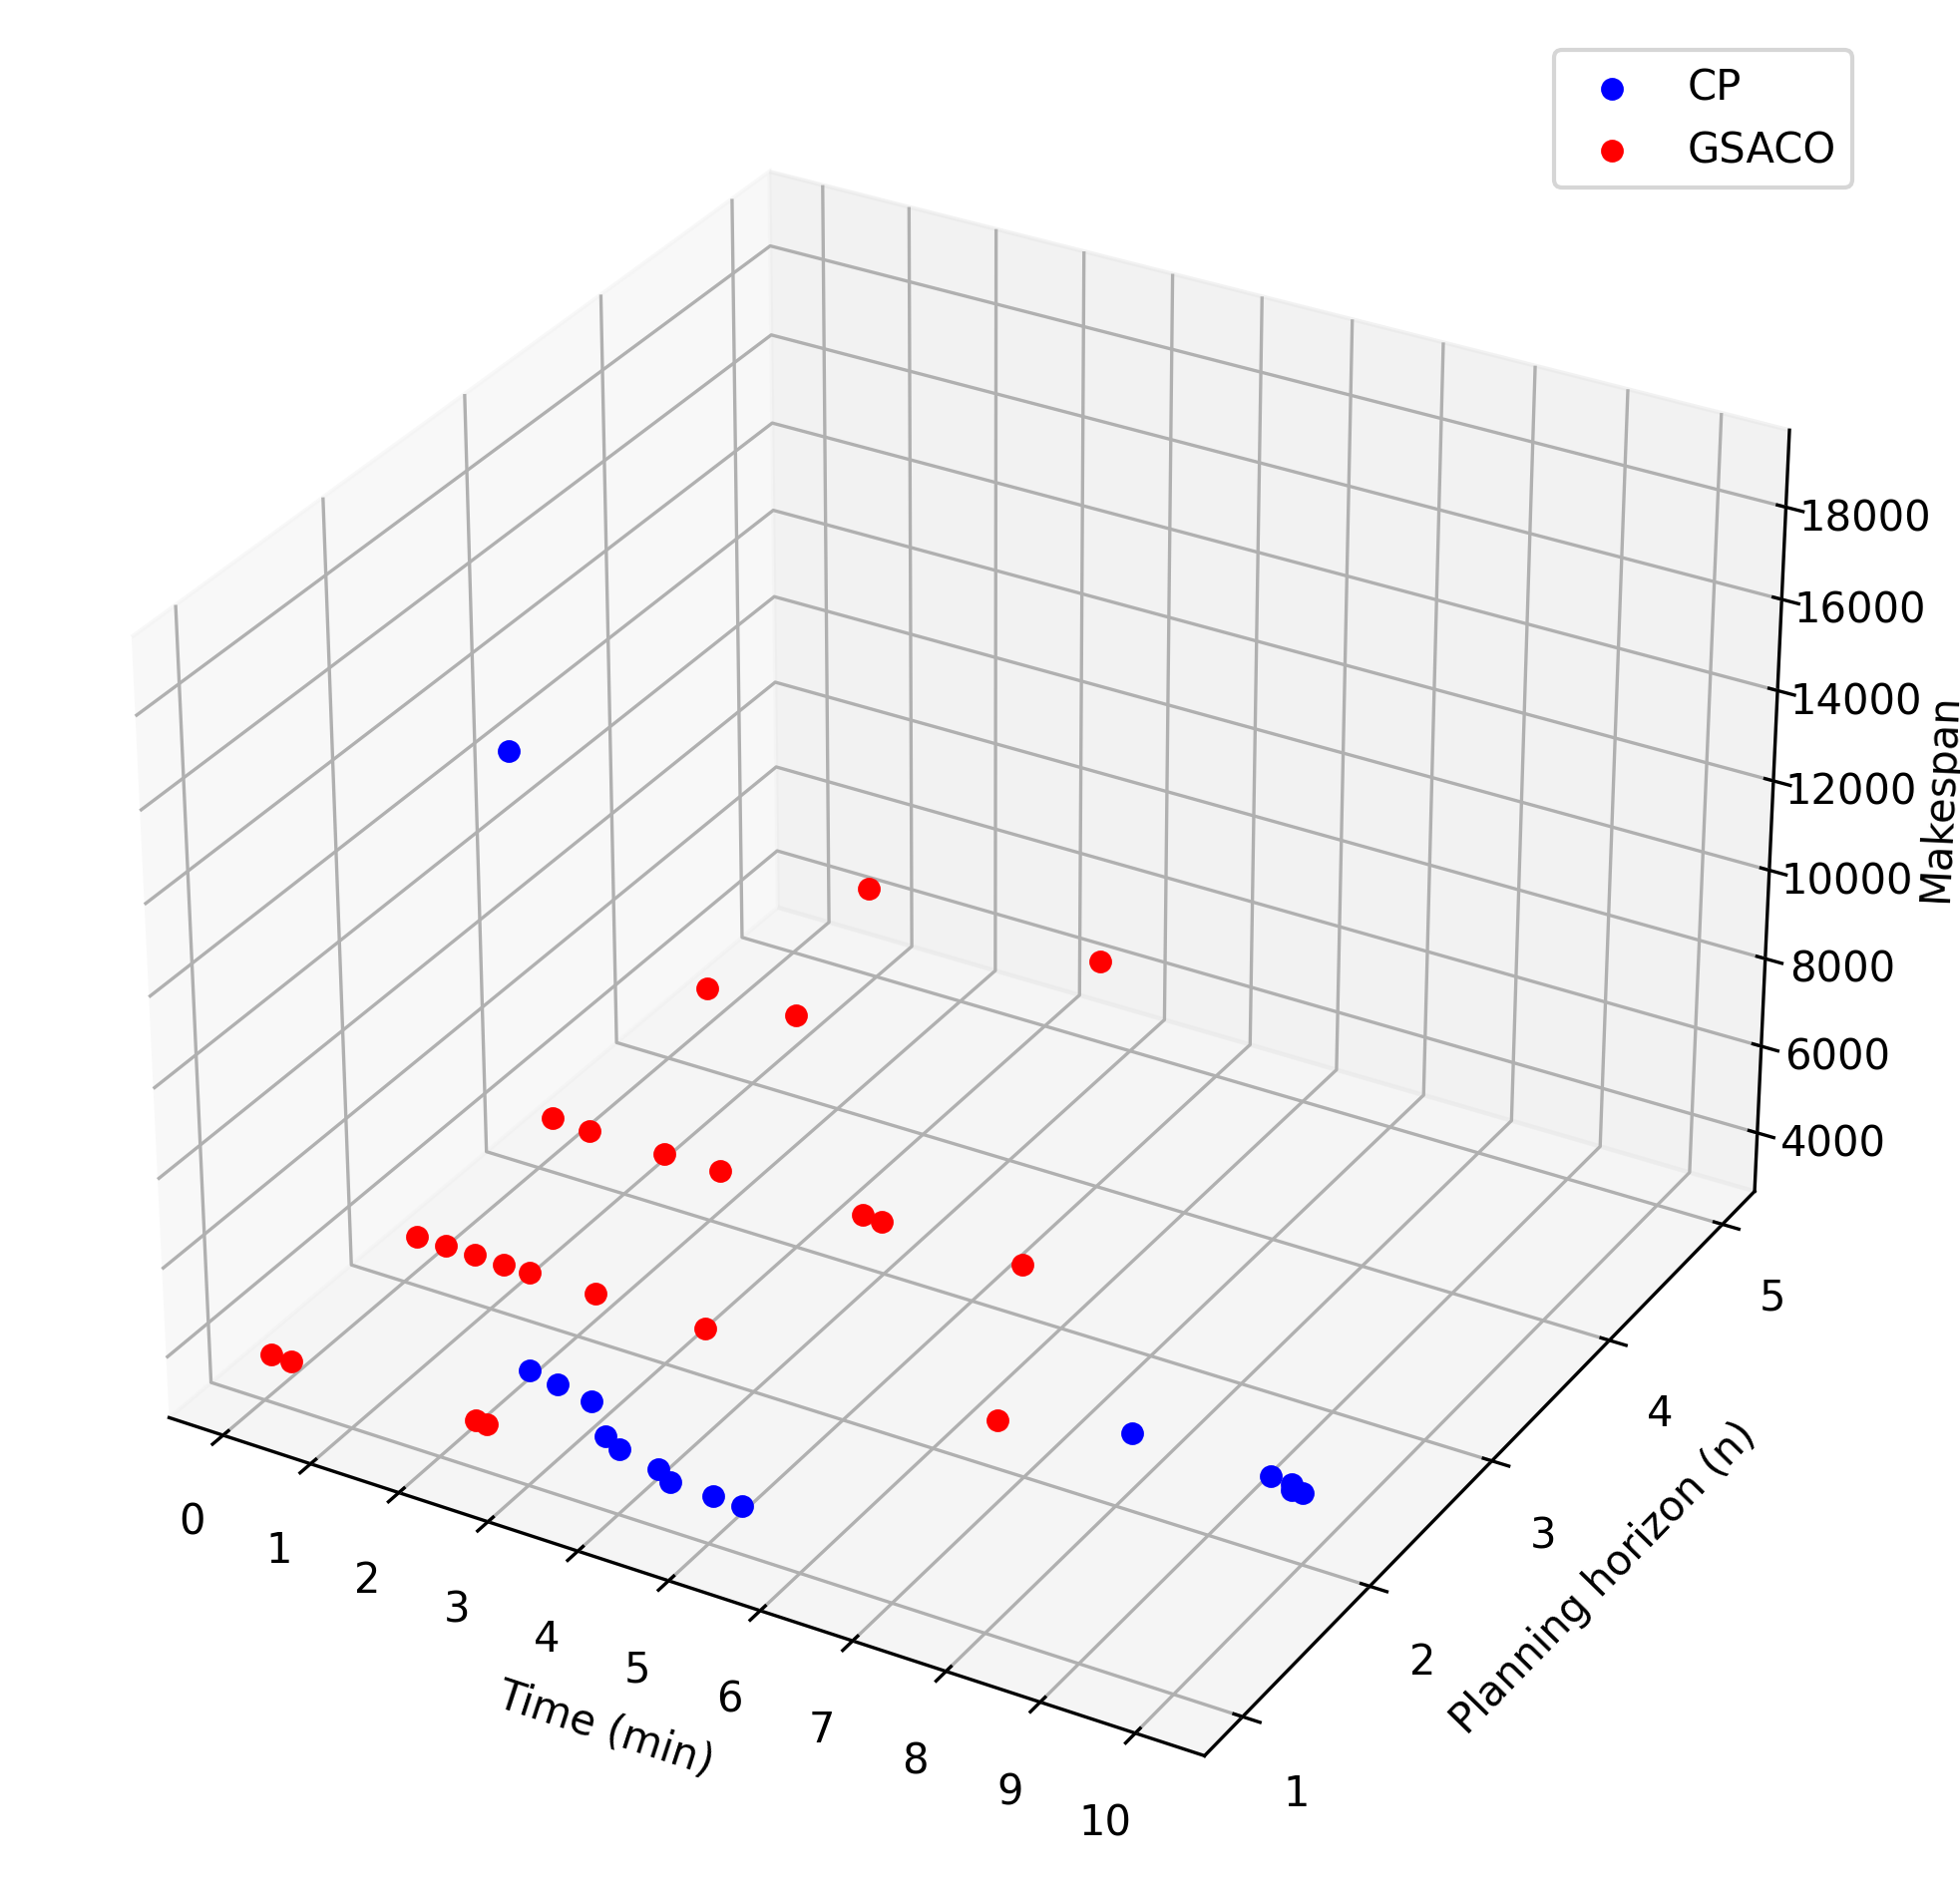
\includegraphics[width=\textwidth]{LVHM.png}
		\caption{LV/HM scenario}
		\label{subfig:l}
	\end{subfigure}
	\hfill
	\begin{subfigure}[b]{0.45\linewidth}
		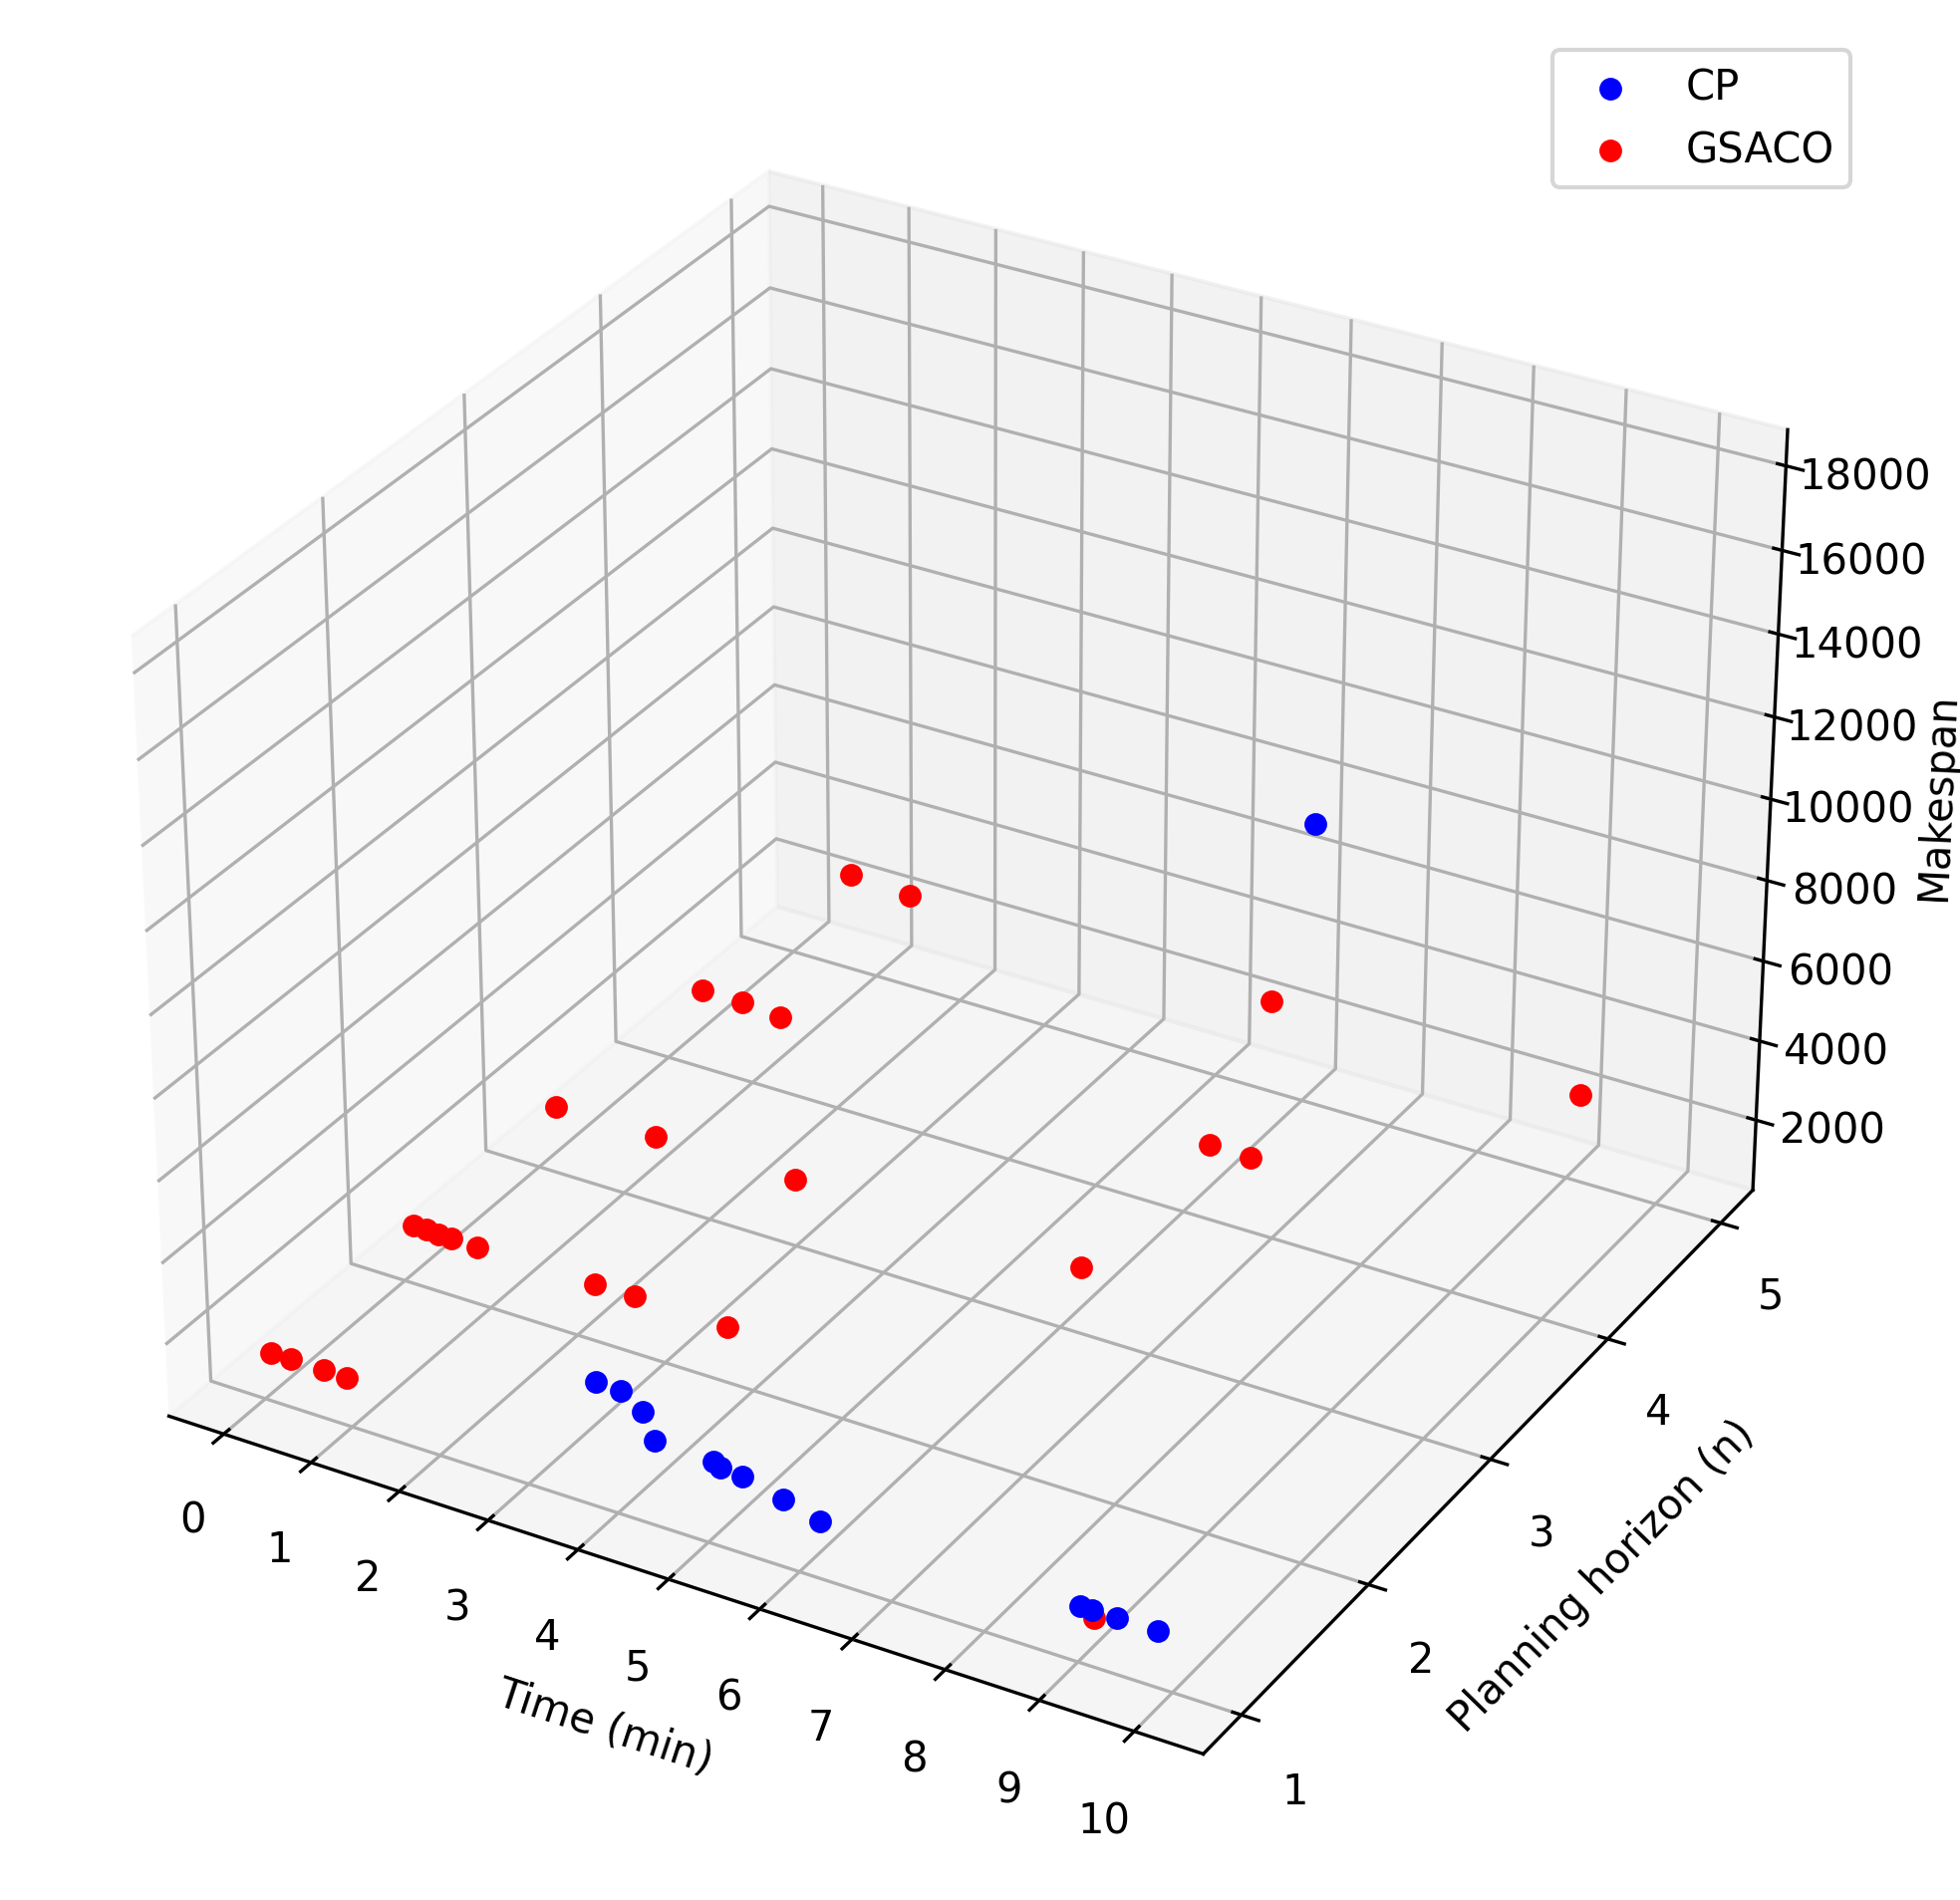
\includegraphics[width=\textwidth]{HVLM.png}
		\caption{HV/LM scenario}
		\label{subfig:h}
	\end{subfigure}
	\caption{Makespan improvements of schedules for SMSP instances obtained with CP and GSACO \cite{Ali2024}\label{fig:makespan}}
\end{figure*}

The quick convergence of our GSACO implementation is also outlined by the makespan improvements plotted in Figure~\ref{fig:makespan}.
On the LV/HM scenario displayed in Figure~\ref{subfig:l}, 
GSACO obtains its best schedules within $7$ minutes
for all planning horizons.
Only for the longest planning horizon $n=5$
on the HV/LM scenario in Figure~\ref{subfig:h},
an improvement occurs after more than the $9$ minutes of computing time
listed in the rightmost column of Table~\ref{tab:results}.
Comparing the SMSP instances for which OR-Tools manages to provide
feasible schedules,
the convergence to makespans in roughly the range of GSACO's results
takes significantly more computing time.
Hence, the time limit that would be necessary to break even with GSACO,
as accomplished within $7$ minutes for the shortest planning horizon
$n=1$ on the LV/HM scenario,
cannot be predicted for the SMSP instances with longer planning horizons.
Moreover, we observe that the initial schedules obtained 
in the first GSACO iteration by some of the ants running in parallel are of relatively high quality, while
OR-Tools sometimes finds outliers as its first solutions.
This phenomenon occurs for the planning horizons $n=1$ and $n=2$
on the LV/HM or HV/LM scenario, respectively, where the latter
schedule of makespan $17664$ is found after more than $9$ minutes
and thus not listed in Table~\ref{tab:results}.


\begin{table}[t]
	\caption{Percentage Change in Dispatcher Performance Over Planning Hours LV/HM}
	\label{tab:dispatchers-LVHM}
	\begin{tabular}{|c|lcllllll|ll|}
		\hline
		\multirow{3}{*}{\begin{tabular}[c]{@{}c@{}}Planning \\ horizon\end{tabular}} &
		\multicolumn{8}{c|}{Dispatcher} &
		\multicolumn{2}{c|}{Scheduler} \\ \cline{2-11} 
		&
		\multicolumn{2}{c|}{FIFO} &
		\multicolumn{2}{c|}{CR} &
		\multicolumn{2}{c|}{RANDOM} &
		\multicolumn{2}{c|}{GSACO-O} &
		\multicolumn{2}{c|}{GSACO-O} \\ \cline{2-11} 
		&
		\multicolumn{1}{l|}{Ops/Lots} &
		\multicolumn{1}{l|}{Change} &
		\multicolumn{1}{l|}{Ops/Lots} &
		\multicolumn{1}{l|}{Change} &
		\multicolumn{1}{l|}{Ops/Lots} &
		\multicolumn{1}{l|}{Change} &
		\multicolumn{1}{l|}{Ops/Lots} &
		Change &
		\multicolumn{1}{l|}{Ops/Lots} &
		Change \\ \hline
		1 &
		\multicolumn{1}{l|}{1419/0} &
		\multicolumn{1}{c|}{-} &
		\multicolumn{1}{l|}{1416/0} &
		\multicolumn{1}{l|}{-0.21\%} &
		\multicolumn{1}{l|}{1403/0} &
		\multicolumn{1}{l|}{-1.12\%} &
		\multicolumn{1}{l|}{1442//0} &
		1.62\% &
		\multicolumn{1}{l|}{1422} &
		0.21\% \\
		2 &
		\multicolumn{1}{l|}{2249/0} &
		\multicolumn{1}{c|}{-} &
		\multicolumn{1}{l|}{2328/0} &
		\multicolumn{1}{l|}{3.51\%} &
		\multicolumn{1}{l|}{2275/0} &
		\multicolumn{1}{l|}{1.15\%} &
		\multicolumn{1}{l|}{2409/0} &
		7.11\% &
		\multicolumn{1}{l|}{2368} &
		5.29\% \\
		3 &
		\multicolumn{1}{l|}{2384/0} &
		\multicolumn{1}{c|}{-} &
		\multicolumn{1}{l|}{3372/0} &
		\multicolumn{1}{l|}{2.67\%} &
		\multicolumn{1}{l|}{3314/0} &
		\multicolumn{1}{l|}{0.91\%} &
		\multicolumn{1}{l|}{3427/0} &
		4.35\% &
		\multicolumn{1}{l|}{3234} &
		-1.52\% \\
		4 &
		\multicolumn{1}{l|}{4018/1} &
		\multicolumn{1}{c|}{-} &
		\multicolumn{1}{l|}{4083/1} &
		\multicolumn{1}{l|}{1.61\%} &
		\multicolumn{1}{l|}{4039/1} &
		\multicolumn{1}{l|}{0.52\%} &
		\multicolumn{1}{l|}{4272/1} &
		6.32\% &
		\multicolumn{1}{l|}{4015} &
		-0.07\% \\
		5 &
		\multicolumn{1}{l|}{4901/1} &
		\multicolumn{1}{c|}{-} &
		\multicolumn{1}{l|}{5023/1} &
		\multicolumn{1}{l|}{2.48\%} &
		\multicolumn{1}{l|}{4972/1} &
		\multicolumn{1}{l|}{1.44\%} &
		\multicolumn{1}{l|}{5174/2} &
		5.57\% &
		\multicolumn{1}{l|}{4722} &
		-3.65\% \\
		6 &
		\multicolumn{1}{l|}{5665/4} &
		\multicolumn{1}{c|}{-} &
		\multicolumn{1}{l|}{5799/3} &
		\multicolumn{1}{l|}{2.36\%} &
		\multicolumn{1}{l|}{5767/1} &
		\multicolumn{1}{l|}{1.80\%} &
		\multicolumn{1}{l|}{6014/2} &
		6.16\% &
		\multicolumn{1}{l|}{5306} &
		-6.33\% \\ \hline
	\end{tabular}%
\end{table}

\begin{table}[t]
	\caption{Percentage Change in Dispatcher Performance Over Planning Hours HV/LM}
	\label{tab:dispatchers-HVLM}
	\begin{tabular}{|c|lcllllll|ll|}
		\hline
		\multirow{3}{*}{\begin{tabular}[c]{@{}c@{}}Planning \\ horizon\end{tabular}} &
		\multicolumn{8}{c|}{Disaptcher} &
		\multicolumn{2}{c|}{Scheduler} \\ \cline{2-11} 
		&
		\multicolumn{2}{c|}{FIFO} &
		\multicolumn{2}{c|}{CR} &
		\multicolumn{2}{c|}{RANDOM} &
		\multicolumn{2}{c|}{GSACO-O} &
		\multicolumn{2}{c|}{GSACO-O} \\ \cline{2-11} 
		&
		\multicolumn{1}{l|}{Ops/Lots} &
		\multicolumn{1}{l|}{Change} &
		\multicolumn{1}{l|}{Ops/Lots} &
		\multicolumn{1}{l|}{Change} &
		\multicolumn{1}{l|}{Ops/Lots} &
		\multicolumn{1}{l|}{Change} &
		\multicolumn{1}{l|}{Ops/Lots} &
		Change &
		\multicolumn{1}{l|}{Ops/Lots} &
		Change \\ \hline
		1 &
		\multicolumn{1}{l|}{1821/0} &
		\multicolumn{1}{c|}{-} &
		\multicolumn{1}{l|}{1798/0} &
		\multicolumn{1}{l|}{-1.26\%} &
		\multicolumn{1}{l|}{1810/0} &
		\multicolumn{1}{l|}{-0.60\%} &
		\multicolumn{1}{l|}{1831/0} &
		0.54\% &
		\multicolumn{1}{l|}{1848/0} &
		1.48\% \\
		2 &
		\multicolumn{1}{l|}{2831/0} &
		\multicolumn{1}{c|}{-} &
		\multicolumn{1}{l|}{2811/0} &
		\multicolumn{1}{l|}{-0.71\%} &
		\multicolumn{1}{l|}{2852/0} &
		\multicolumn{1}{l|}{0.74\%} &
		\multicolumn{1}{l|}{2957/0} &
		4.45\% &
		\multicolumn{1}{l|}{2960/0} &
		4.55\% \\
		3 &
		\multicolumn{1}{l|}{4020/1} &
		\multicolumn{1}{c|}{-} &
		\multicolumn{1}{l|}{4021/1} &
		\multicolumn{1}{l|}{0.02\%} &
		\multicolumn{1}{l|}{4065/1} &
		\multicolumn{1}{l|}{1.12\%} &
		\multicolumn{1}{l|}{4162/1} &
		3.53\% &
		\multicolumn{1}{l|}{4093/1} &
		1.81\% \\
		4 &
		\multicolumn{1}{l|}{4914/4} &
		\multicolumn{1}{c|}{-} &
		\multicolumn{1}{l|}{4934/3} &
		\multicolumn{1}{l|}{0.40\%} &
		\multicolumn{1}{l|}{4975/3} &
		\multicolumn{1}{l|}{1.24\%} &
		\multicolumn{1}{l|}{5118/3} &
		4.15\% &
		\multicolumn{1}{l|}{4970/3} &
		1.07\% \\
		5 &
		\multicolumn{1}{l|}{5960/6} &
		\multicolumn{1}{c|}{-} &
		\multicolumn{1}{l|}{6003/5} &
		\multicolumn{1}{l|}{0.72\%} &
		\multicolumn{1}{l|}{6026/5} &
		\multicolumn{1}{l|}{1.10\%} &
		\multicolumn{1}{l|}{6263/5} &
		5.08\% &
		\multicolumn{1}{l|}{5975/5} &
		0.25\% \\
		6 &
		\multicolumn{1}{l|}{6841/8} &
		\multicolumn{1}{c|}{-} &
		\multicolumn{1}{l|}{6946/8} &
		\multicolumn{1}{l|}{1.53\%} &
		\multicolumn{1}{l|}{6973/9} &
		\multicolumn{1}{l|}{1.92\%} &
		\multicolumn{1}{l|}{7162/7} &
		4.69\% &
		\multicolumn{1}{l|}{6716/7} &
		-1.82\% \\ \hline
	\end{tabular}%
\end{table}

explain here

\begin{figure}[t]
	\centering
	\begin{subfigure}{0.32\textwidth}
		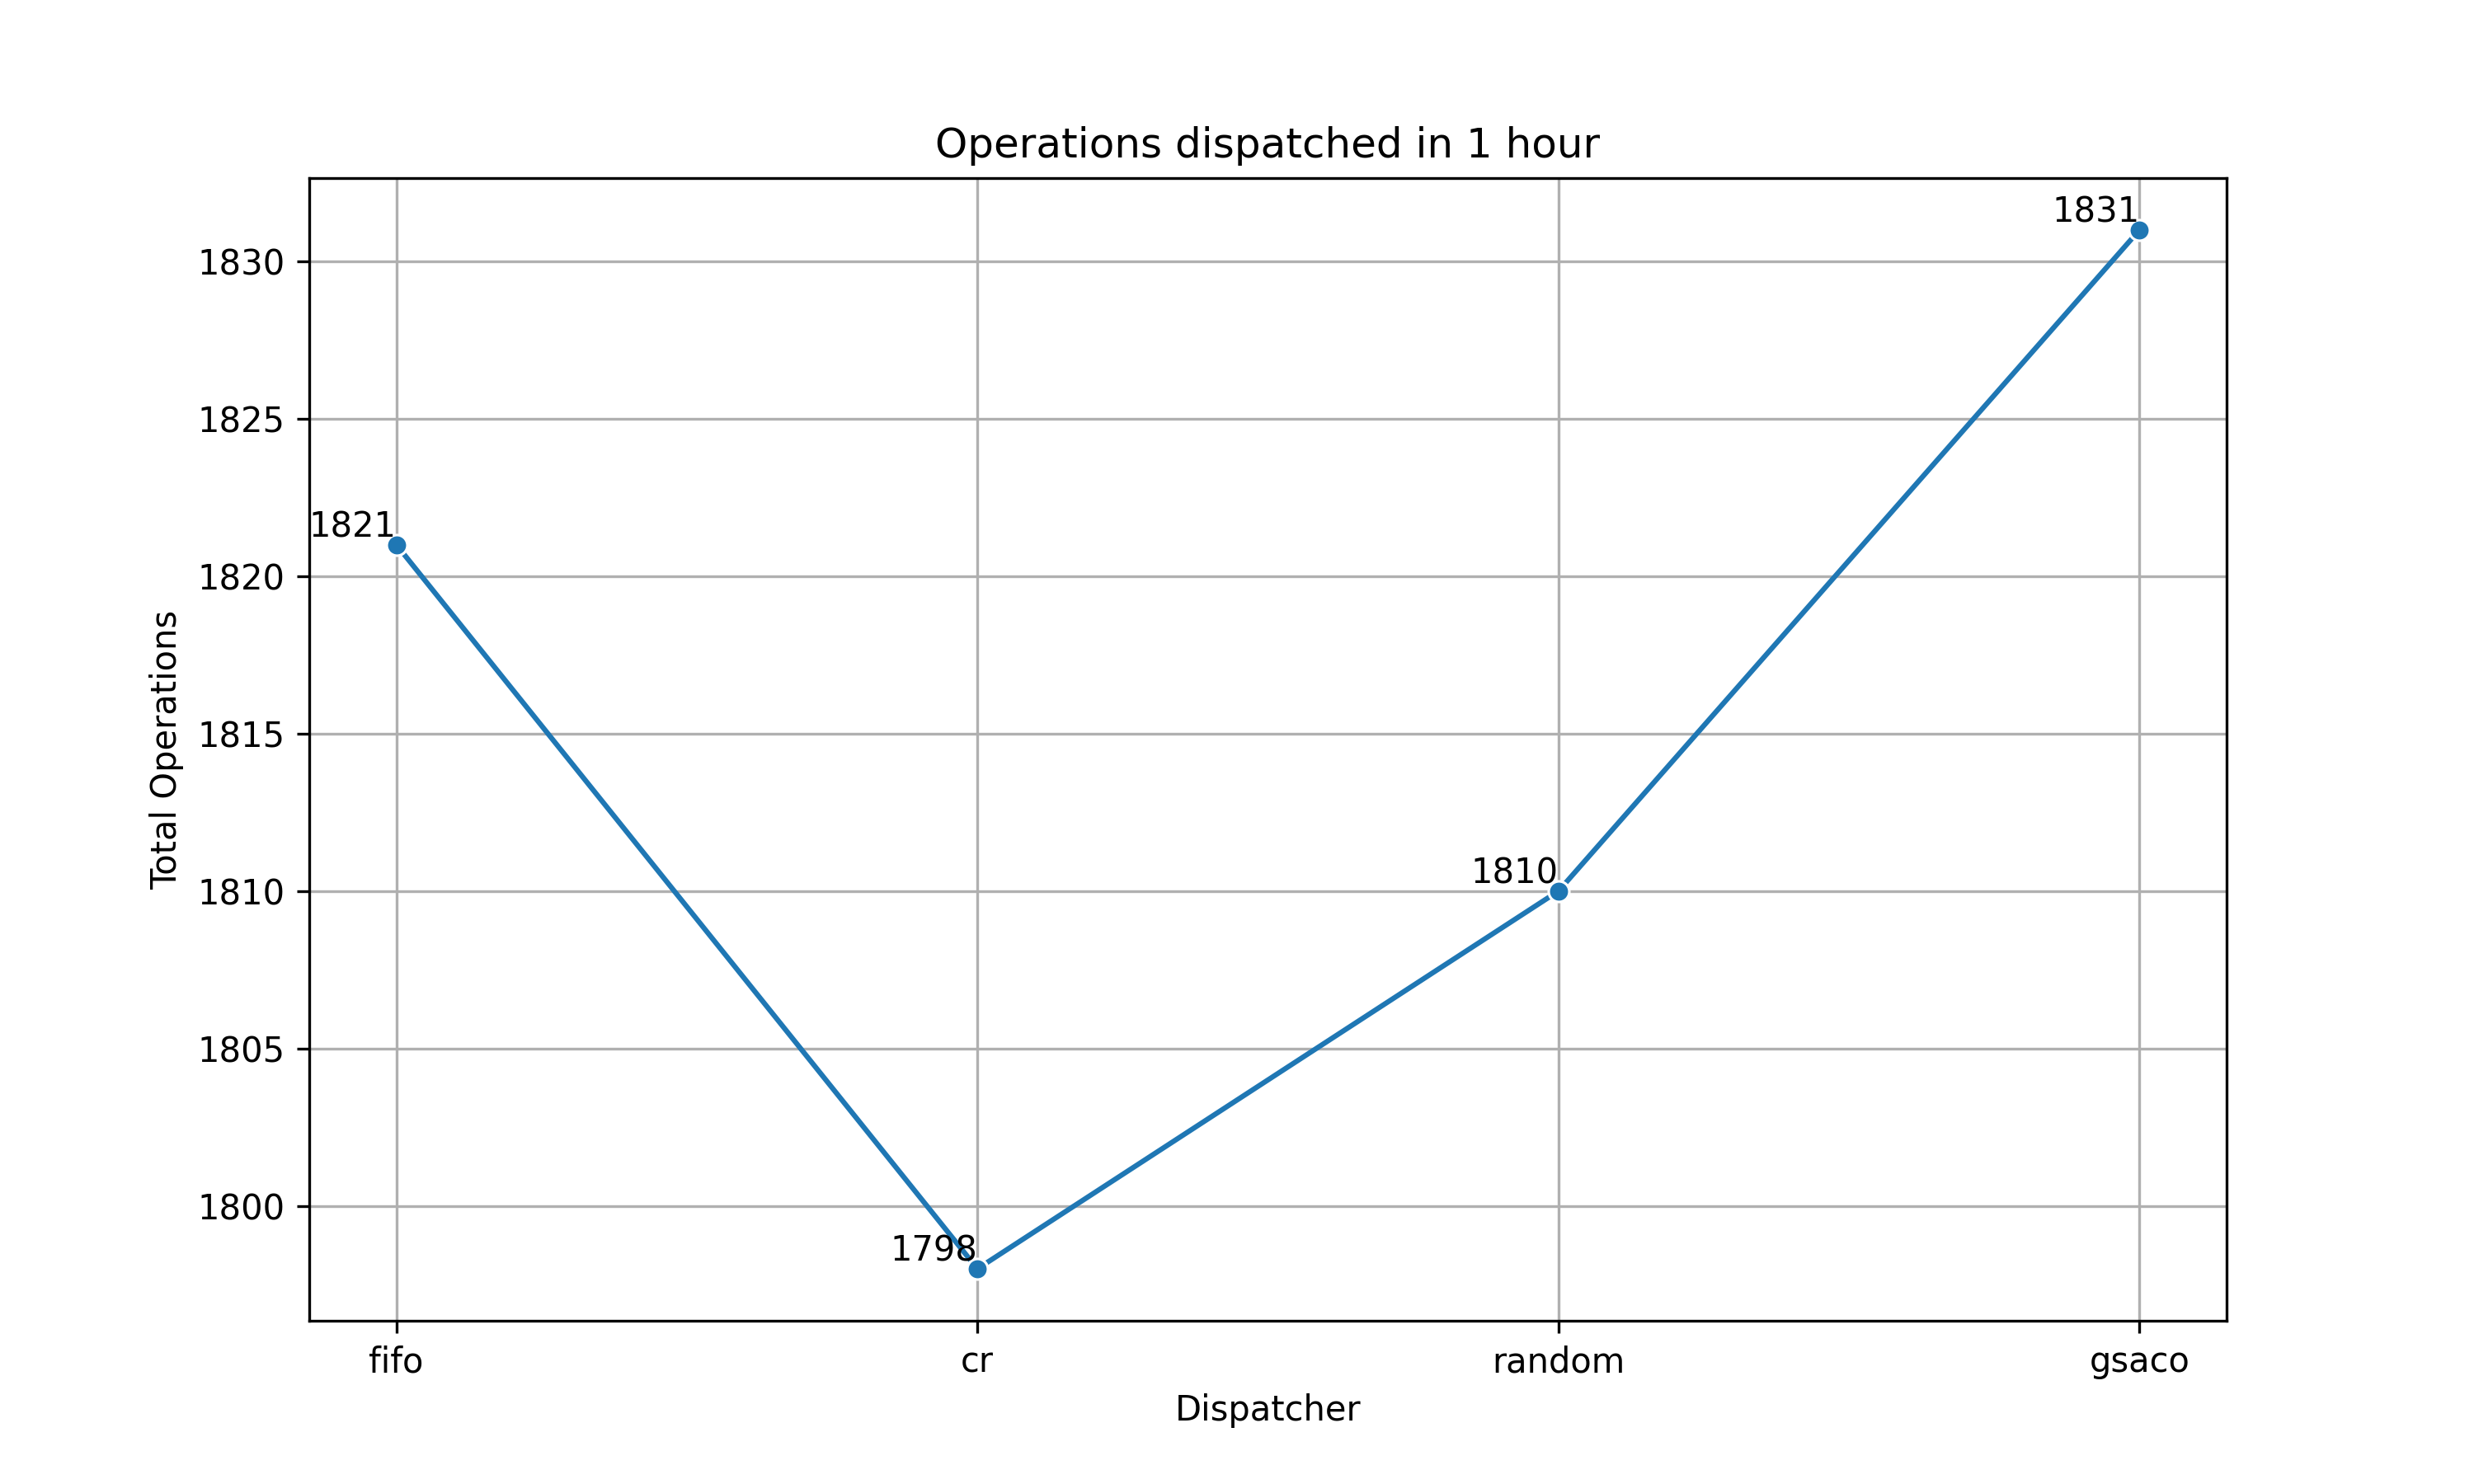
\includegraphics[width=\textwidth]{HVLM/total_operations_3600s.png}
		% \caption{}
		% \label{fig:o1}
	\end{subfigure}\hfill
	\begin{subfigure}{0.32\textwidth}
		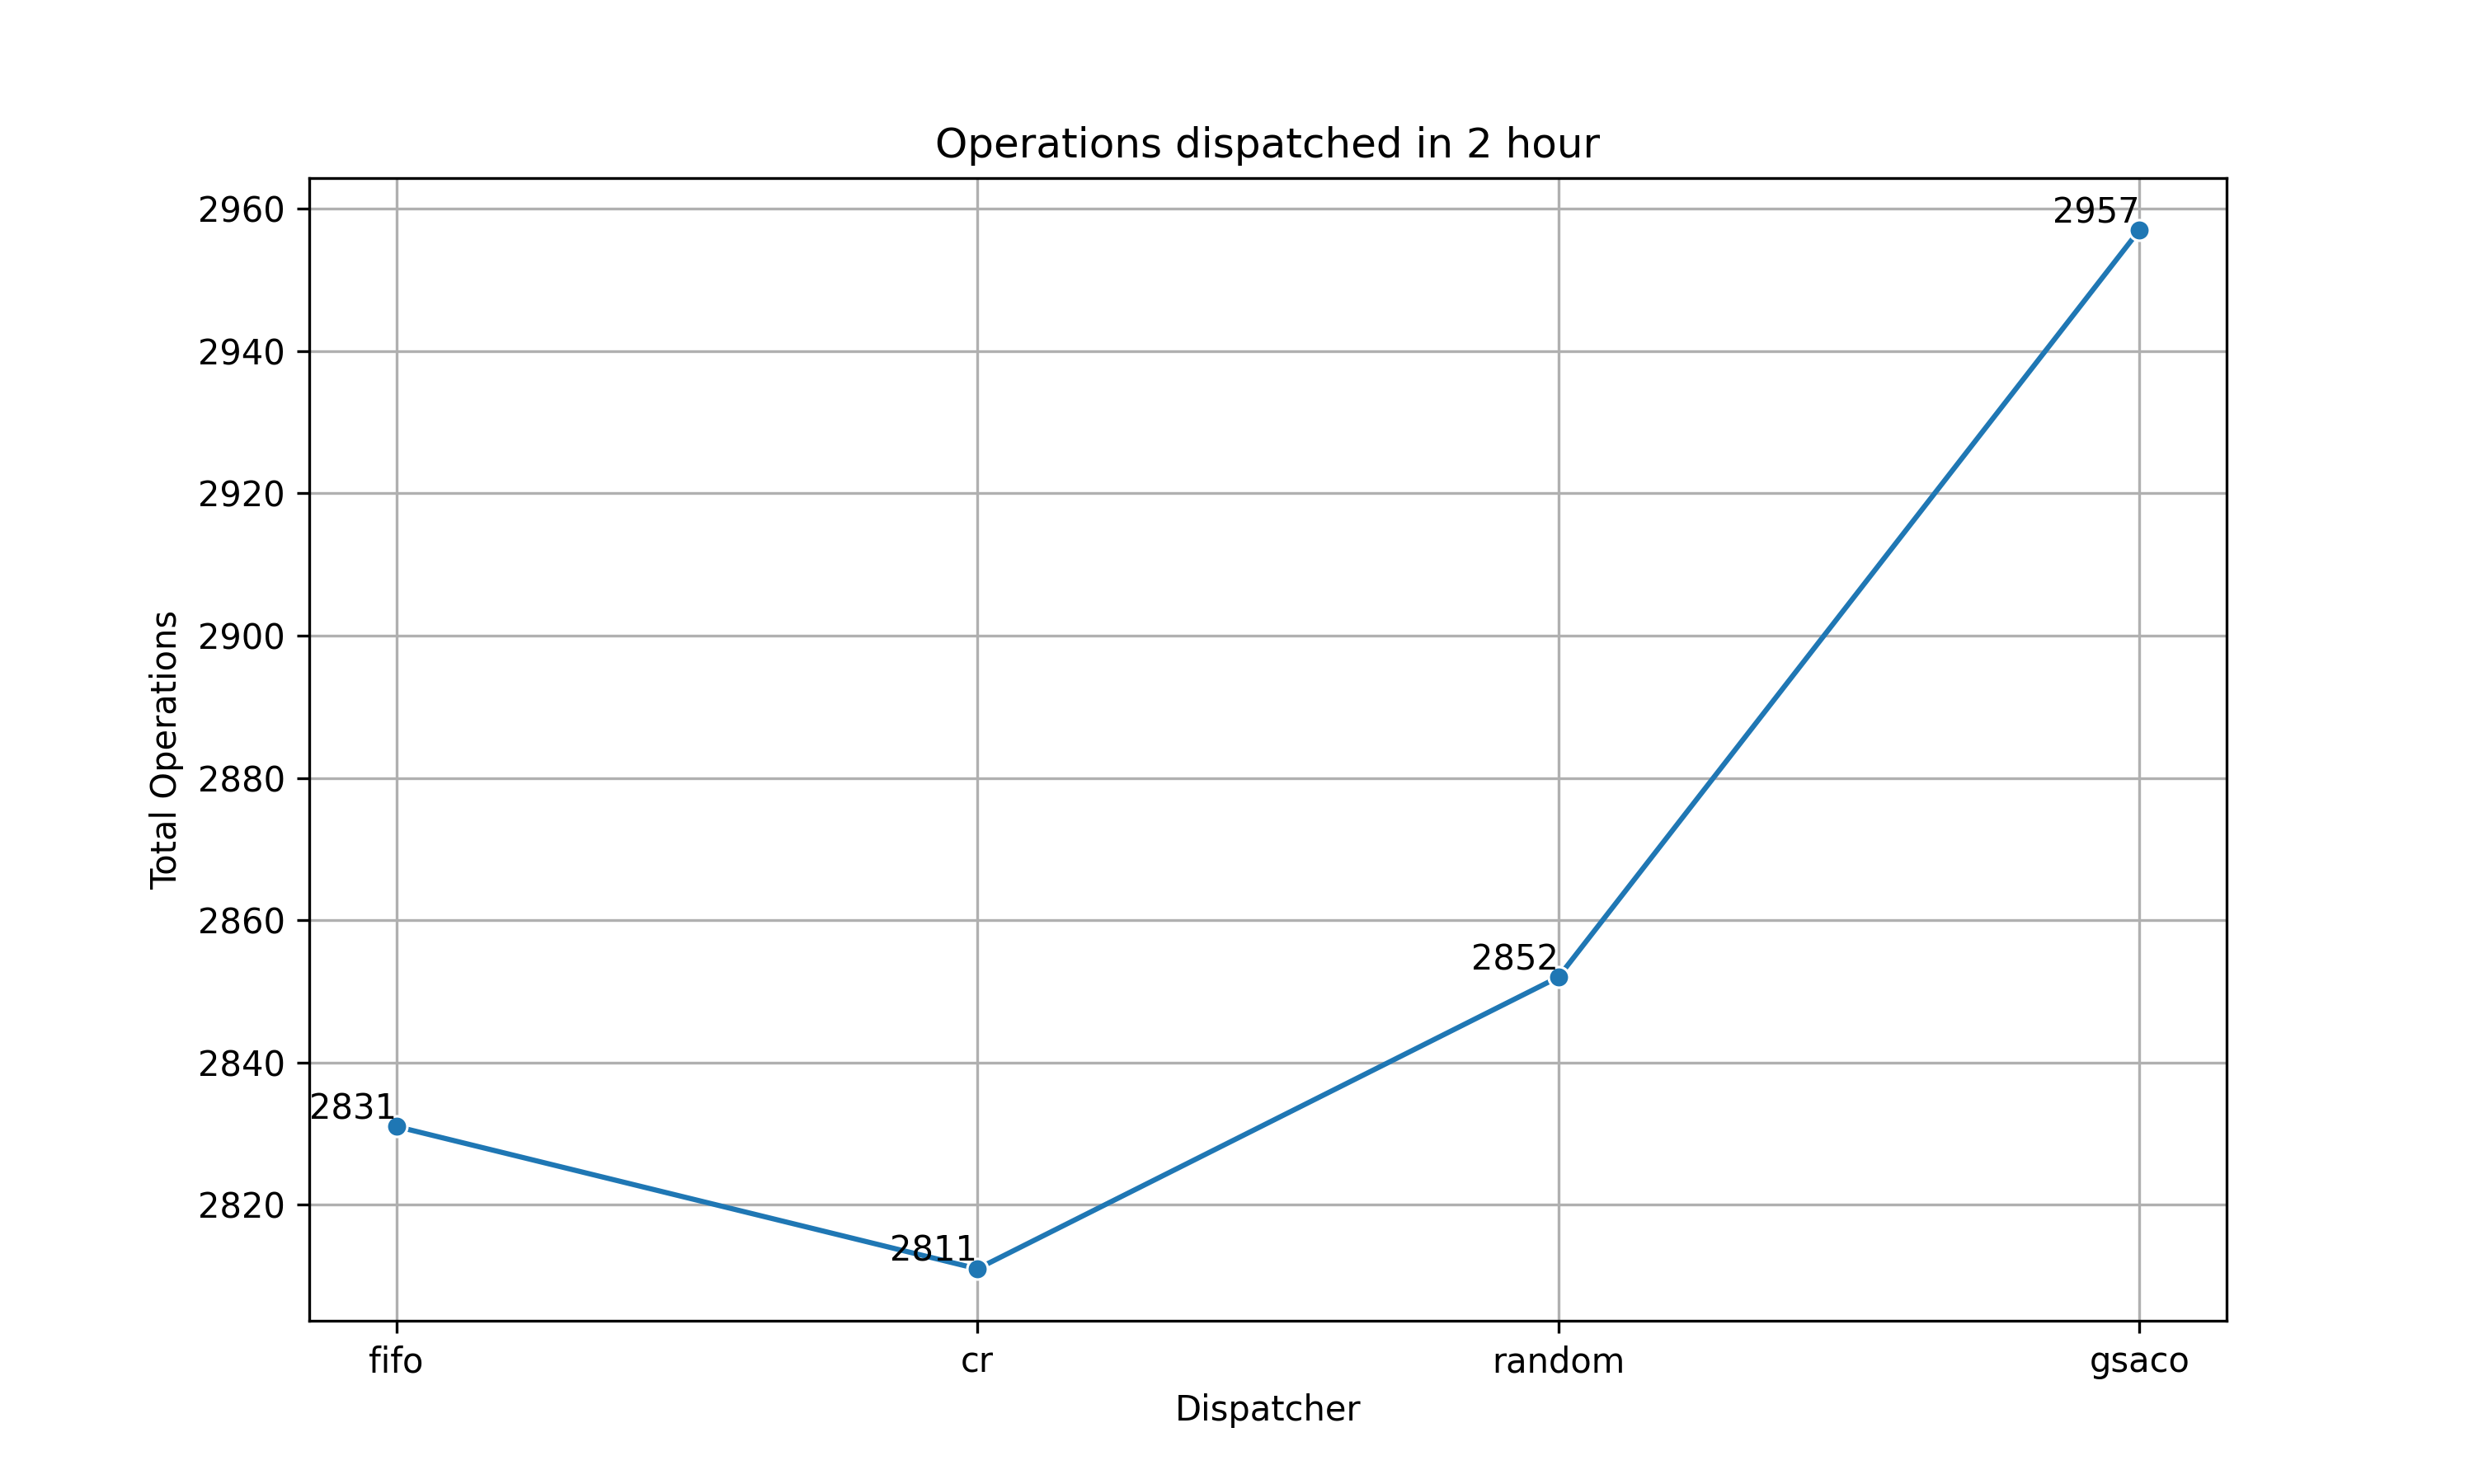
\includegraphics[width=\textwidth]{HVLM/total_operations_7200s.png}
		% \caption{}
		% \label{fig:o2}
	\end{subfigure}\hfill
	\begin{subfigure}{0.32\textwidth}
		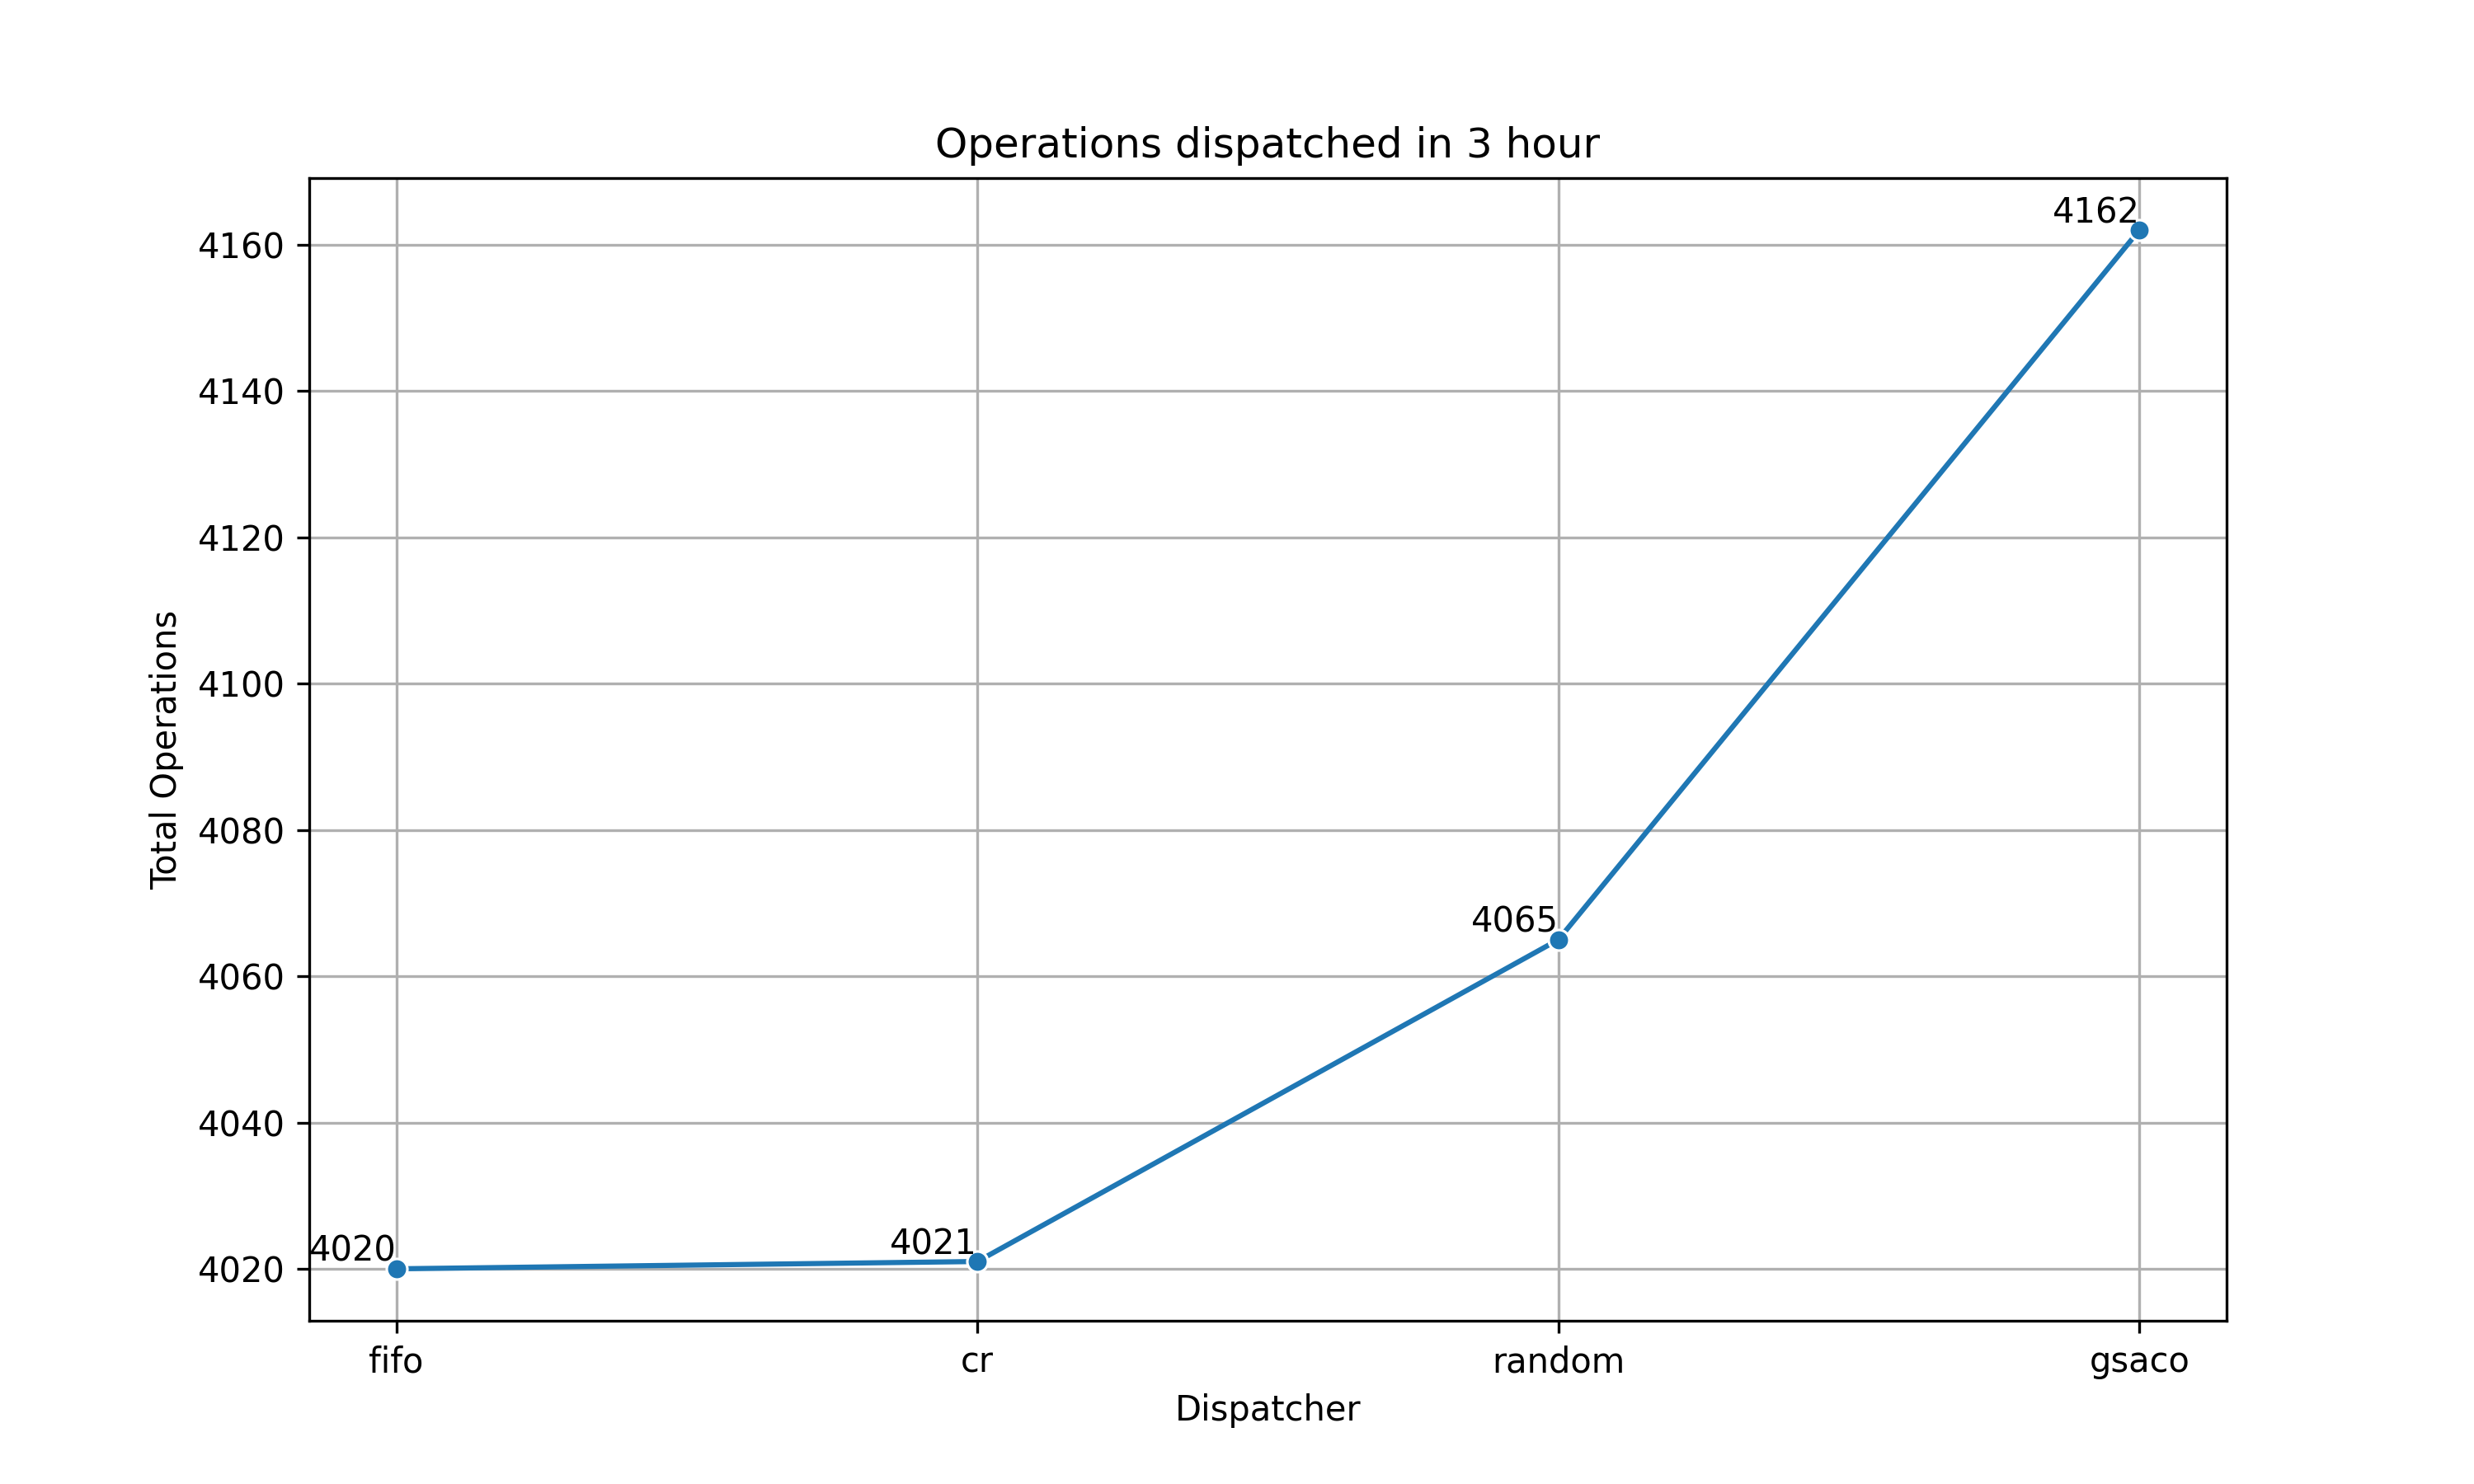
\includegraphics[width=\textwidth]{HVLM/total_operations_10800s.png}
		% \caption{}
		% \label{fig:o3}
	\end{subfigure}
	\begin{subfigure}{0.32\textwidth}
		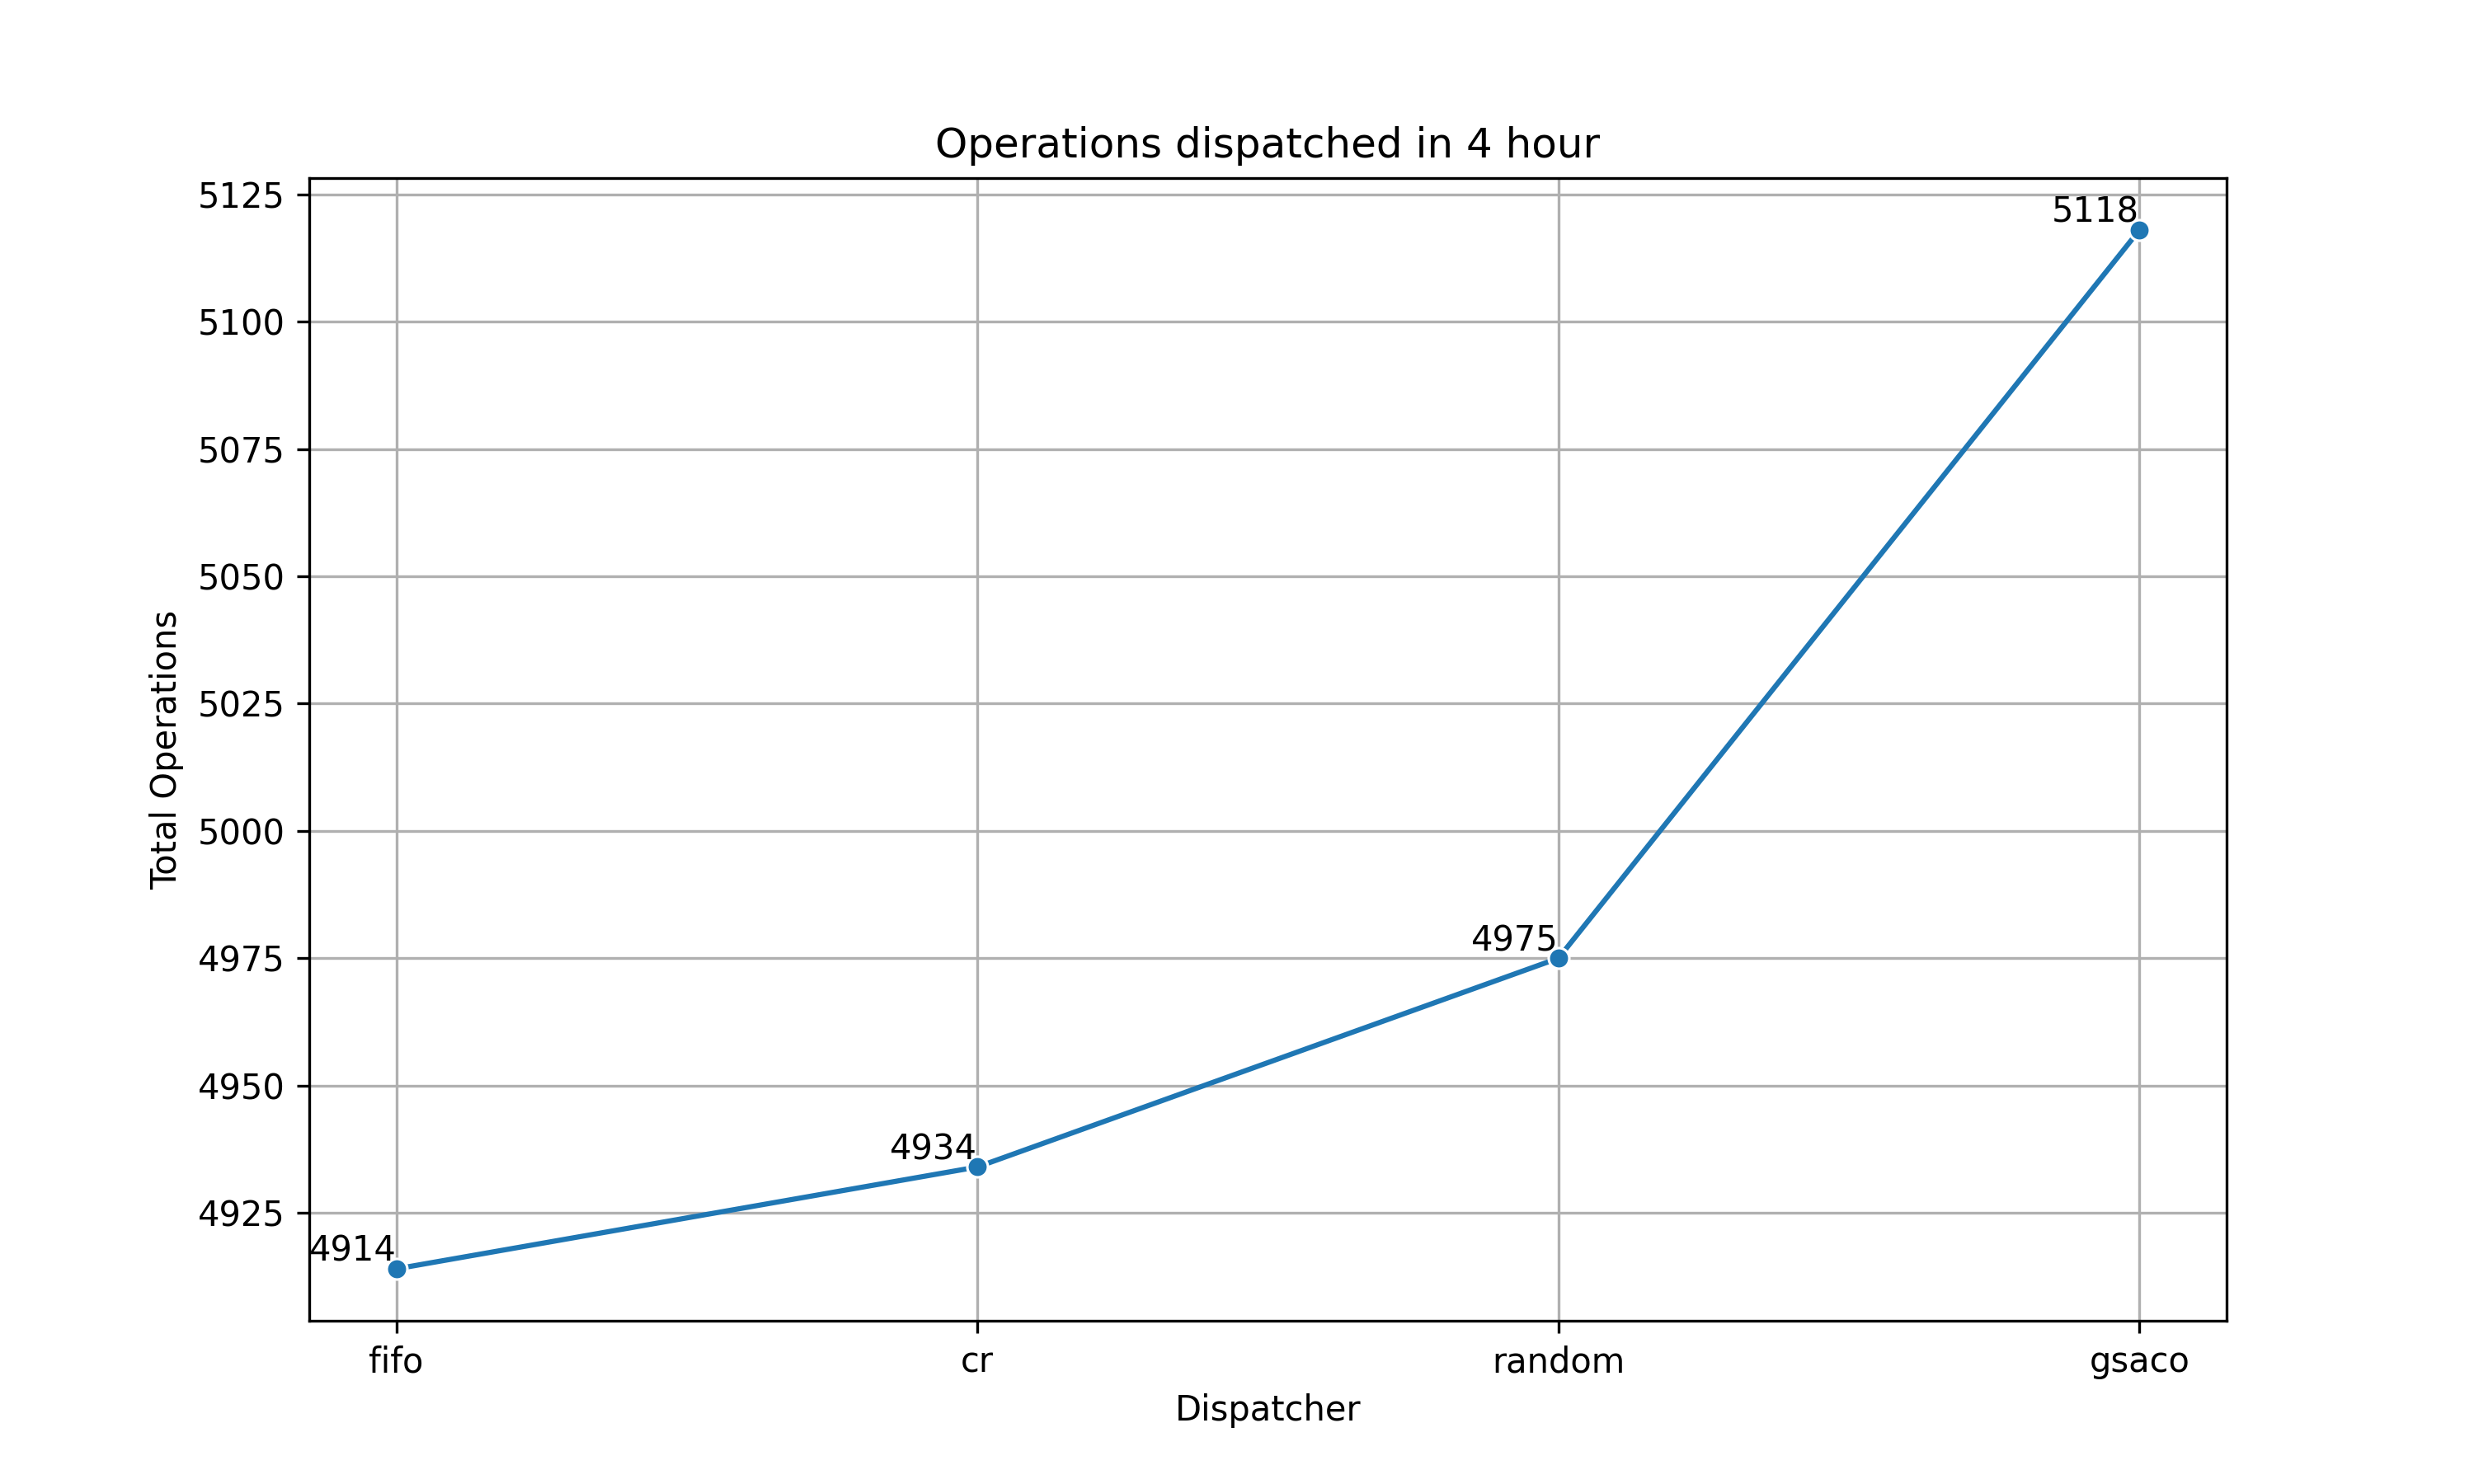
\includegraphics[width=\textwidth]{HVLM/total_operations_14400s.png}
		% \caption{}
		% \label{fig:o4}
	\end{subfigure}\hfill
	\begin{subfigure}{0.32\textwidth}
		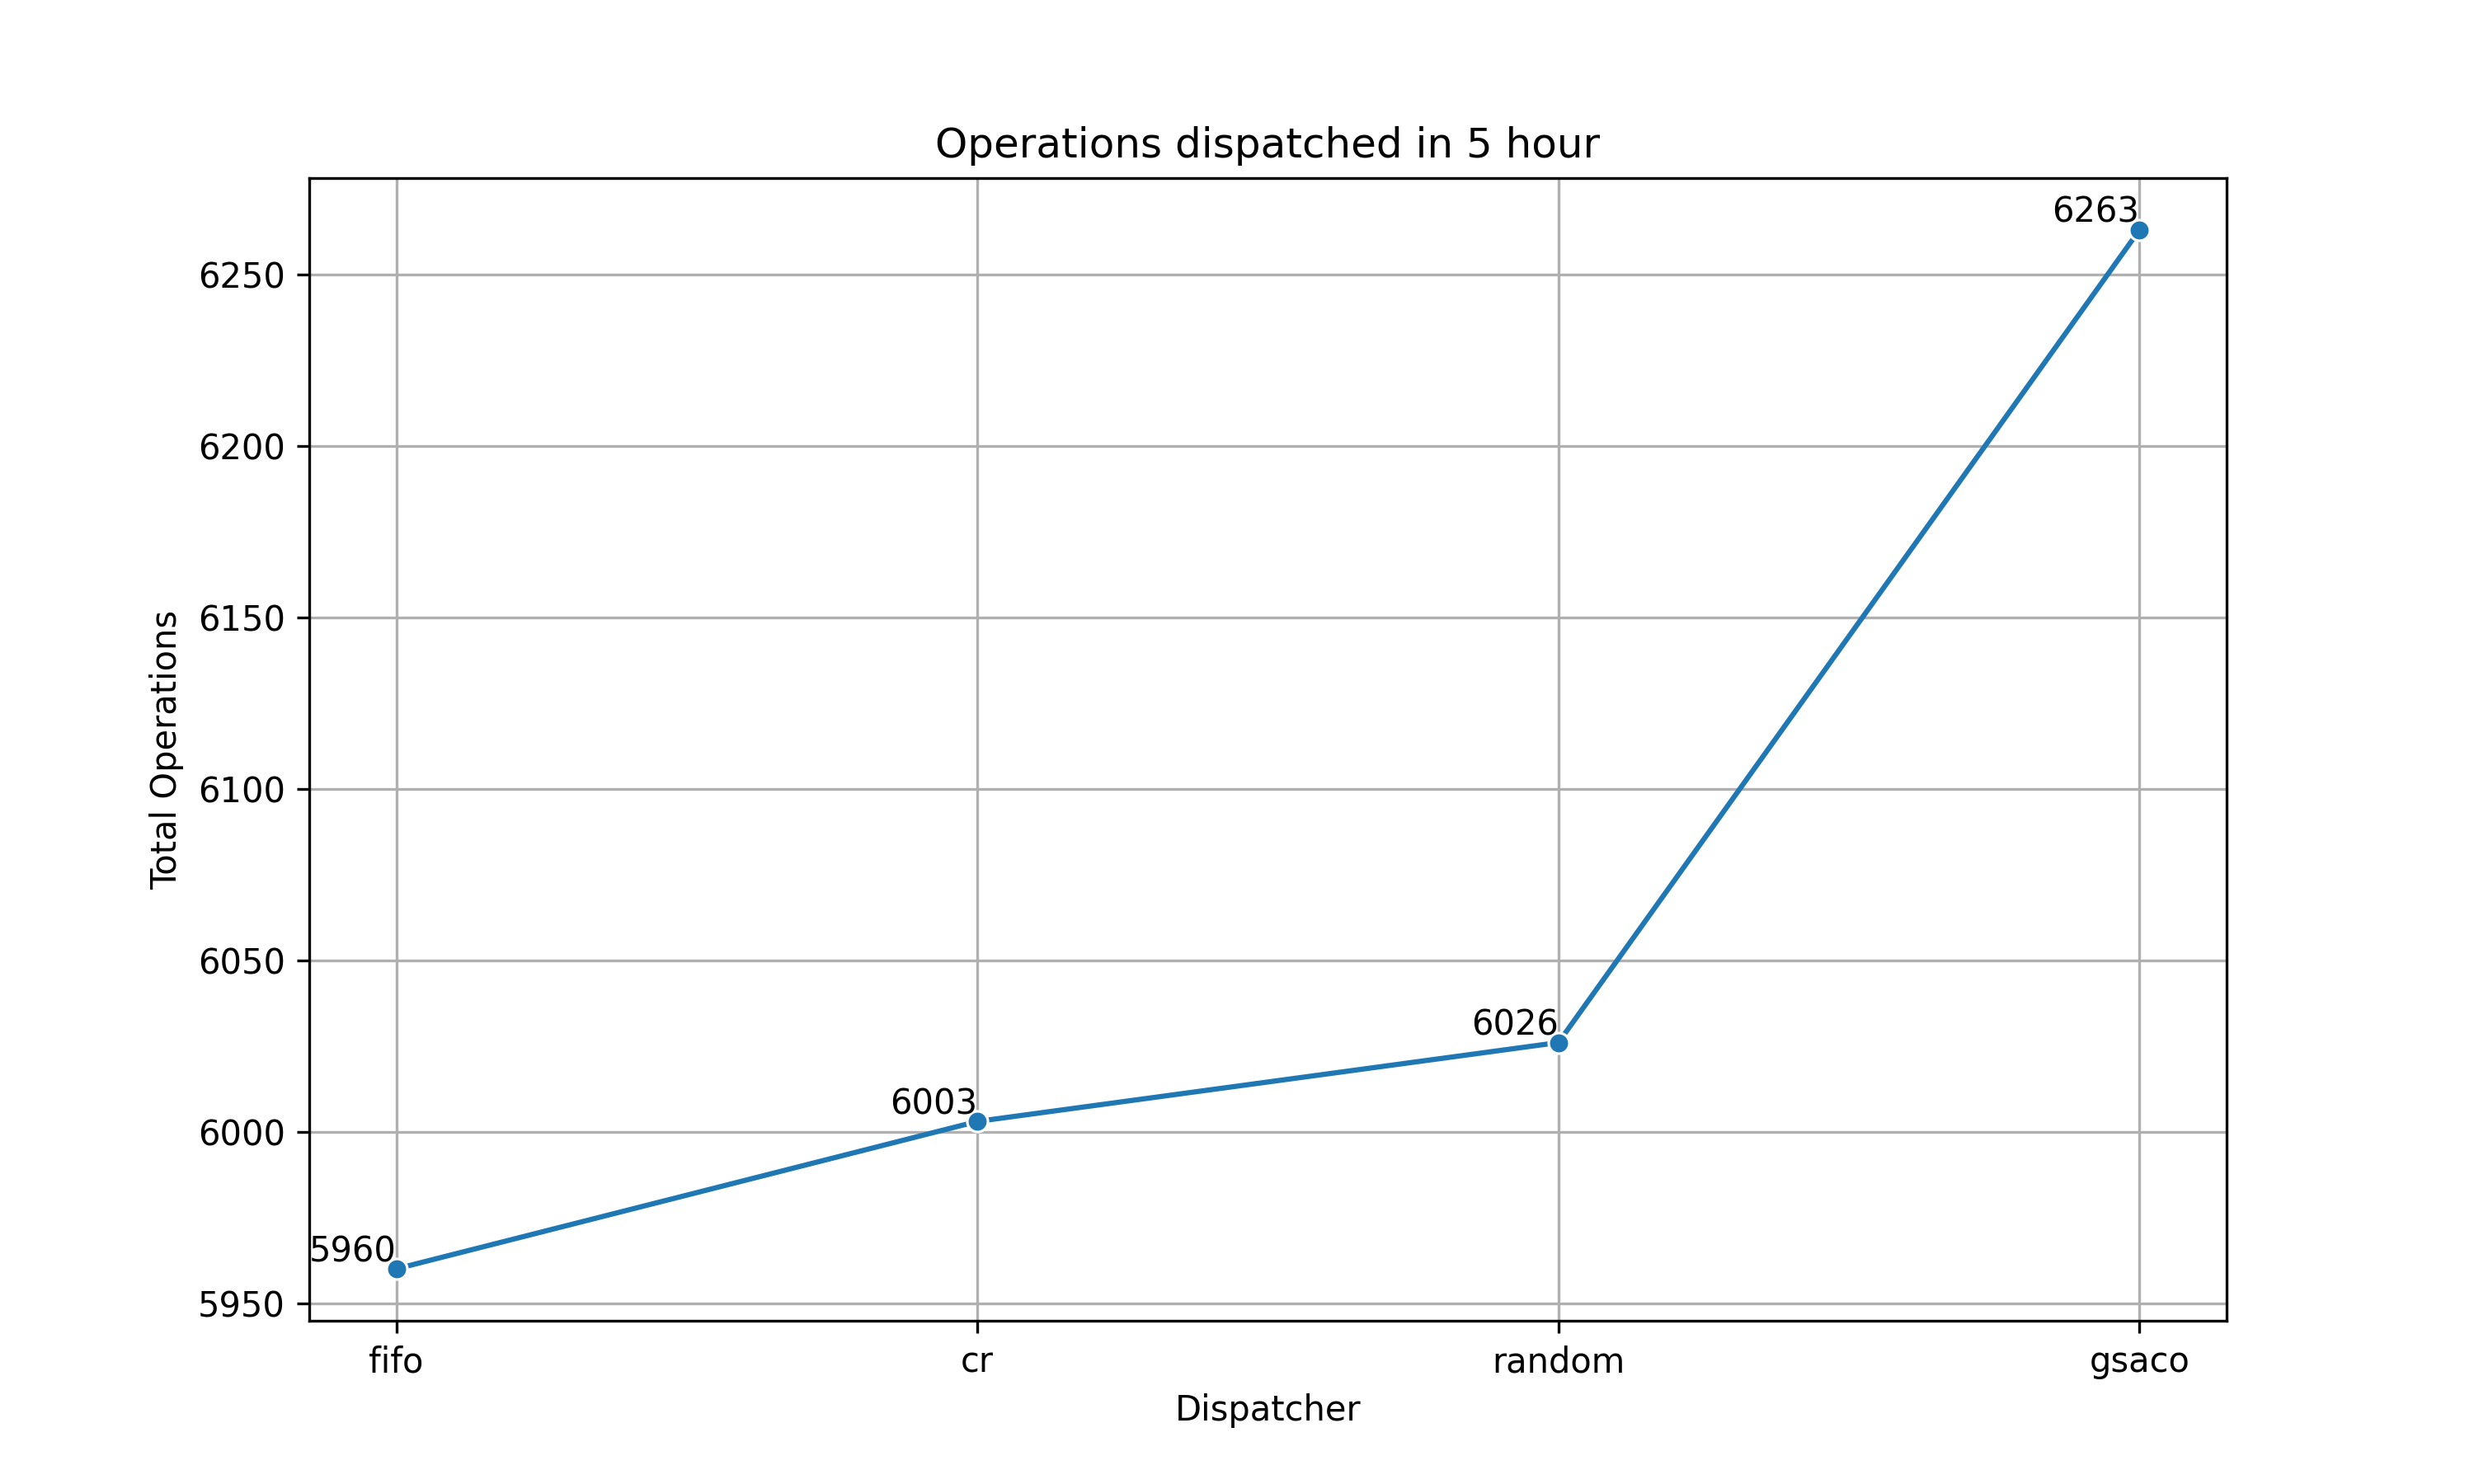
\includegraphics[width=\textwidth]{HVLM/total_operations_18000s.png}
		% \caption{}
		% \label{fig:o5}
	\end{subfigure}\hfill
	\begin{subfigure}{0.32\textwidth}
		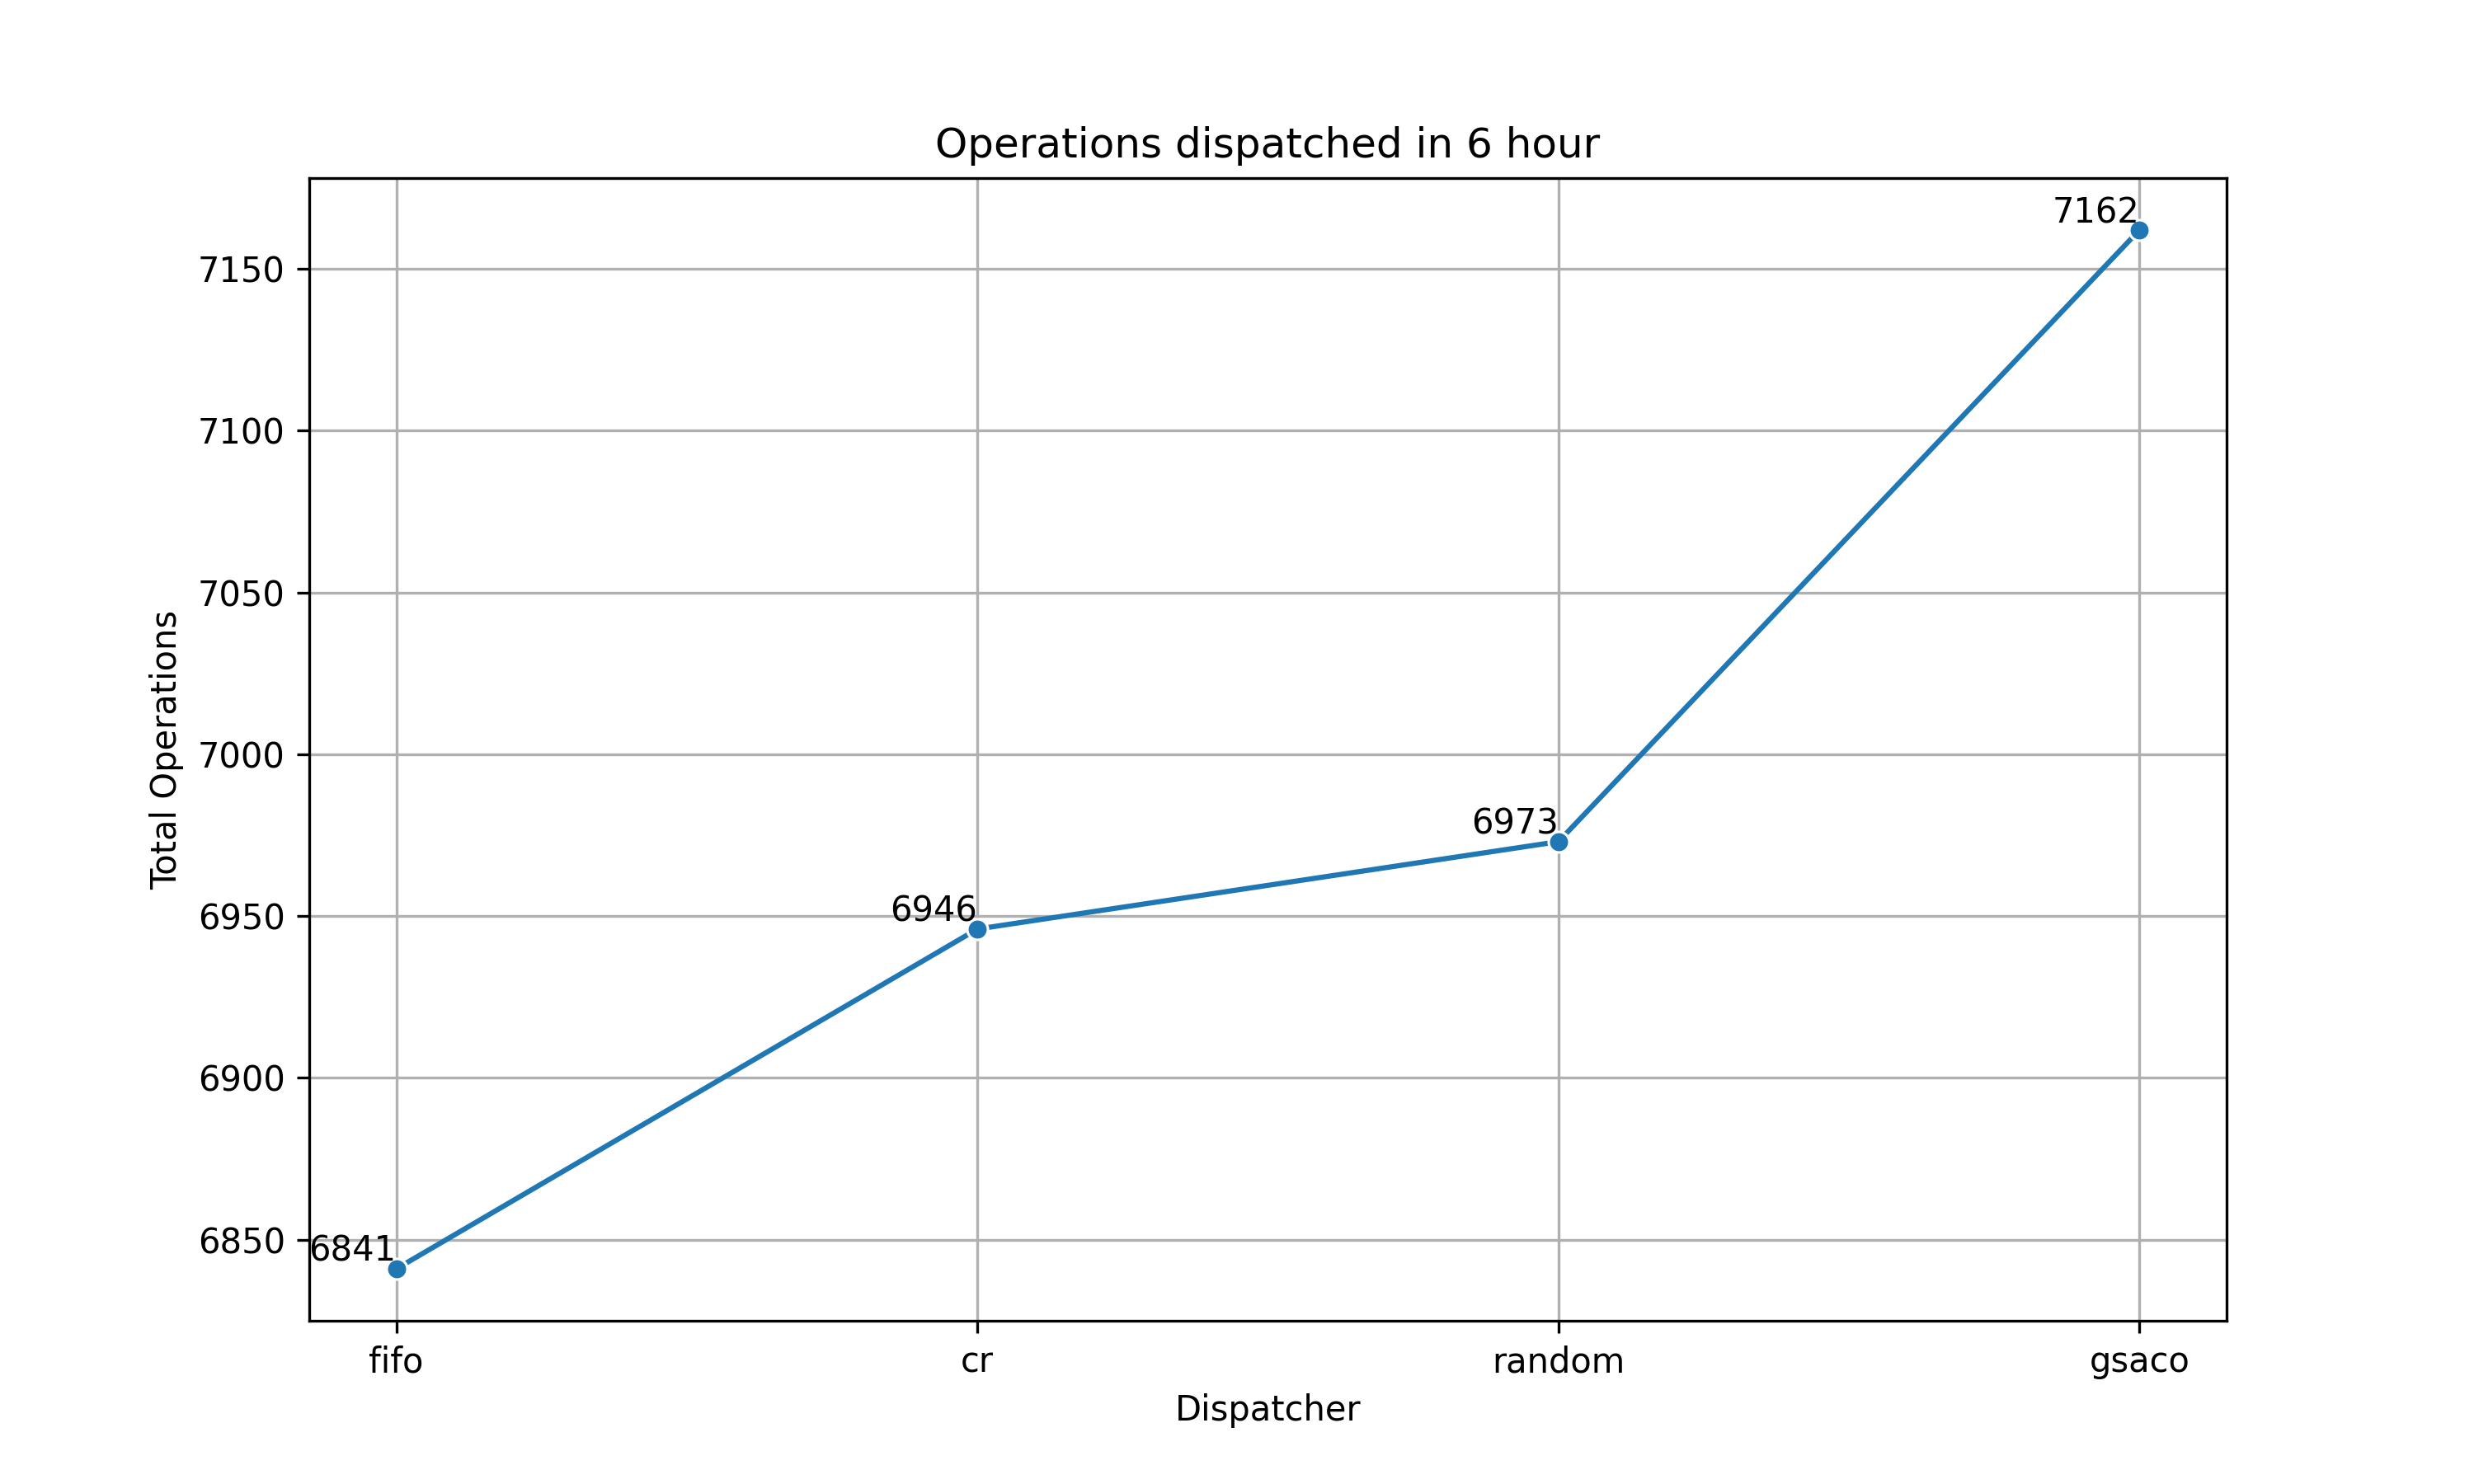
\includegraphics[width=\textwidth]{HVLM/total_operations_21600s.png}
		% \caption{}
		% \label{fig:o6}
	\end{subfigure}
	\caption{Completed operations for HV/LM}
	\label{fig:totalopsHVLM}
\end{figure}

\begin{figure}[t]
	\centering
	\begin{subfigure}[b]{0.32\textwidth}
		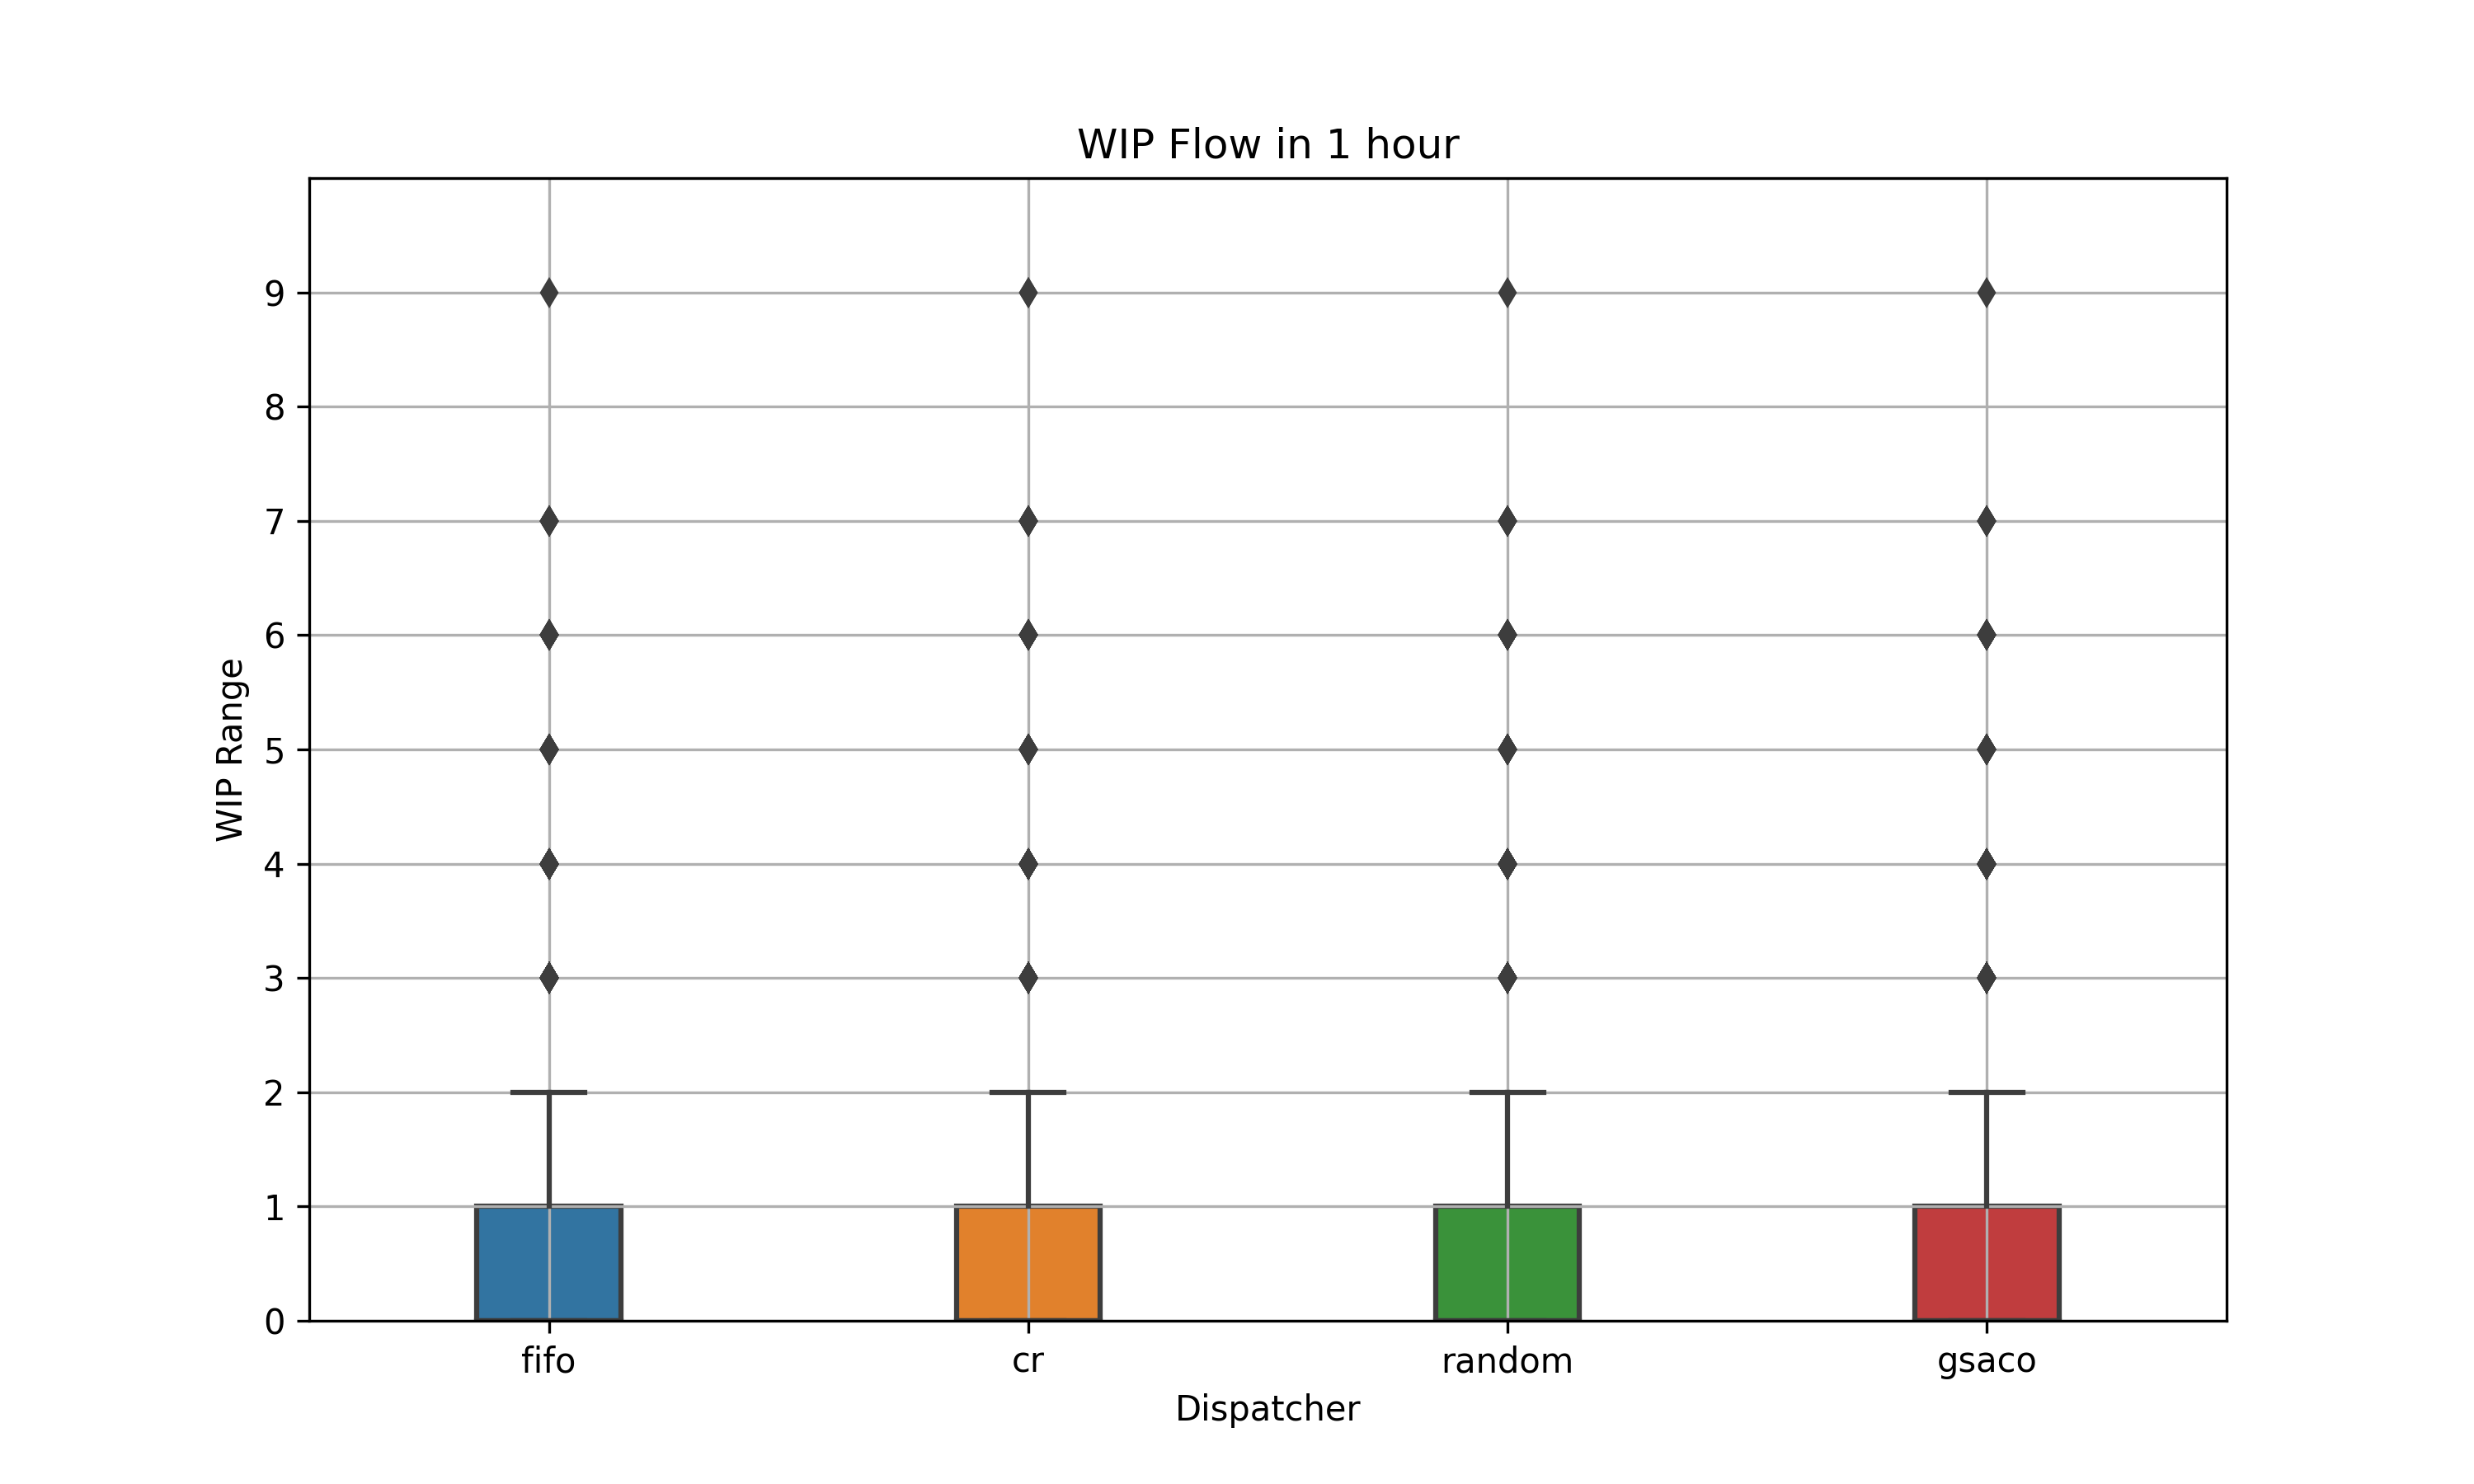
\includegraphics[width=\textwidth]{HVLM/period_3600s.png}
		% \caption{}
		% \label{fig:p1}
	\end{subfigure}
	\hfill
	\begin{subfigure}[b]{0.32\textwidth}
		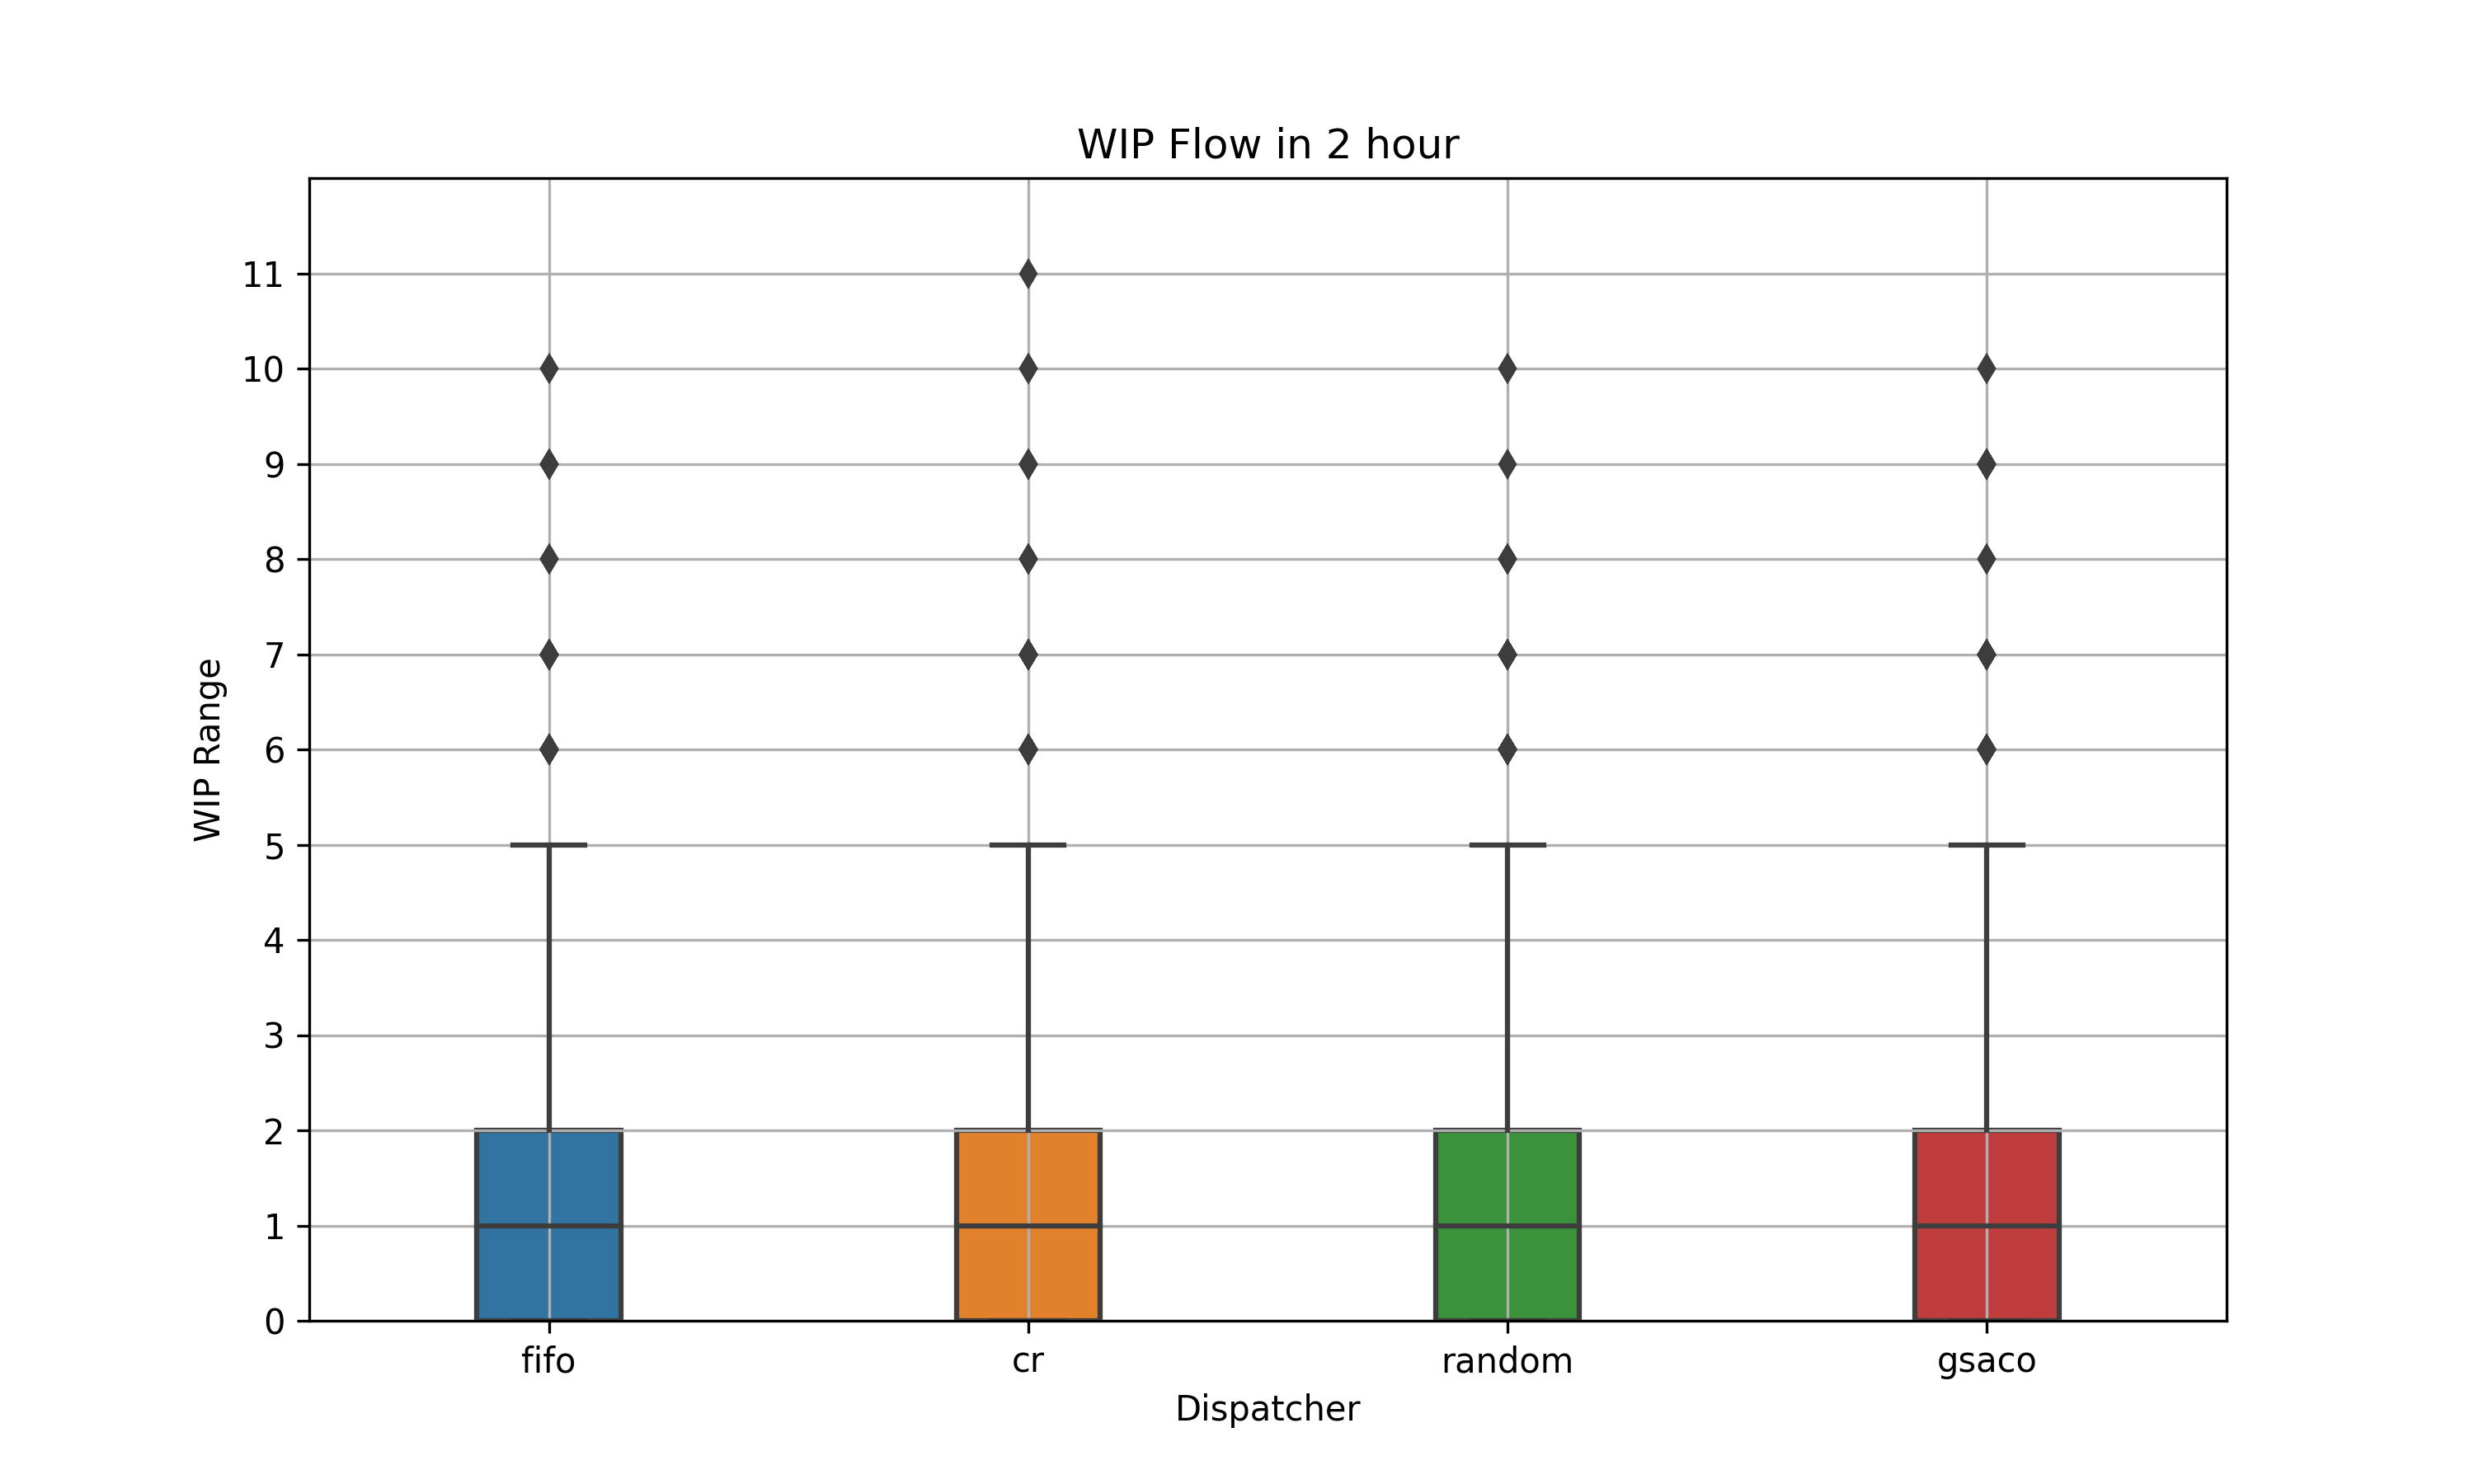
\includegraphics[width=\textwidth]{HVLM/period_7200s.png}
		% \caption{}
		% \label{fig:p2}
	\end{subfigure}
	\hfill
	\begin{subfigure}[b]{0.32\textwidth}
		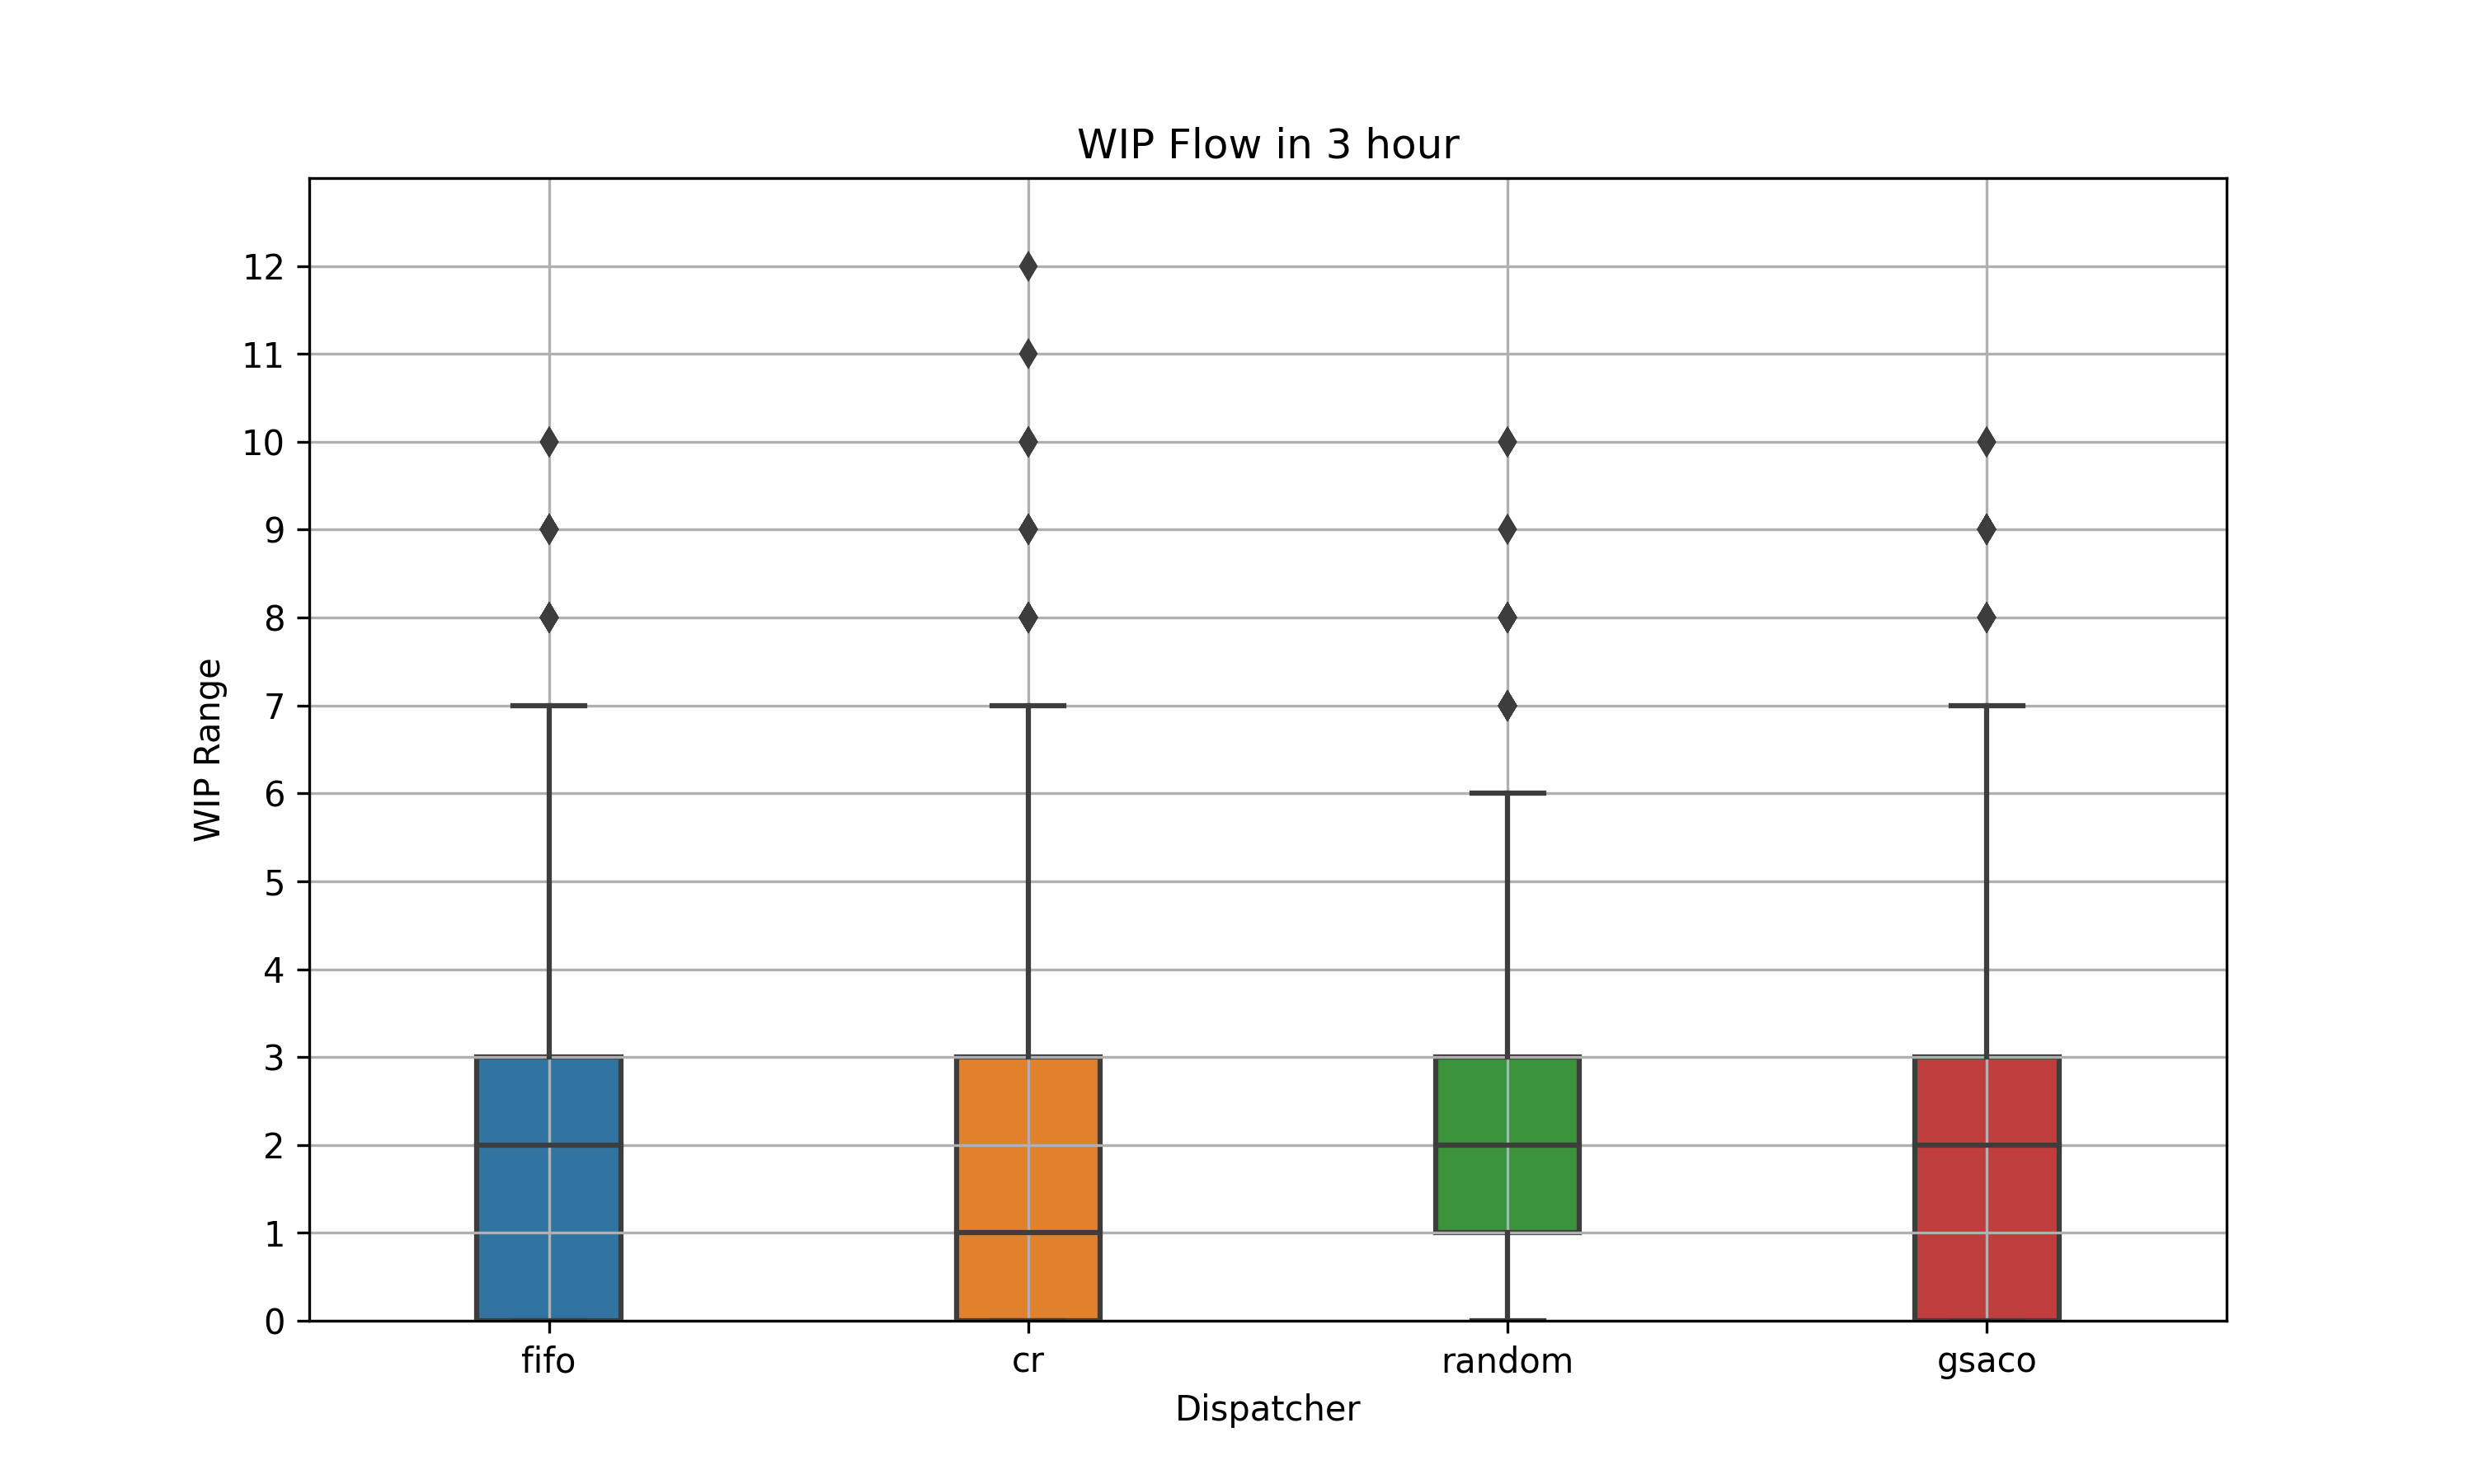
\includegraphics[width=\textwidth]{HVLM/period_10800s.png}
		% \caption{}
		% \label{fig:p3}
	\end{subfigure}
	
	\begin{subfigure}[b]{0.32\textwidth}
		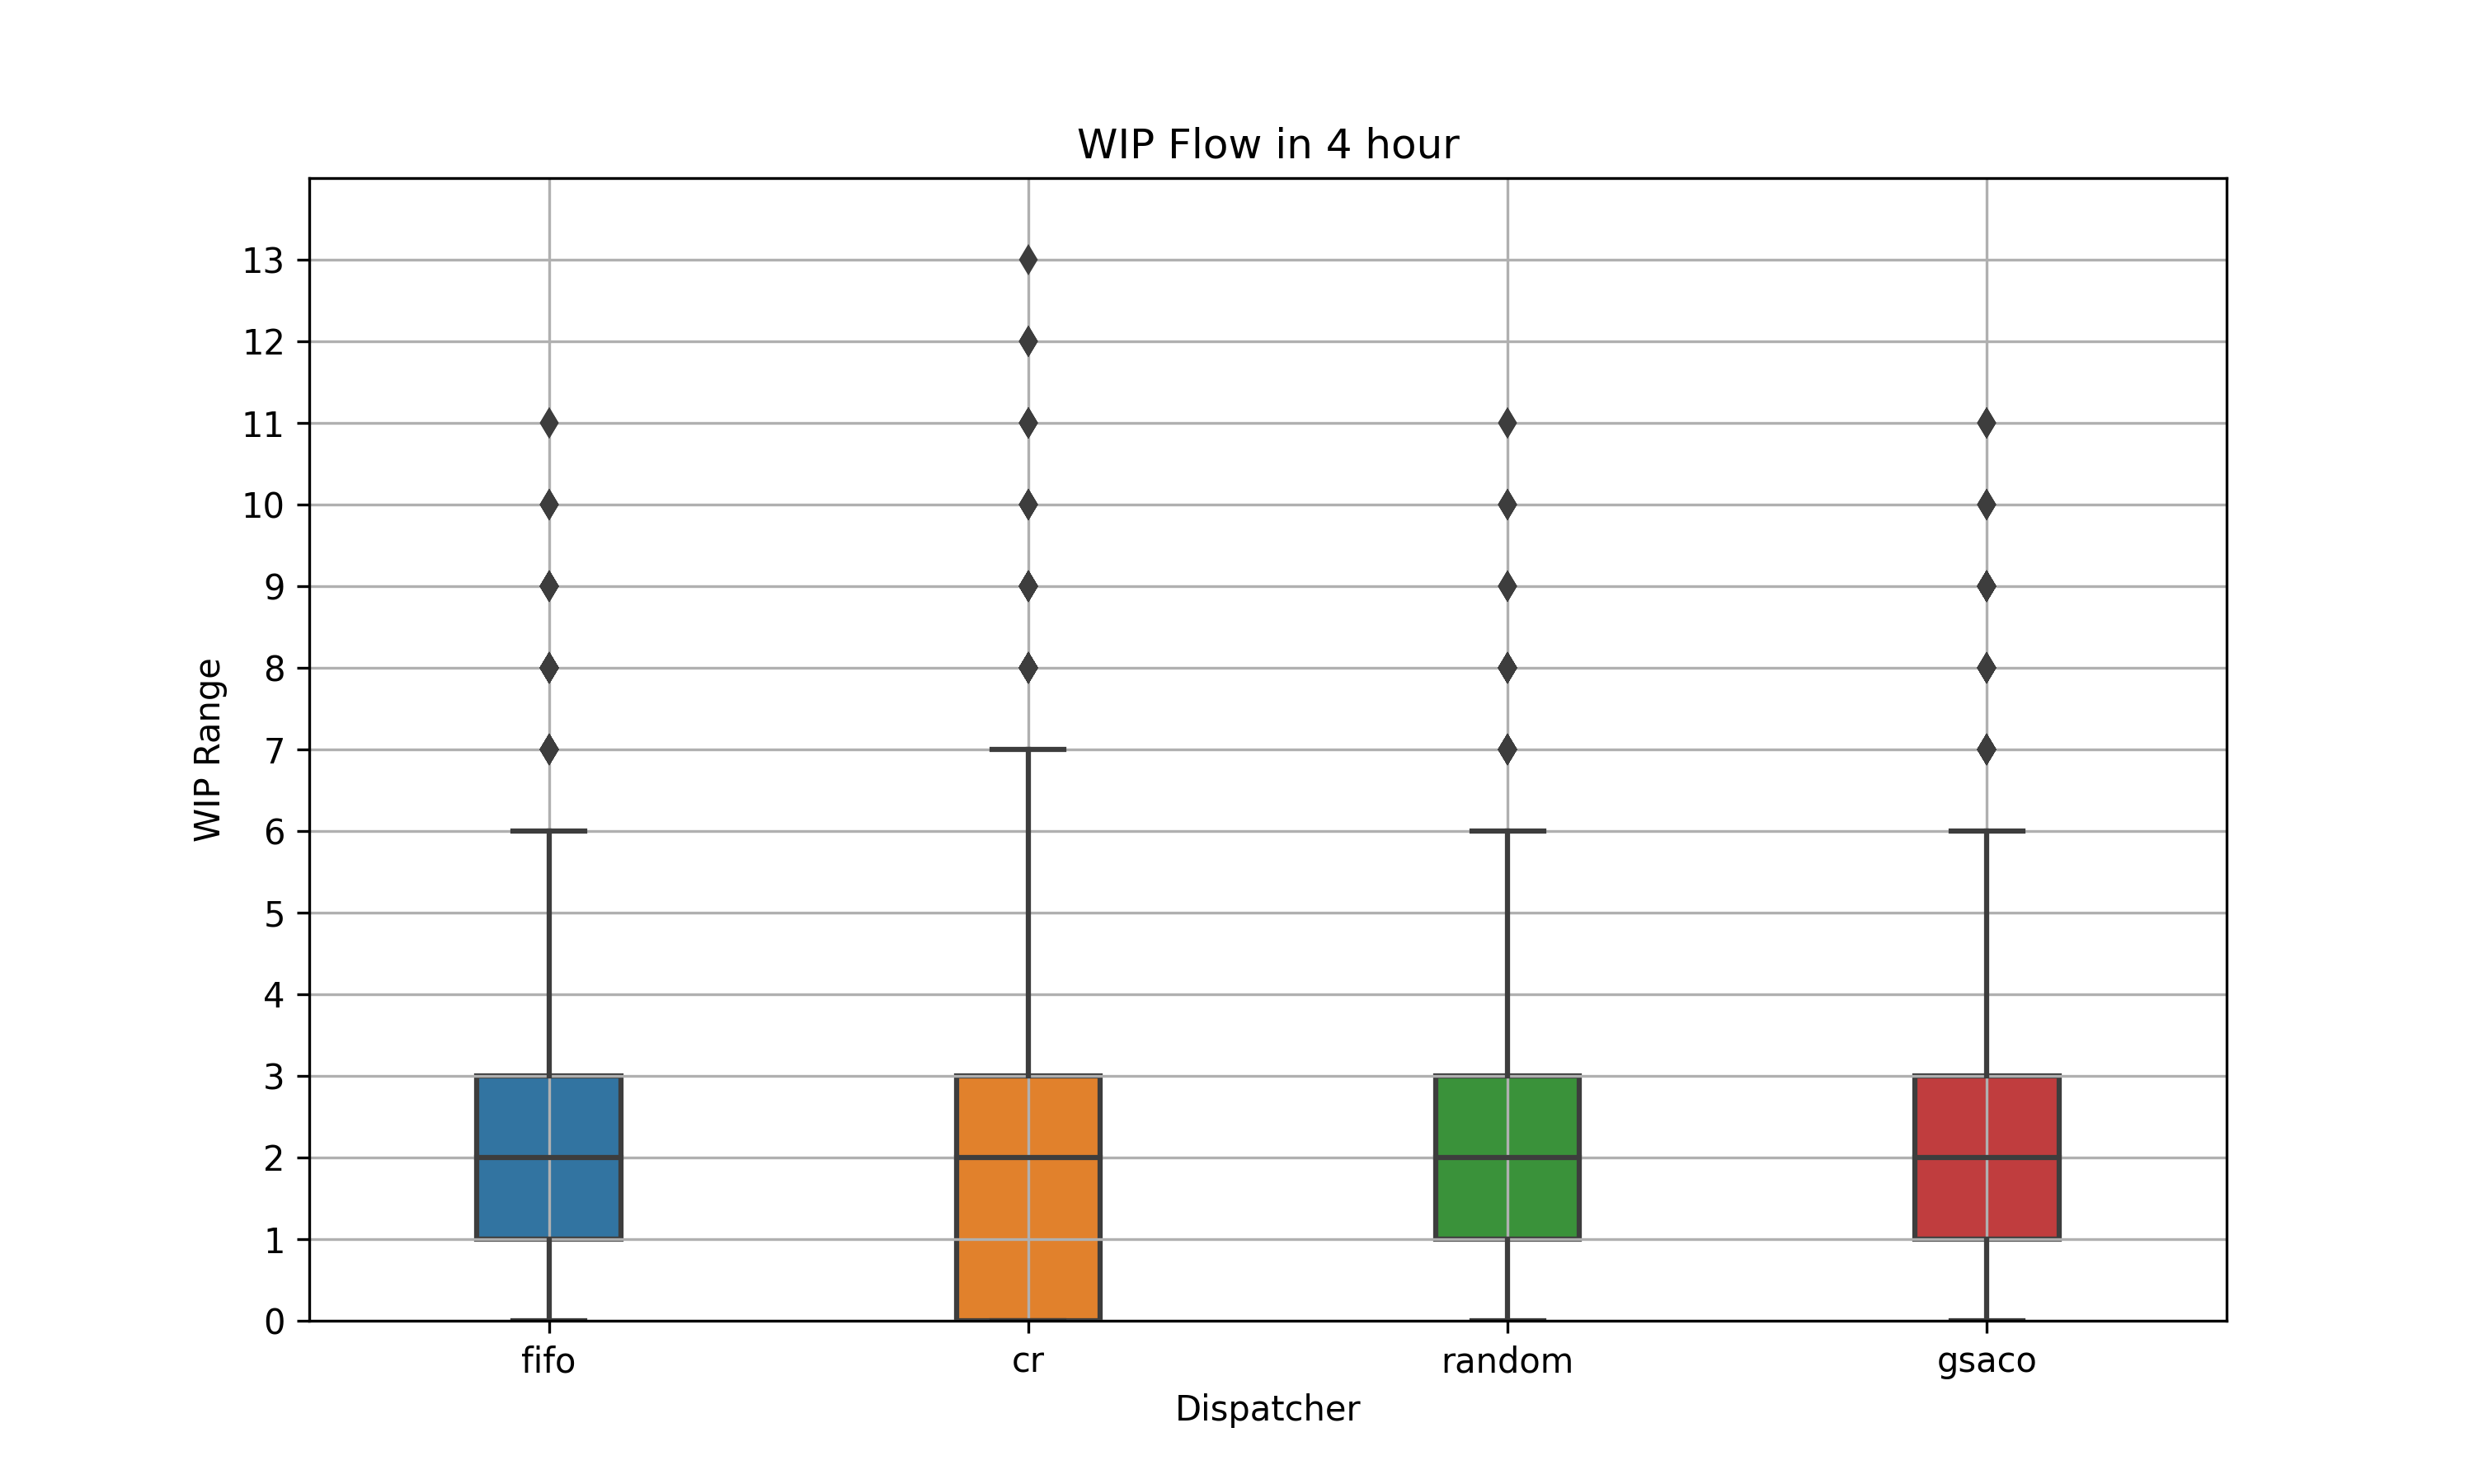
\includegraphics[width=\textwidth]{HVLM/period_14400s.png}
		% \caption{}
		% \label{fig:p4}
	\end{subfigure}
	\hfill
	\begin{subfigure}[b]{0.32\textwidth}
		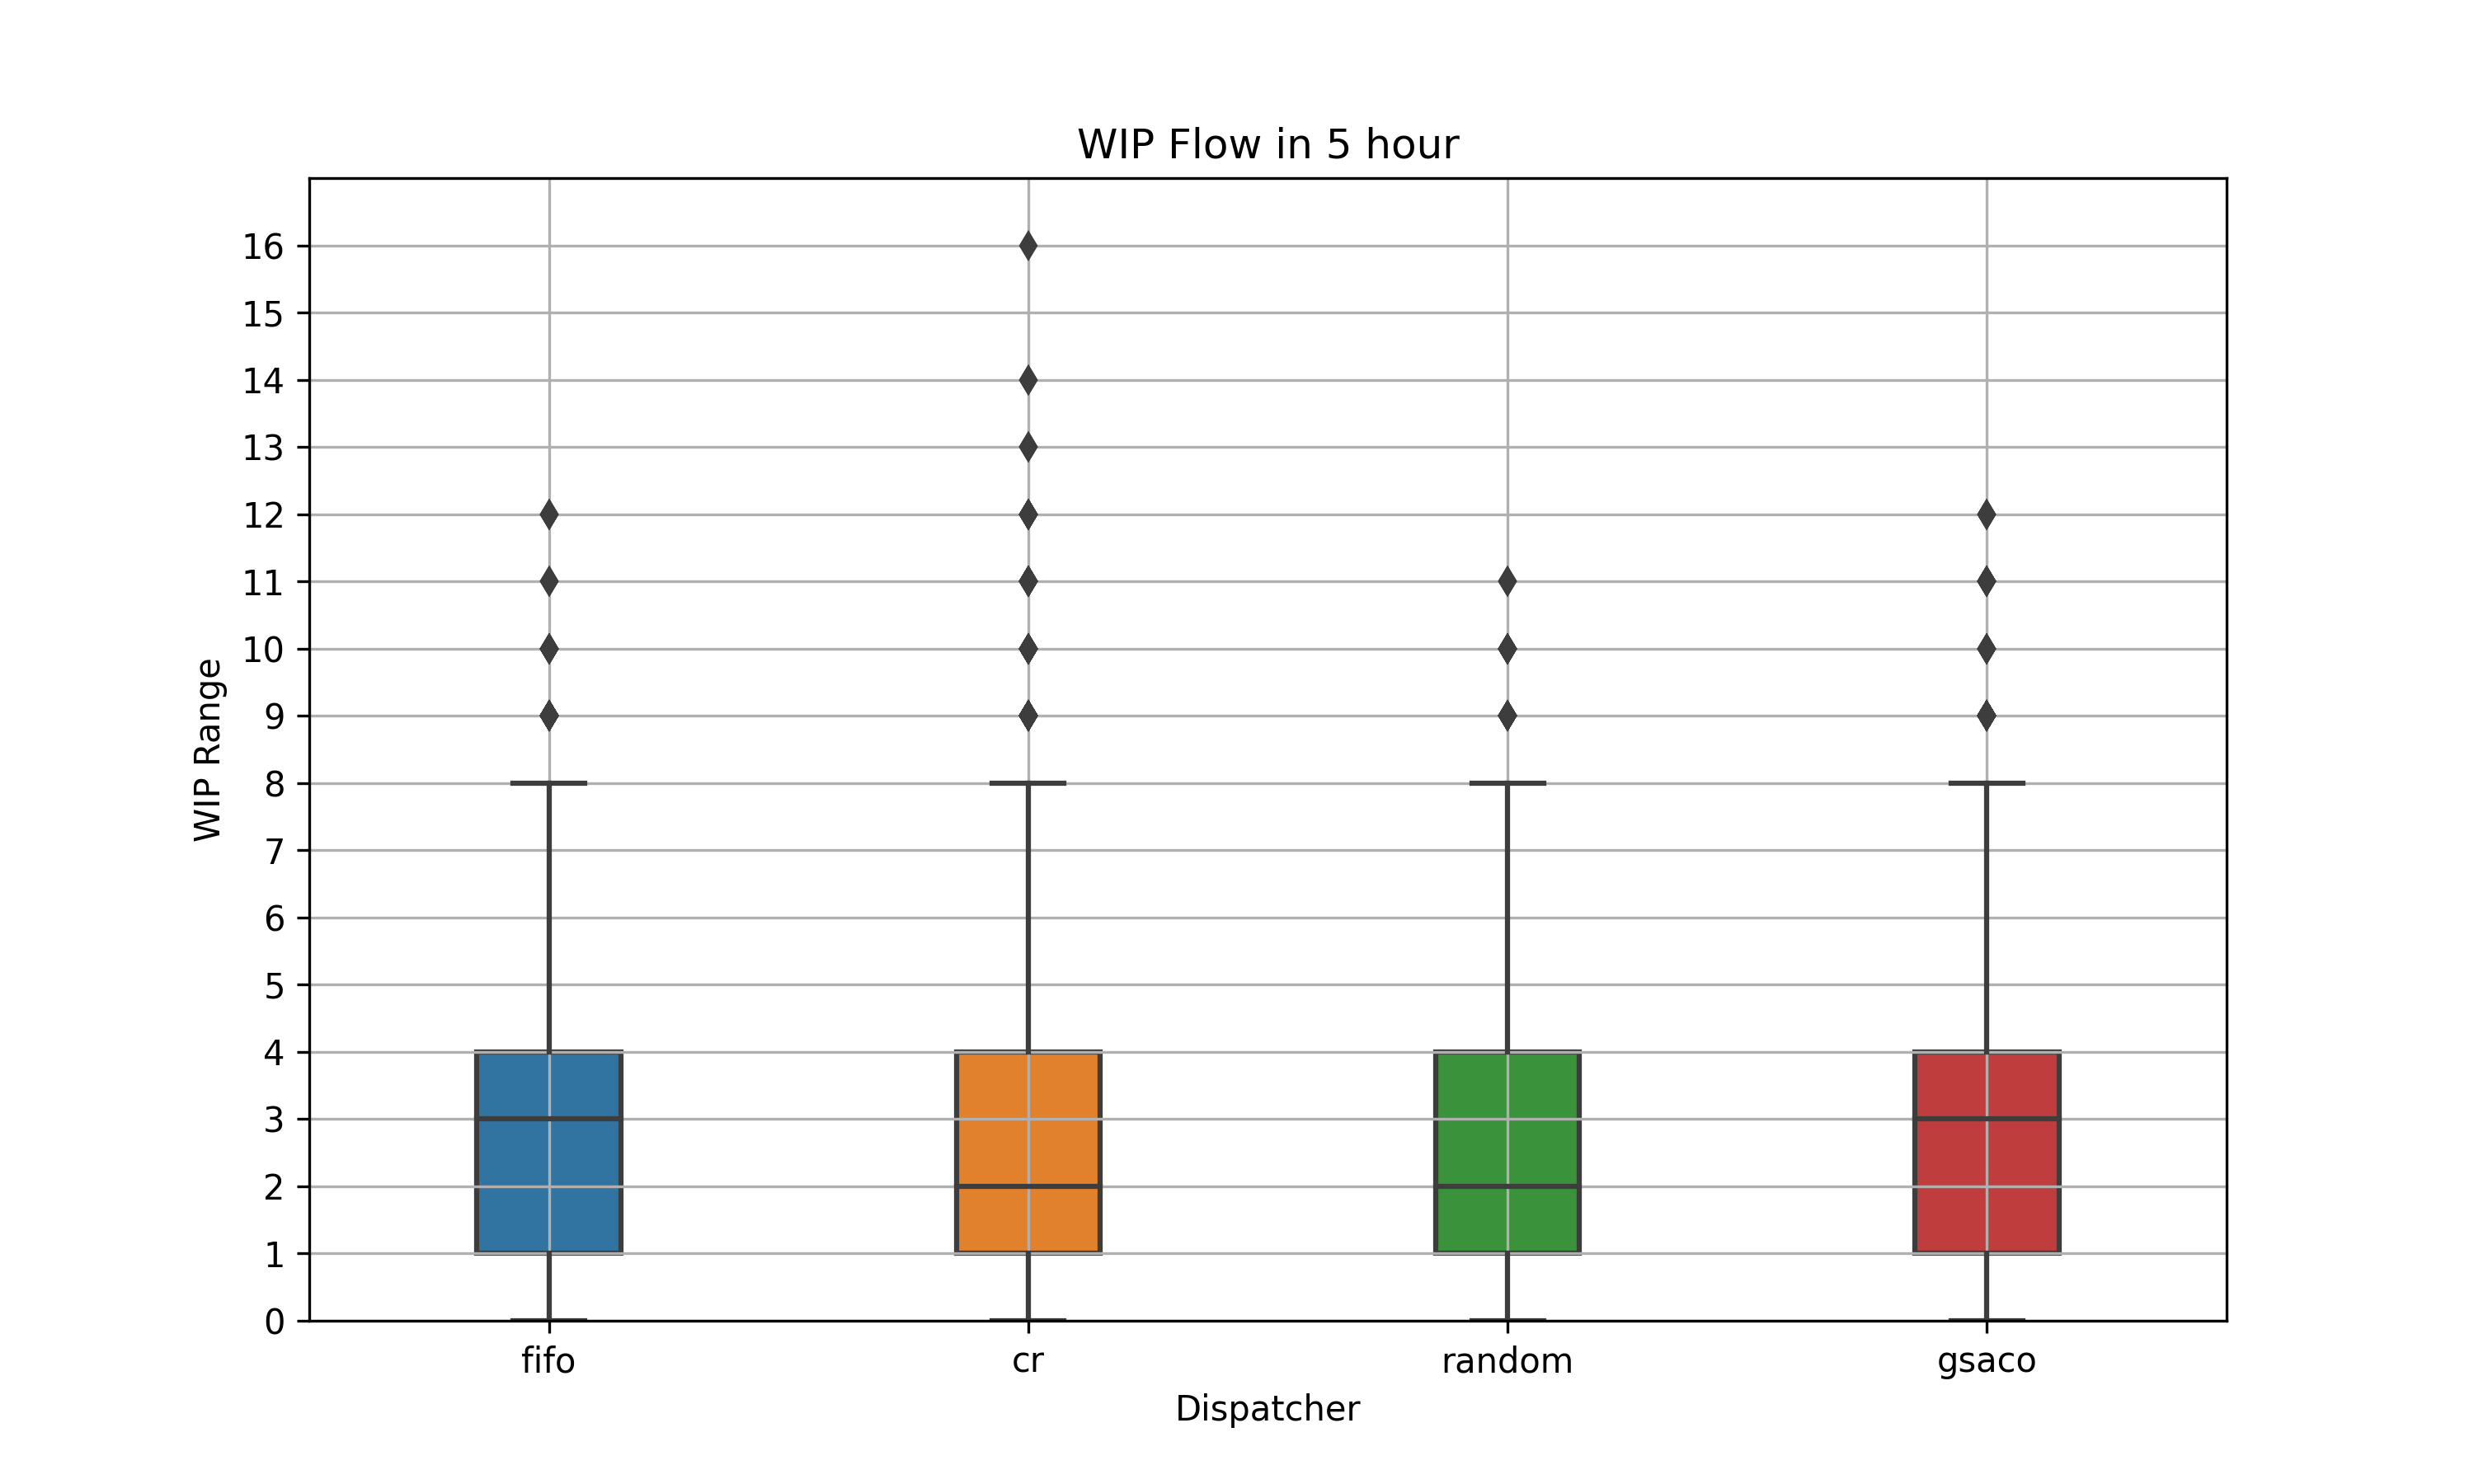
\includegraphics[width=\textwidth]{HVLM/period_18000s.png}
		% \caption{}
		% \label{fig:p5}
	\end{subfigure}
	\hfill
	\begin{subfigure}[b]{0.32\textwidth}
		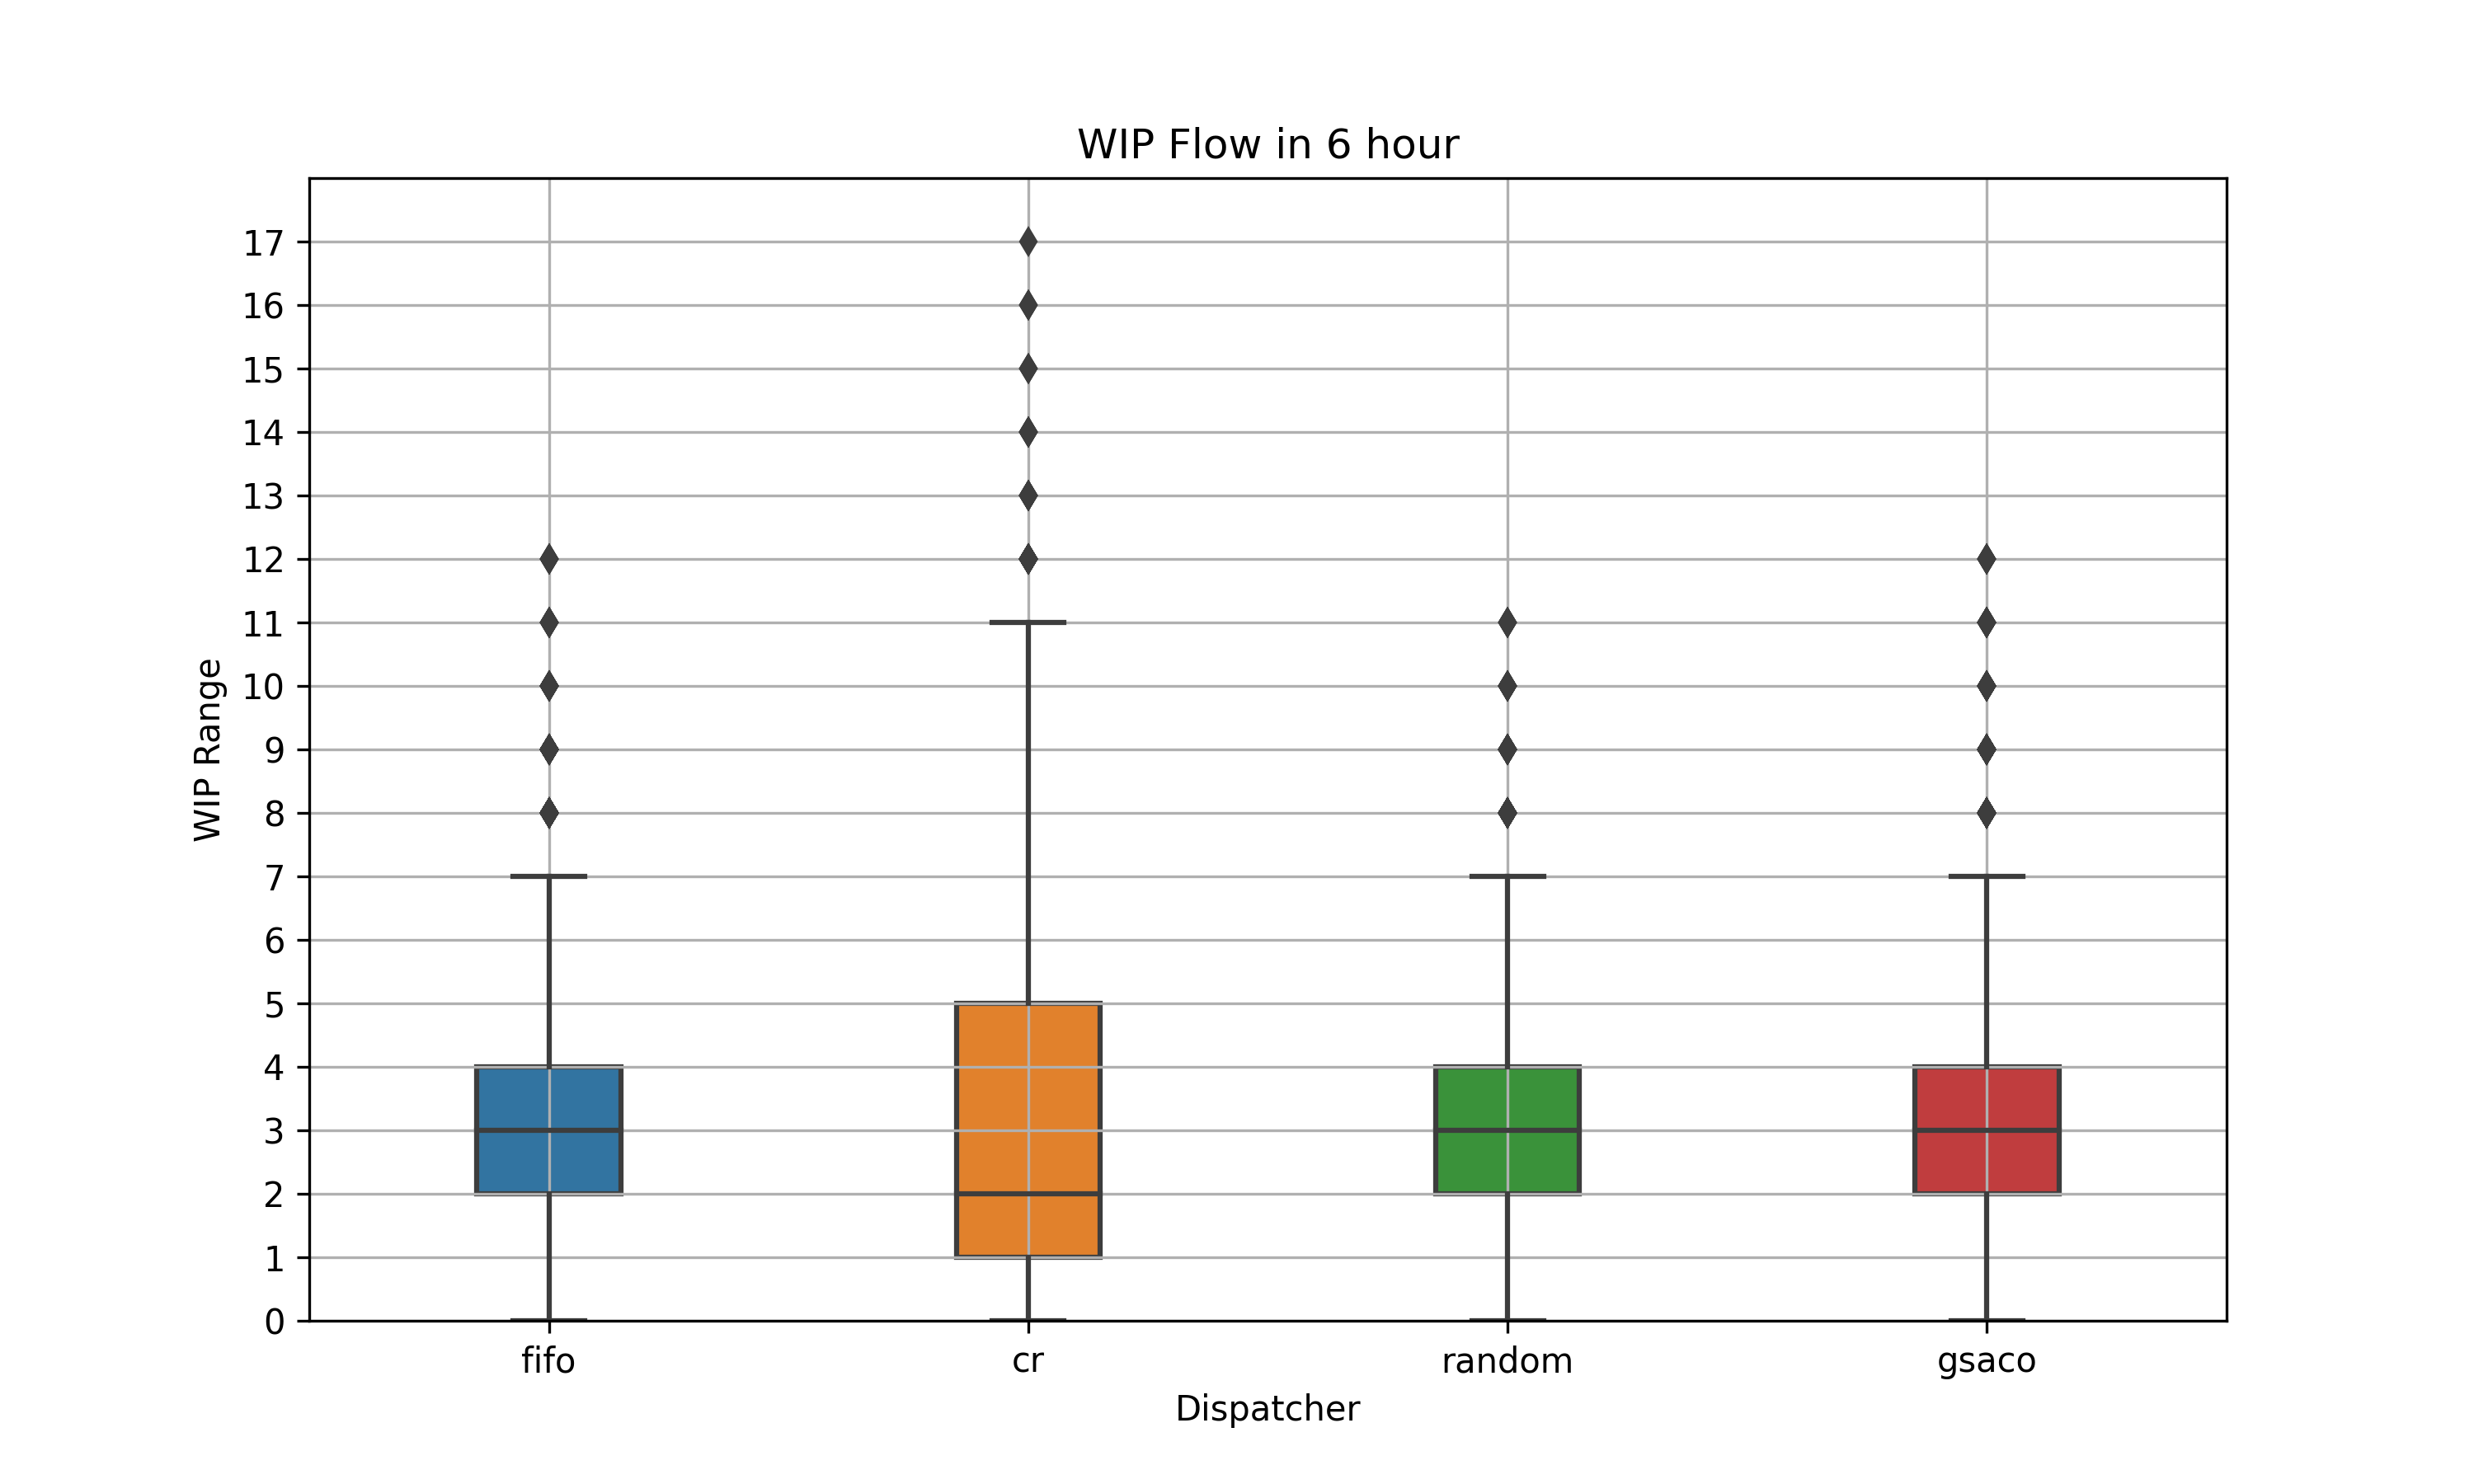
\includegraphics[width=\textwidth]{HVLM/period_21600s.png}
		% \caption{}
		% \label{fig:p6}
	\end{subfigure}
	\caption{WIP flow for HV/LM}
	\label{fig:wip-flows-HVLM}
\end{figure}

The plots in Figure~\ref{fig:totalopsHVLM} presents the performance of various dispatching rules—FIFO, CR, RANDOM, and GSACO—across different planning horizons ranging from 1 to 6 hours. Each plot illustrates the total number of operations dispatched by each rule within these time frames, offering a clear comparison of their efficiency and effectiveness in handling operational tasks within a semiconductor manufacturing.
\todo{M: Please unify the range of the $y$-scales in subfigures of each of the Figures~\ref{fig:totalopsHVLM}--\ref{fig:totalopsLVHM}.}

The performance of dispatching rules based on specific operational times and goals are analyzed. While simpler rules like FIFO and CR are predictable and may perform adequately in stable environments, their performance can lag in more dynamic or complex scenarios where adaptive strategies like GSACO provide significant advantages. Random dispatching, surprisingly effective in some cases, suggests that stochastic elements might occasionally align with operational demands, although this method's reliability is less consistent. GSACO's consistently superior performance advocates for its use in environments where maximizing operational throughput is critical. This analysis not only aids in strategic decision-making but also highlights the potential for further refining these algorithms to enhance their applicability and effectiveness across various manufacturing contexts.

The plots in Figure~\ref{fig:wip-flows-HVLM} illustrate the Work in Progress (WIP) flow across various dispatching rules—FIFO, CR, RANDOM, and GSACO —over different planning horizons ranging from 1 to 6 hours. Each bar demonstrates the minimum and maximum WIP levels reached during the simulation period under each dispatching rule, with the height of the bar indicating the variability or stability of the WIP flow.

FIFO shows the lowest range of WIP variability, suggesting consistent and predictable processing under this rule within the first hour. CR and Random display slightly higher variability, indicating a less stable WIP flow.
GSACO exhibits the highest range, potentially due to more aggressive reordering and optimization strategies that initially increase variability before stabilizing.

As the planning horizon extends to 2, 3, 4, 5, and 6 hours, all methods show an increase in the maximum WIP range. FIFO consistently maintains a relatively lower range of WIP compared to other methods, indicating its less dynamic but stable approach.
CR's performance exhibits moderate variability, reflecting its strategy of prioritizing jobs based on their deadlines, which might not always align with minimizing WIP.
Random shows a moderate to high variability, which aligns with its inherent unpredictability.
GSACO consistently demonstrates the highest variability. This could be attributed to its optimization processes, which might involve significant shifts in job prioritization and scheduling to achieve long-term efficiency, leading to larger fluctuations in WIP.

\begin{figure}[t]
	\centering
	\begin{subfigure}{0.32\textwidth}
		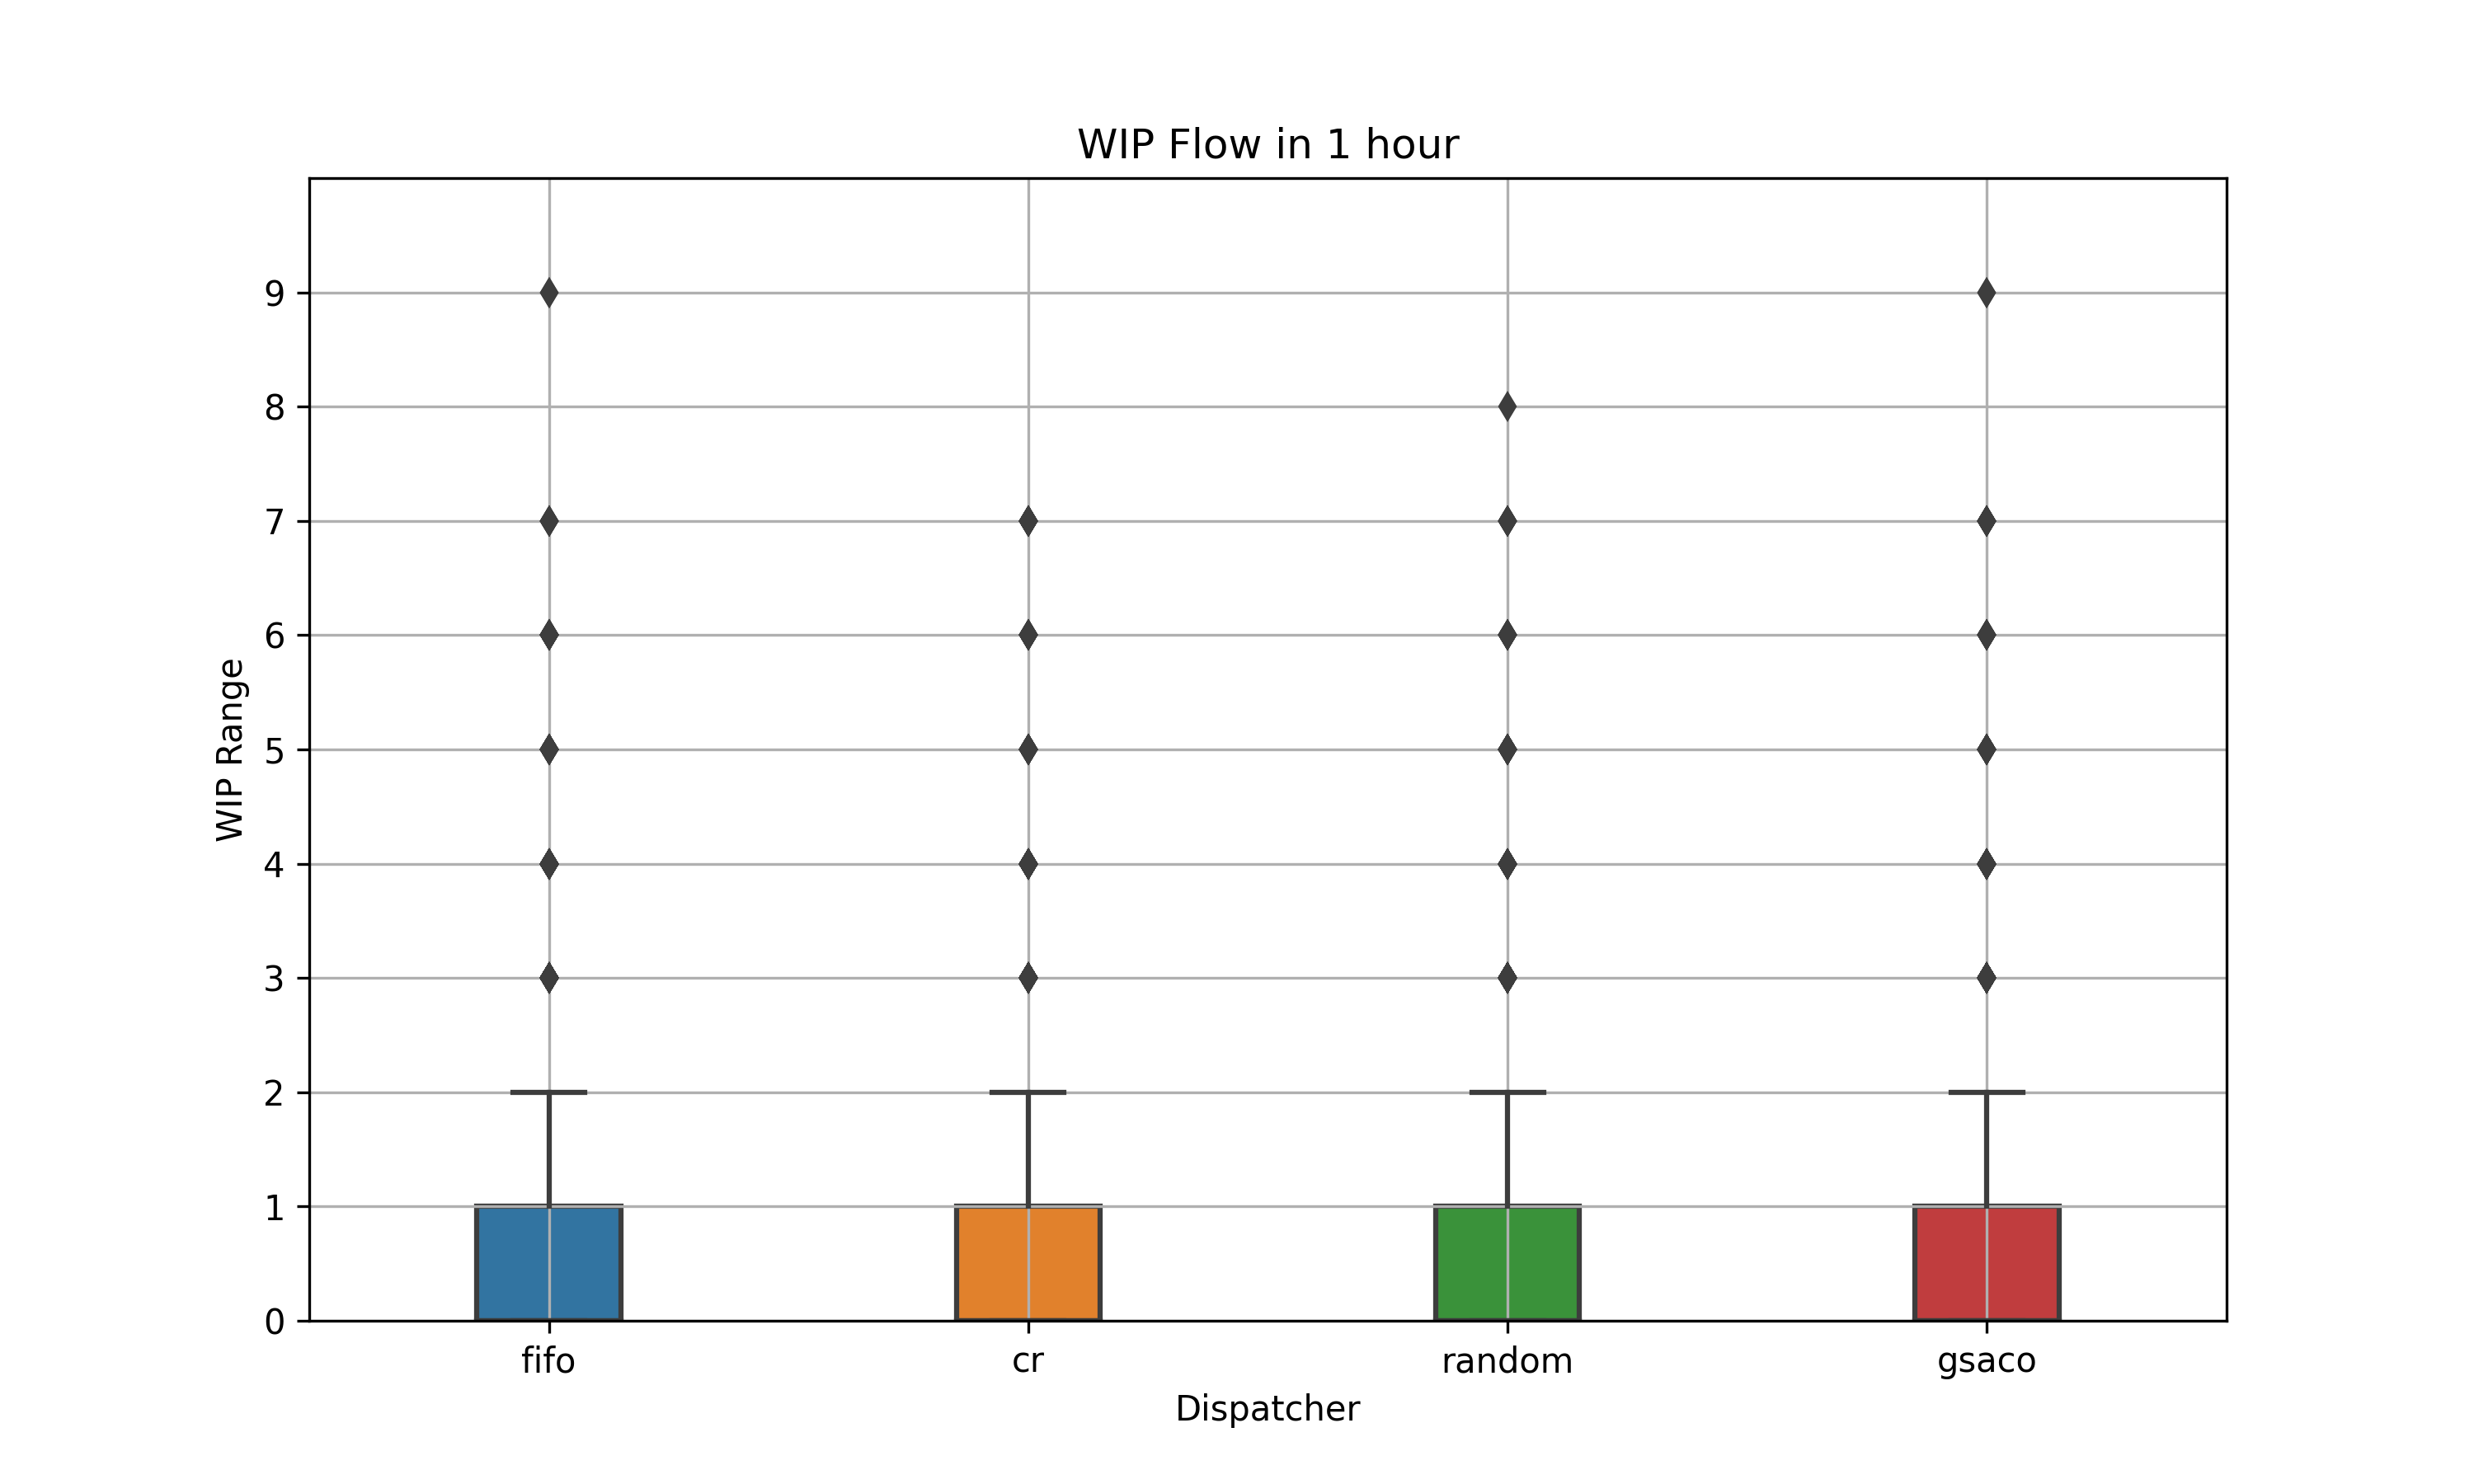
\includegraphics[width=\textwidth]{LVHM/period_3600s.png}
		% \caption{}
		% \label{fig:pp1}
	\end{subfigure}\hfill
	\begin{subfigure}{0.32\textwidth}
		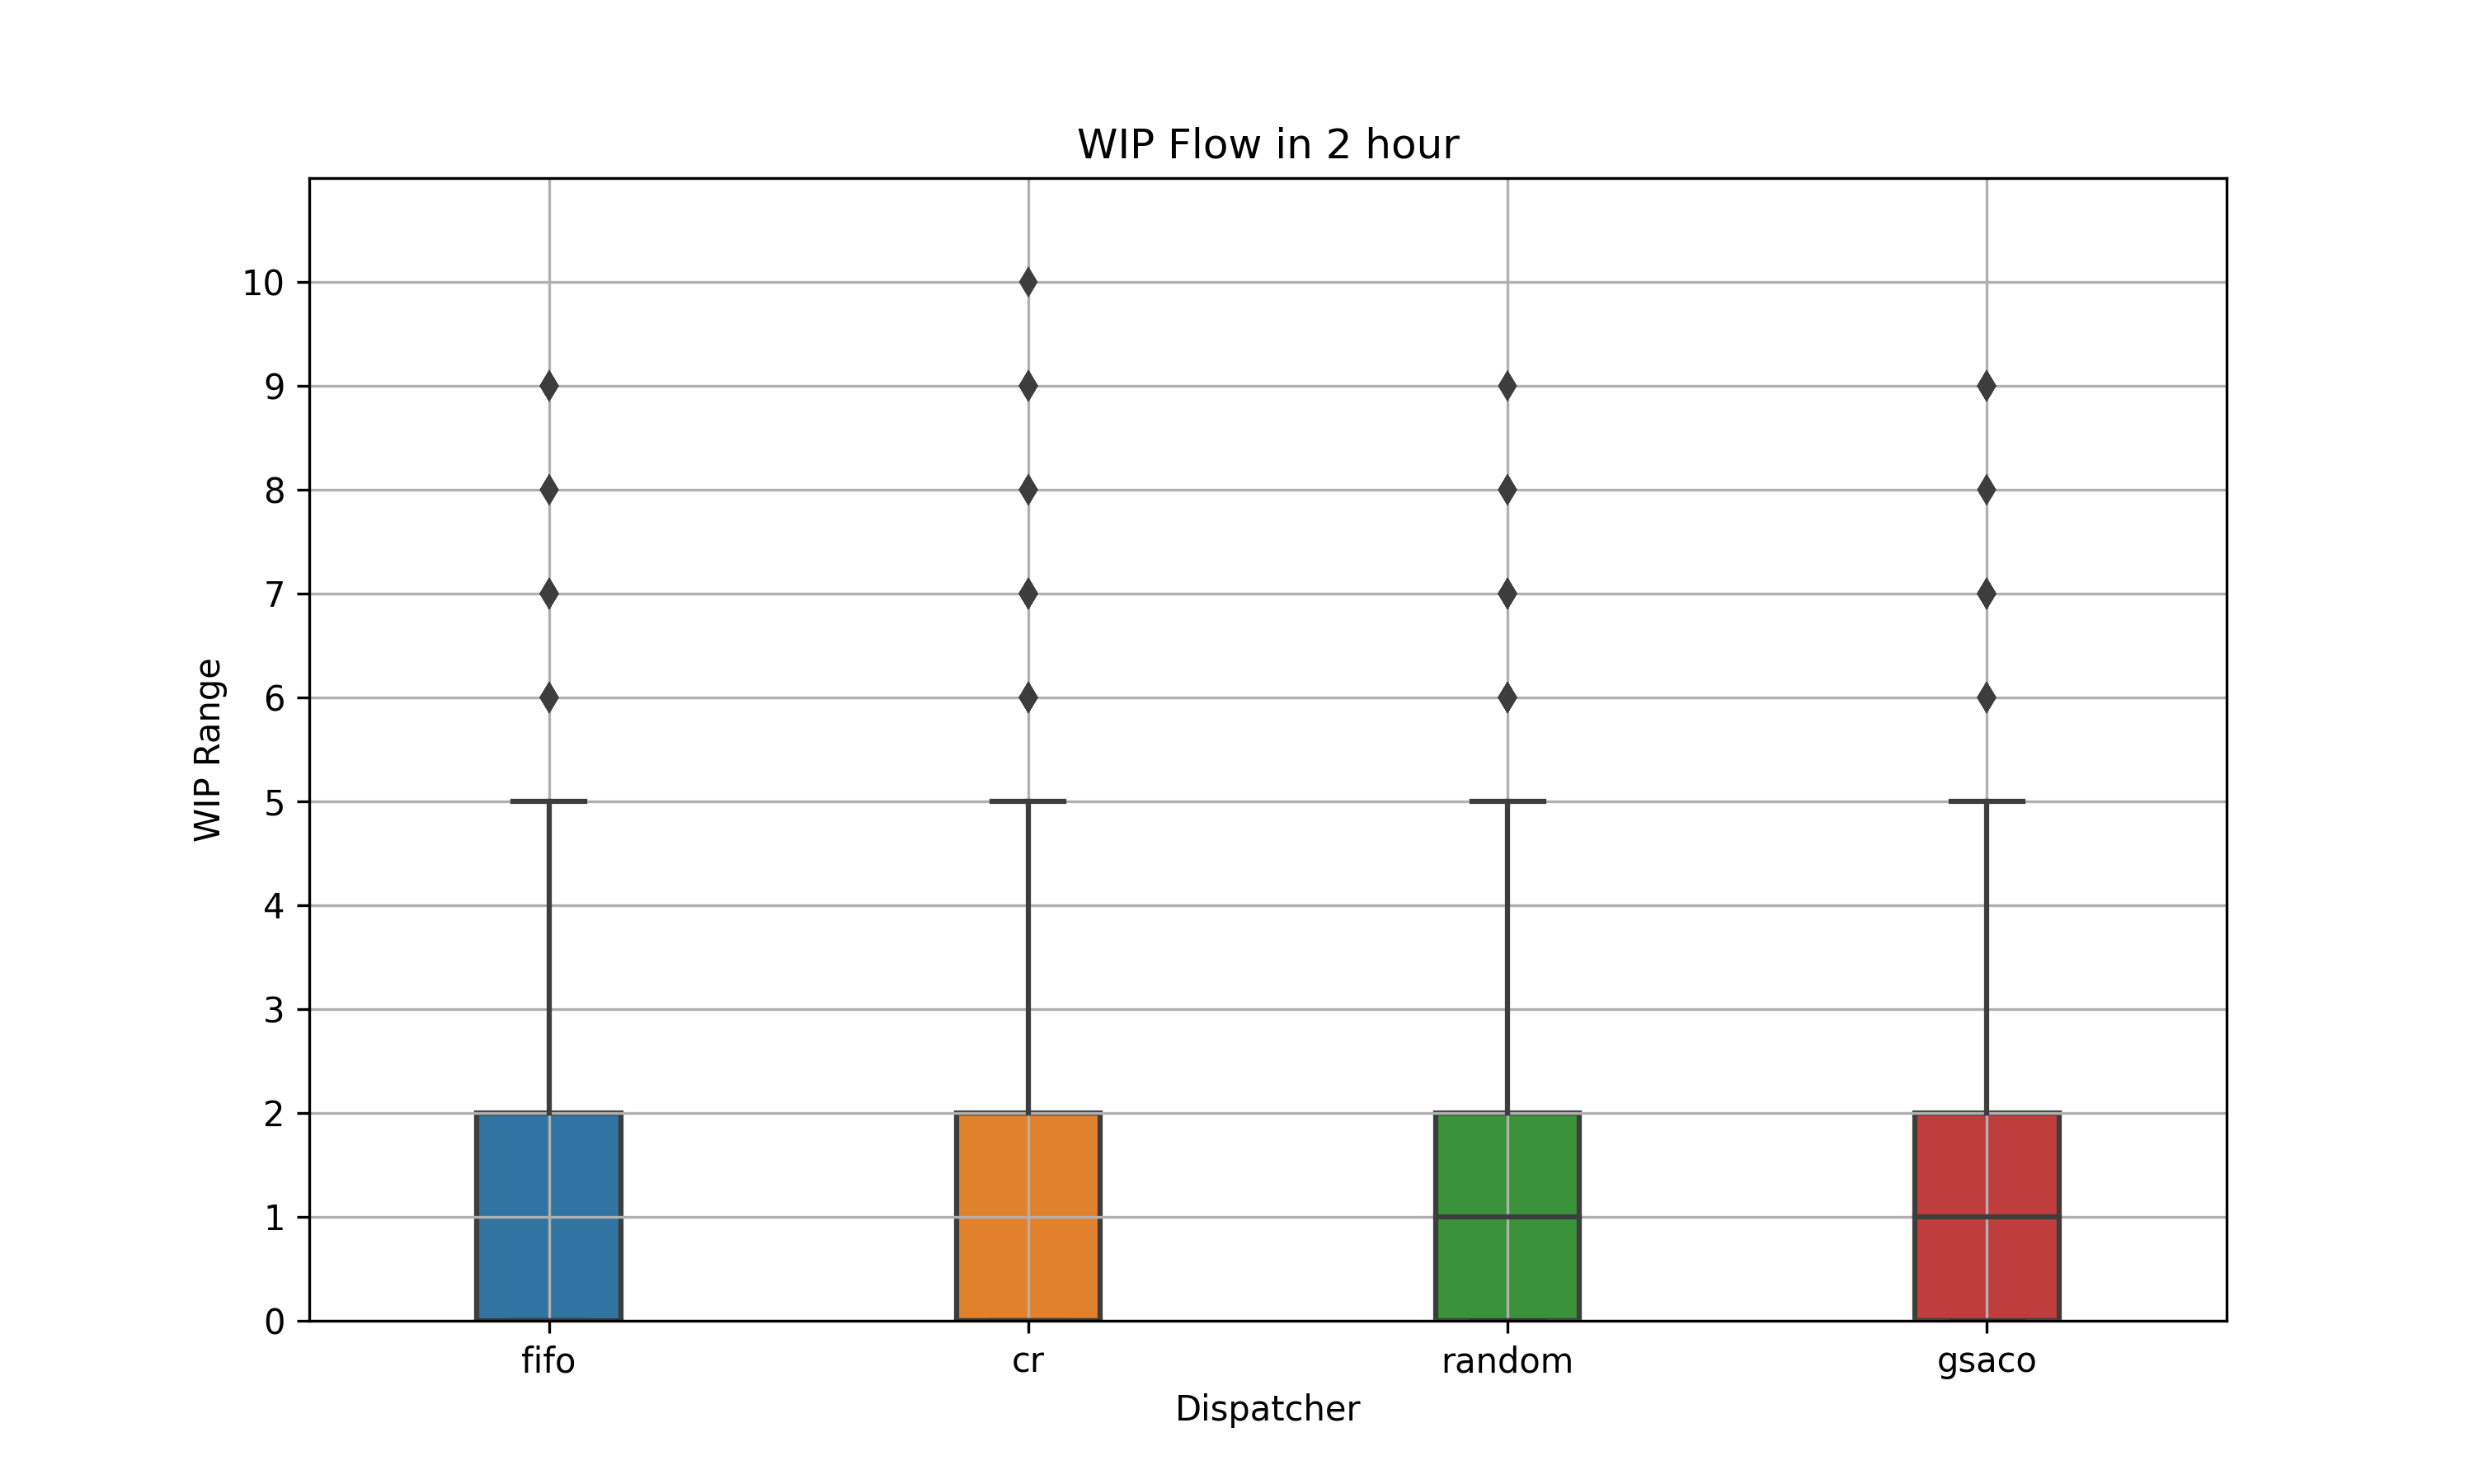
\includegraphics[width=\textwidth]{LVHM/period_7200s.png}
		% \caption{}
		% \label{fig:pp2}
	\end{subfigure}\hfill
	\begin{subfigure}{0.32\textwidth}
		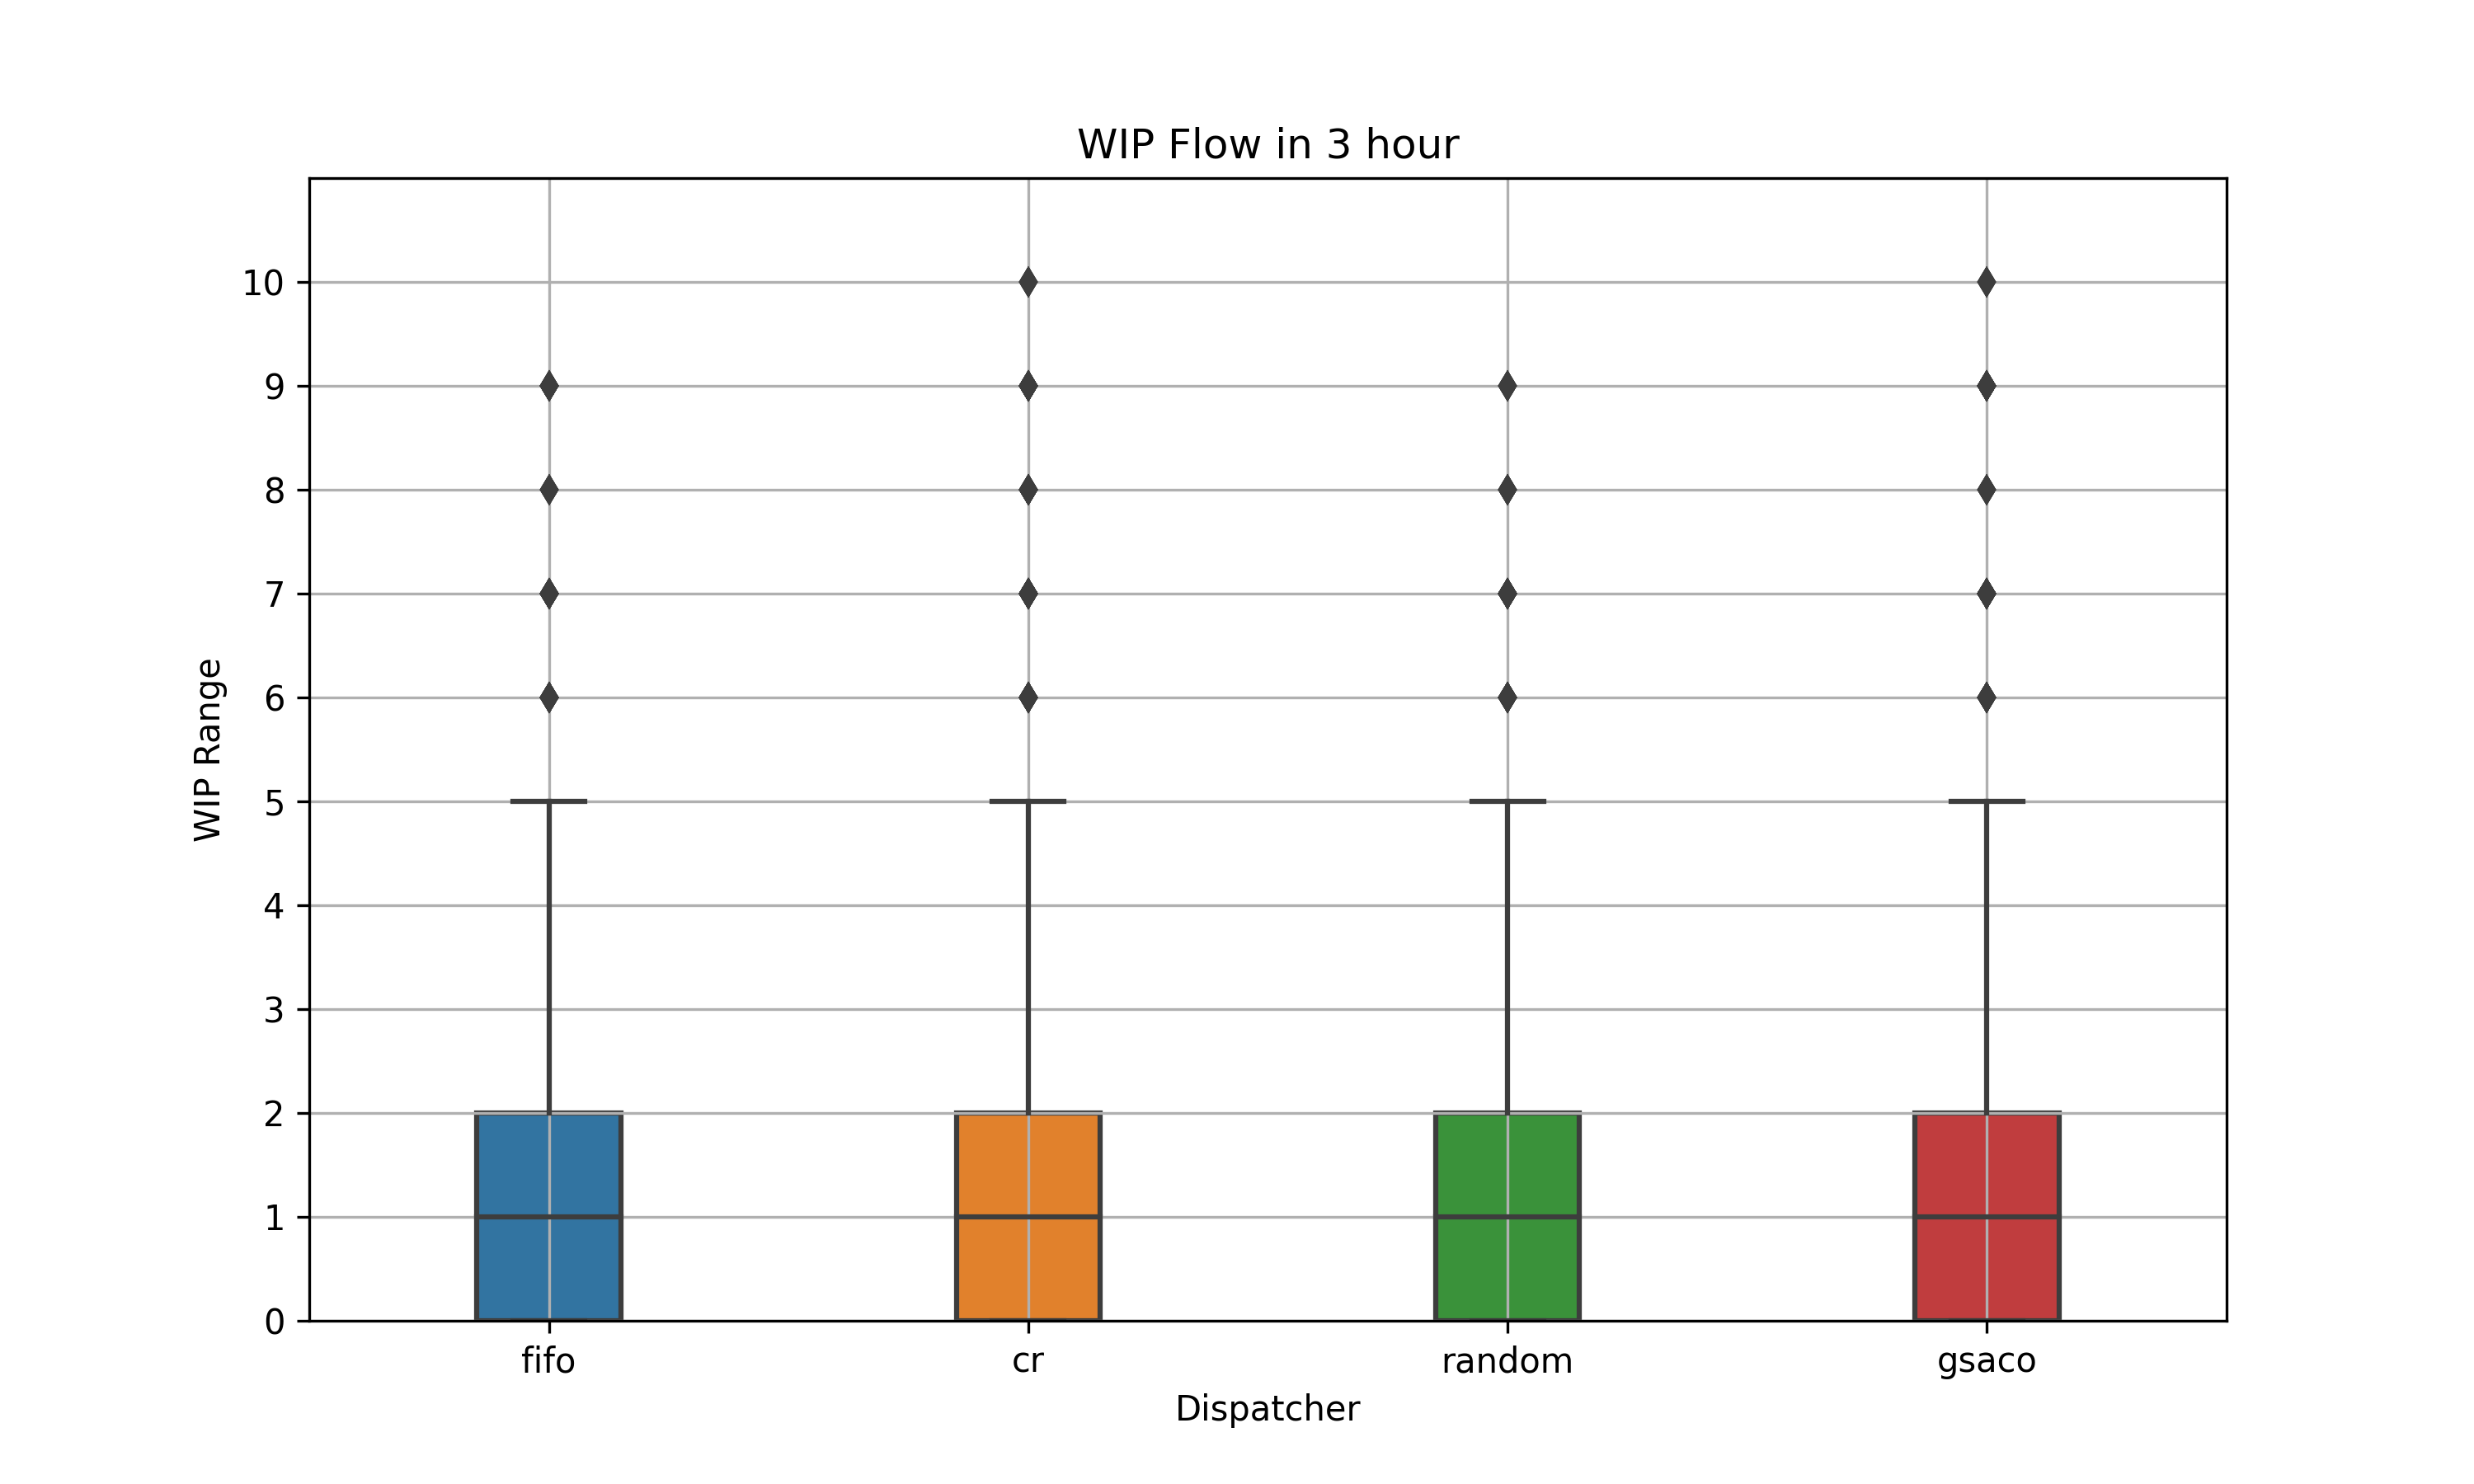
\includegraphics[width=\textwidth]{LVHM/period_10800s.png}
		% \caption{}
		% \label{fig:pp3}
	\end{subfigure}
	\begin{subfigure}{0.32\textwidth}
		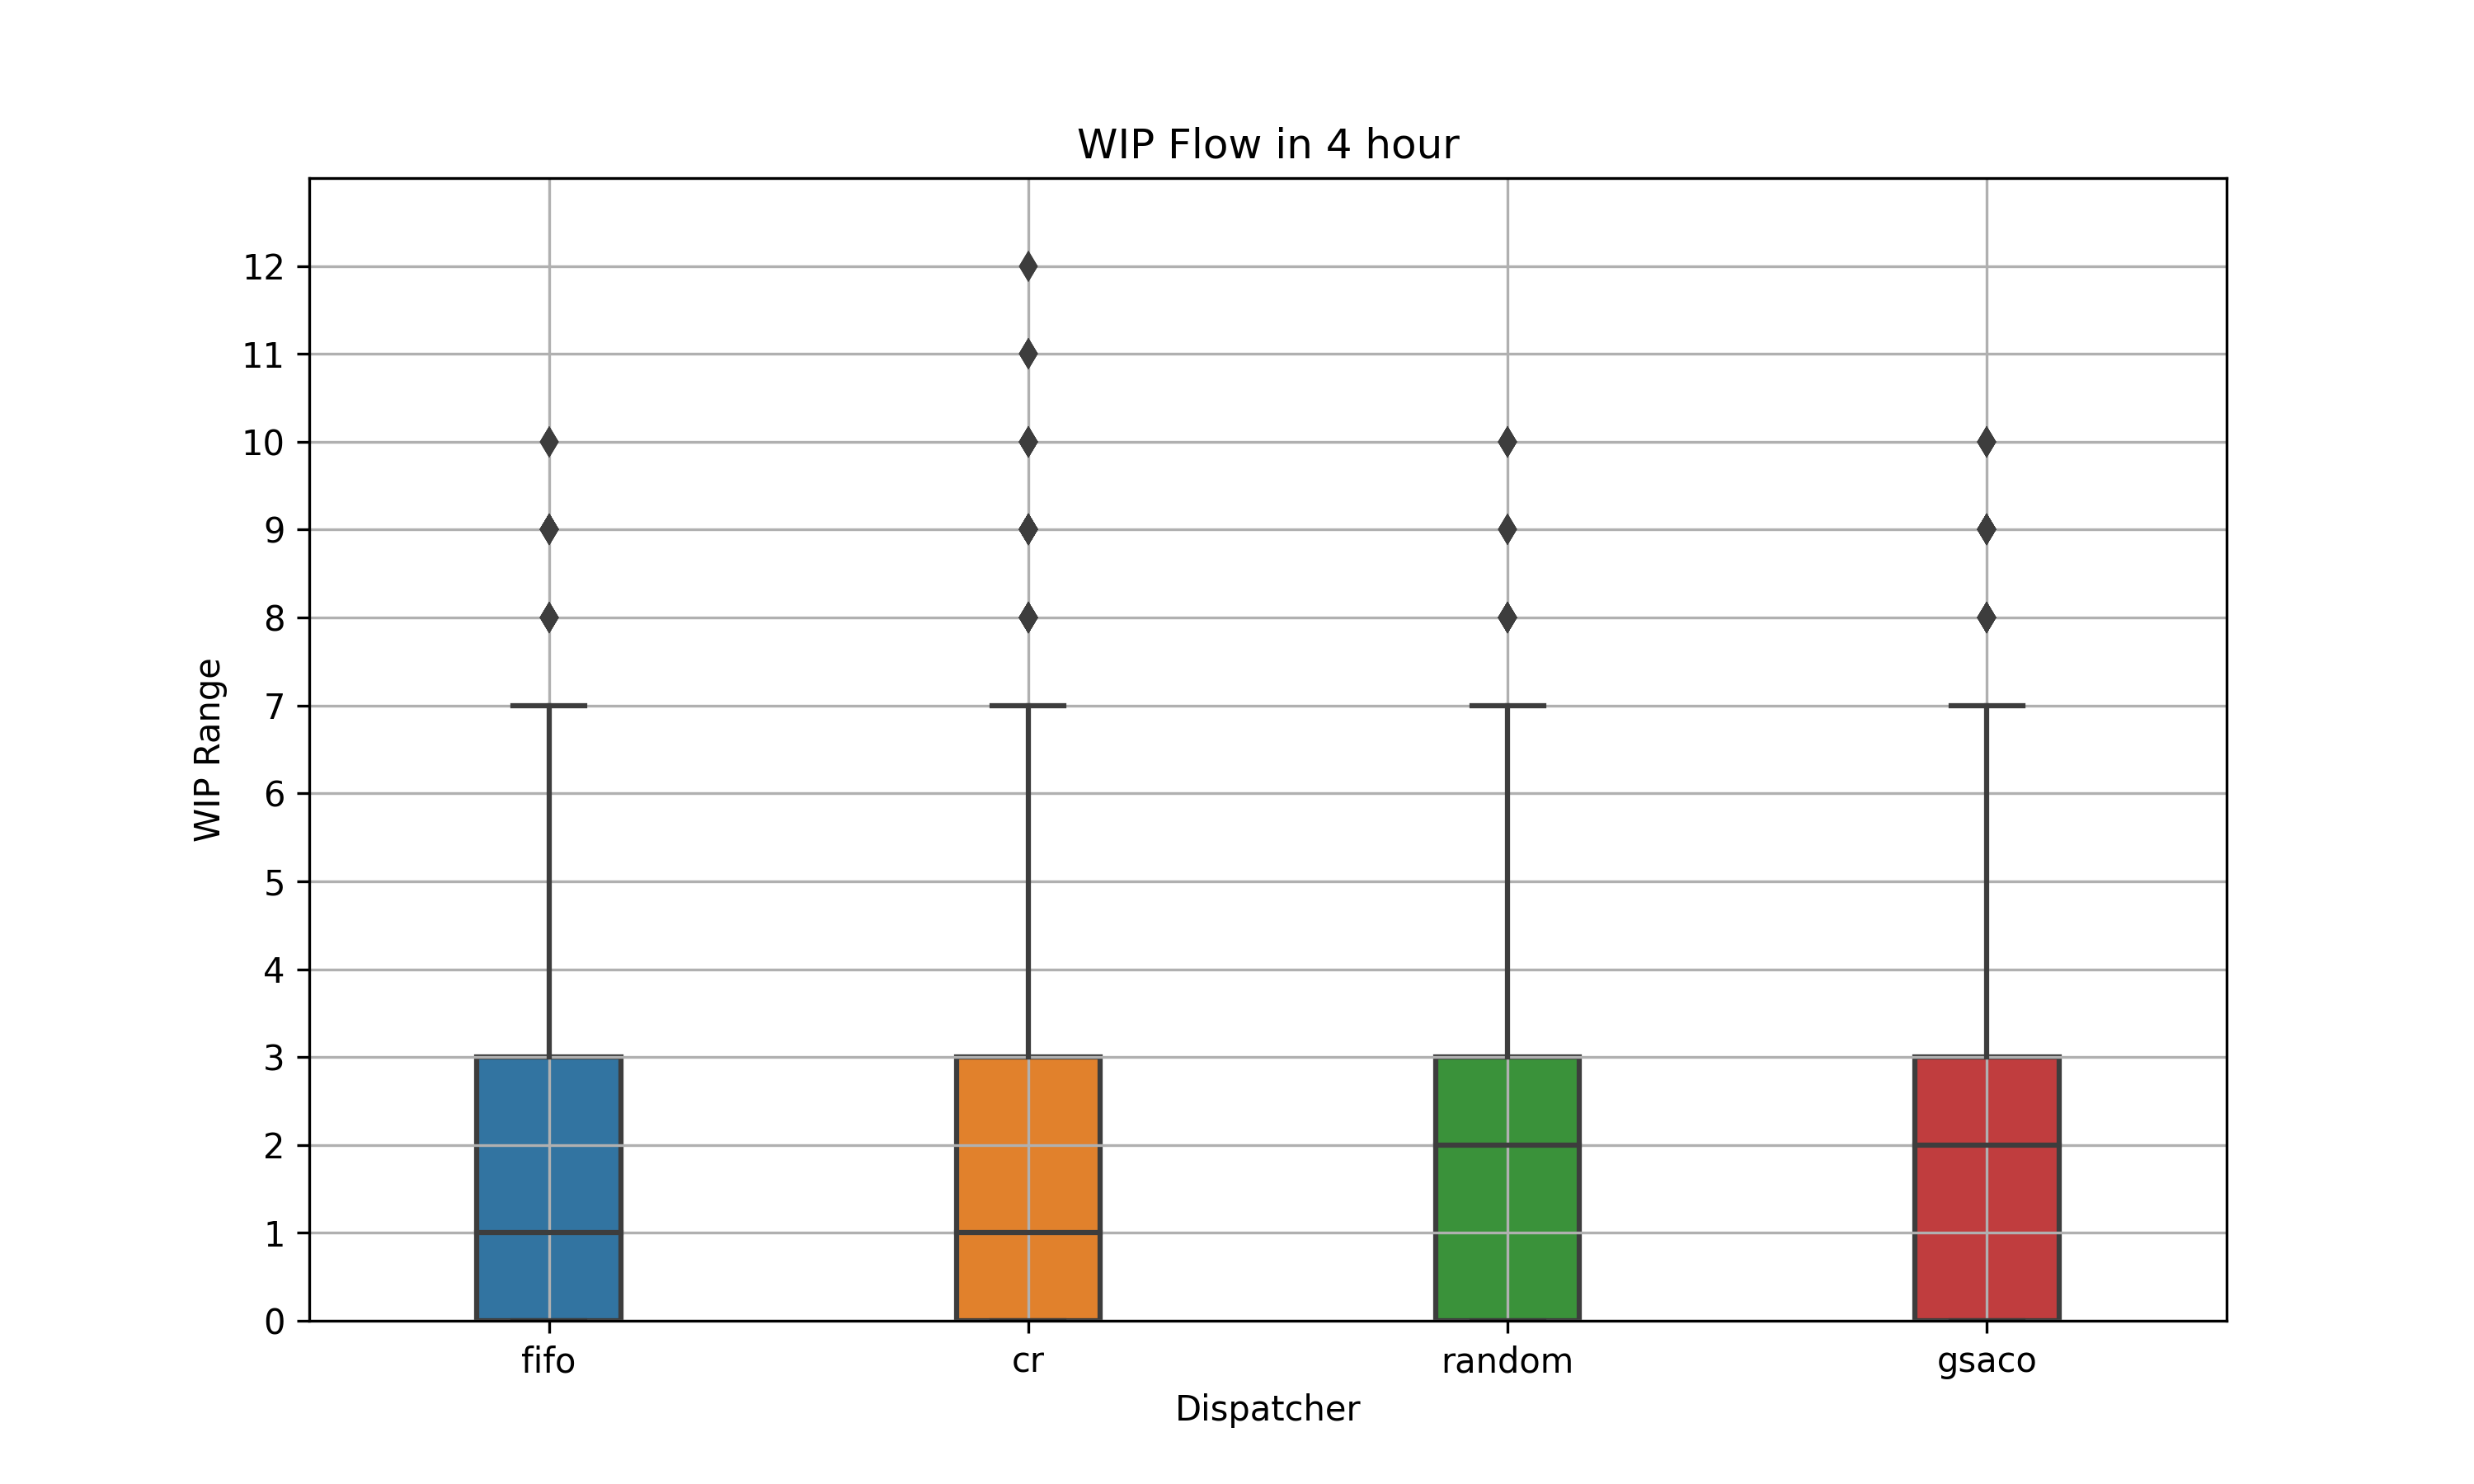
\includegraphics[width=\textwidth]{LVHM/period_14400s.png}
		% \caption{}
		% \label{fig:pp4}
	\end{subfigure}\hfill
	\begin{subfigure}{0.32\textwidth}
		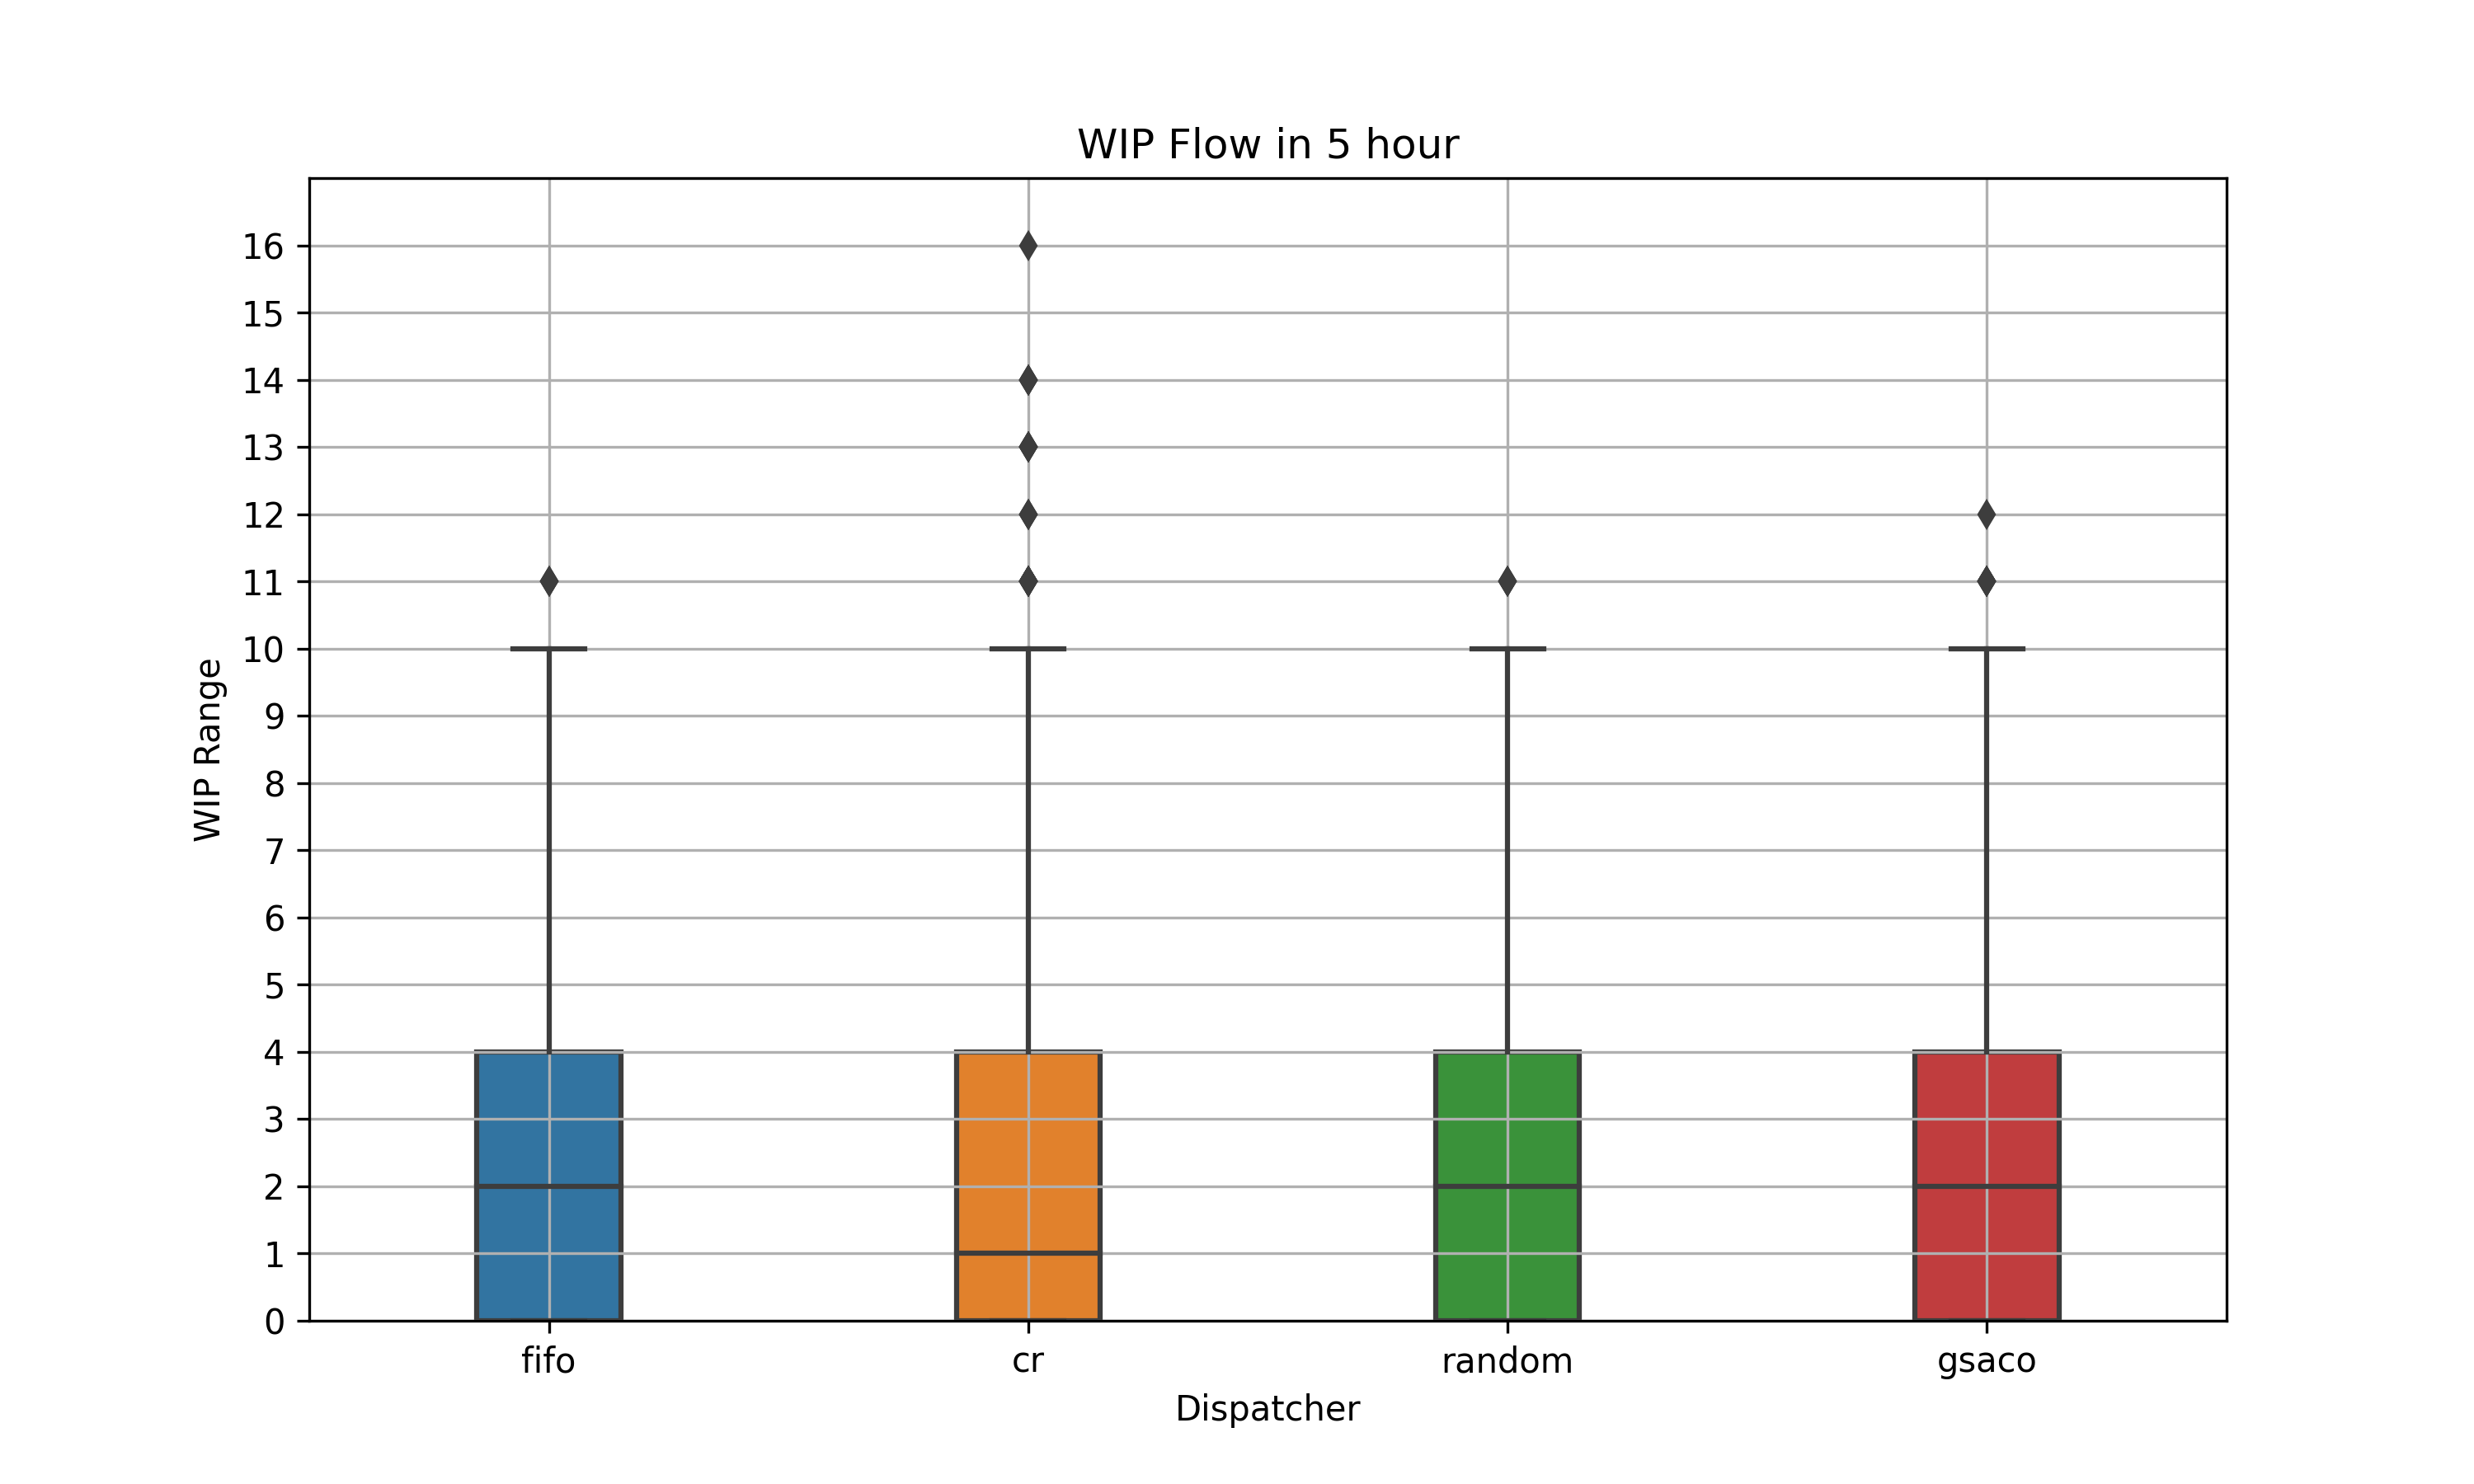
\includegraphics[width=\textwidth]{LVHM/period_18000s.png}
		% \caption{}
		% \label{fig:pp5}
	\end{subfigure}\hfill
	\begin{subfigure}{0.32\textwidth}
		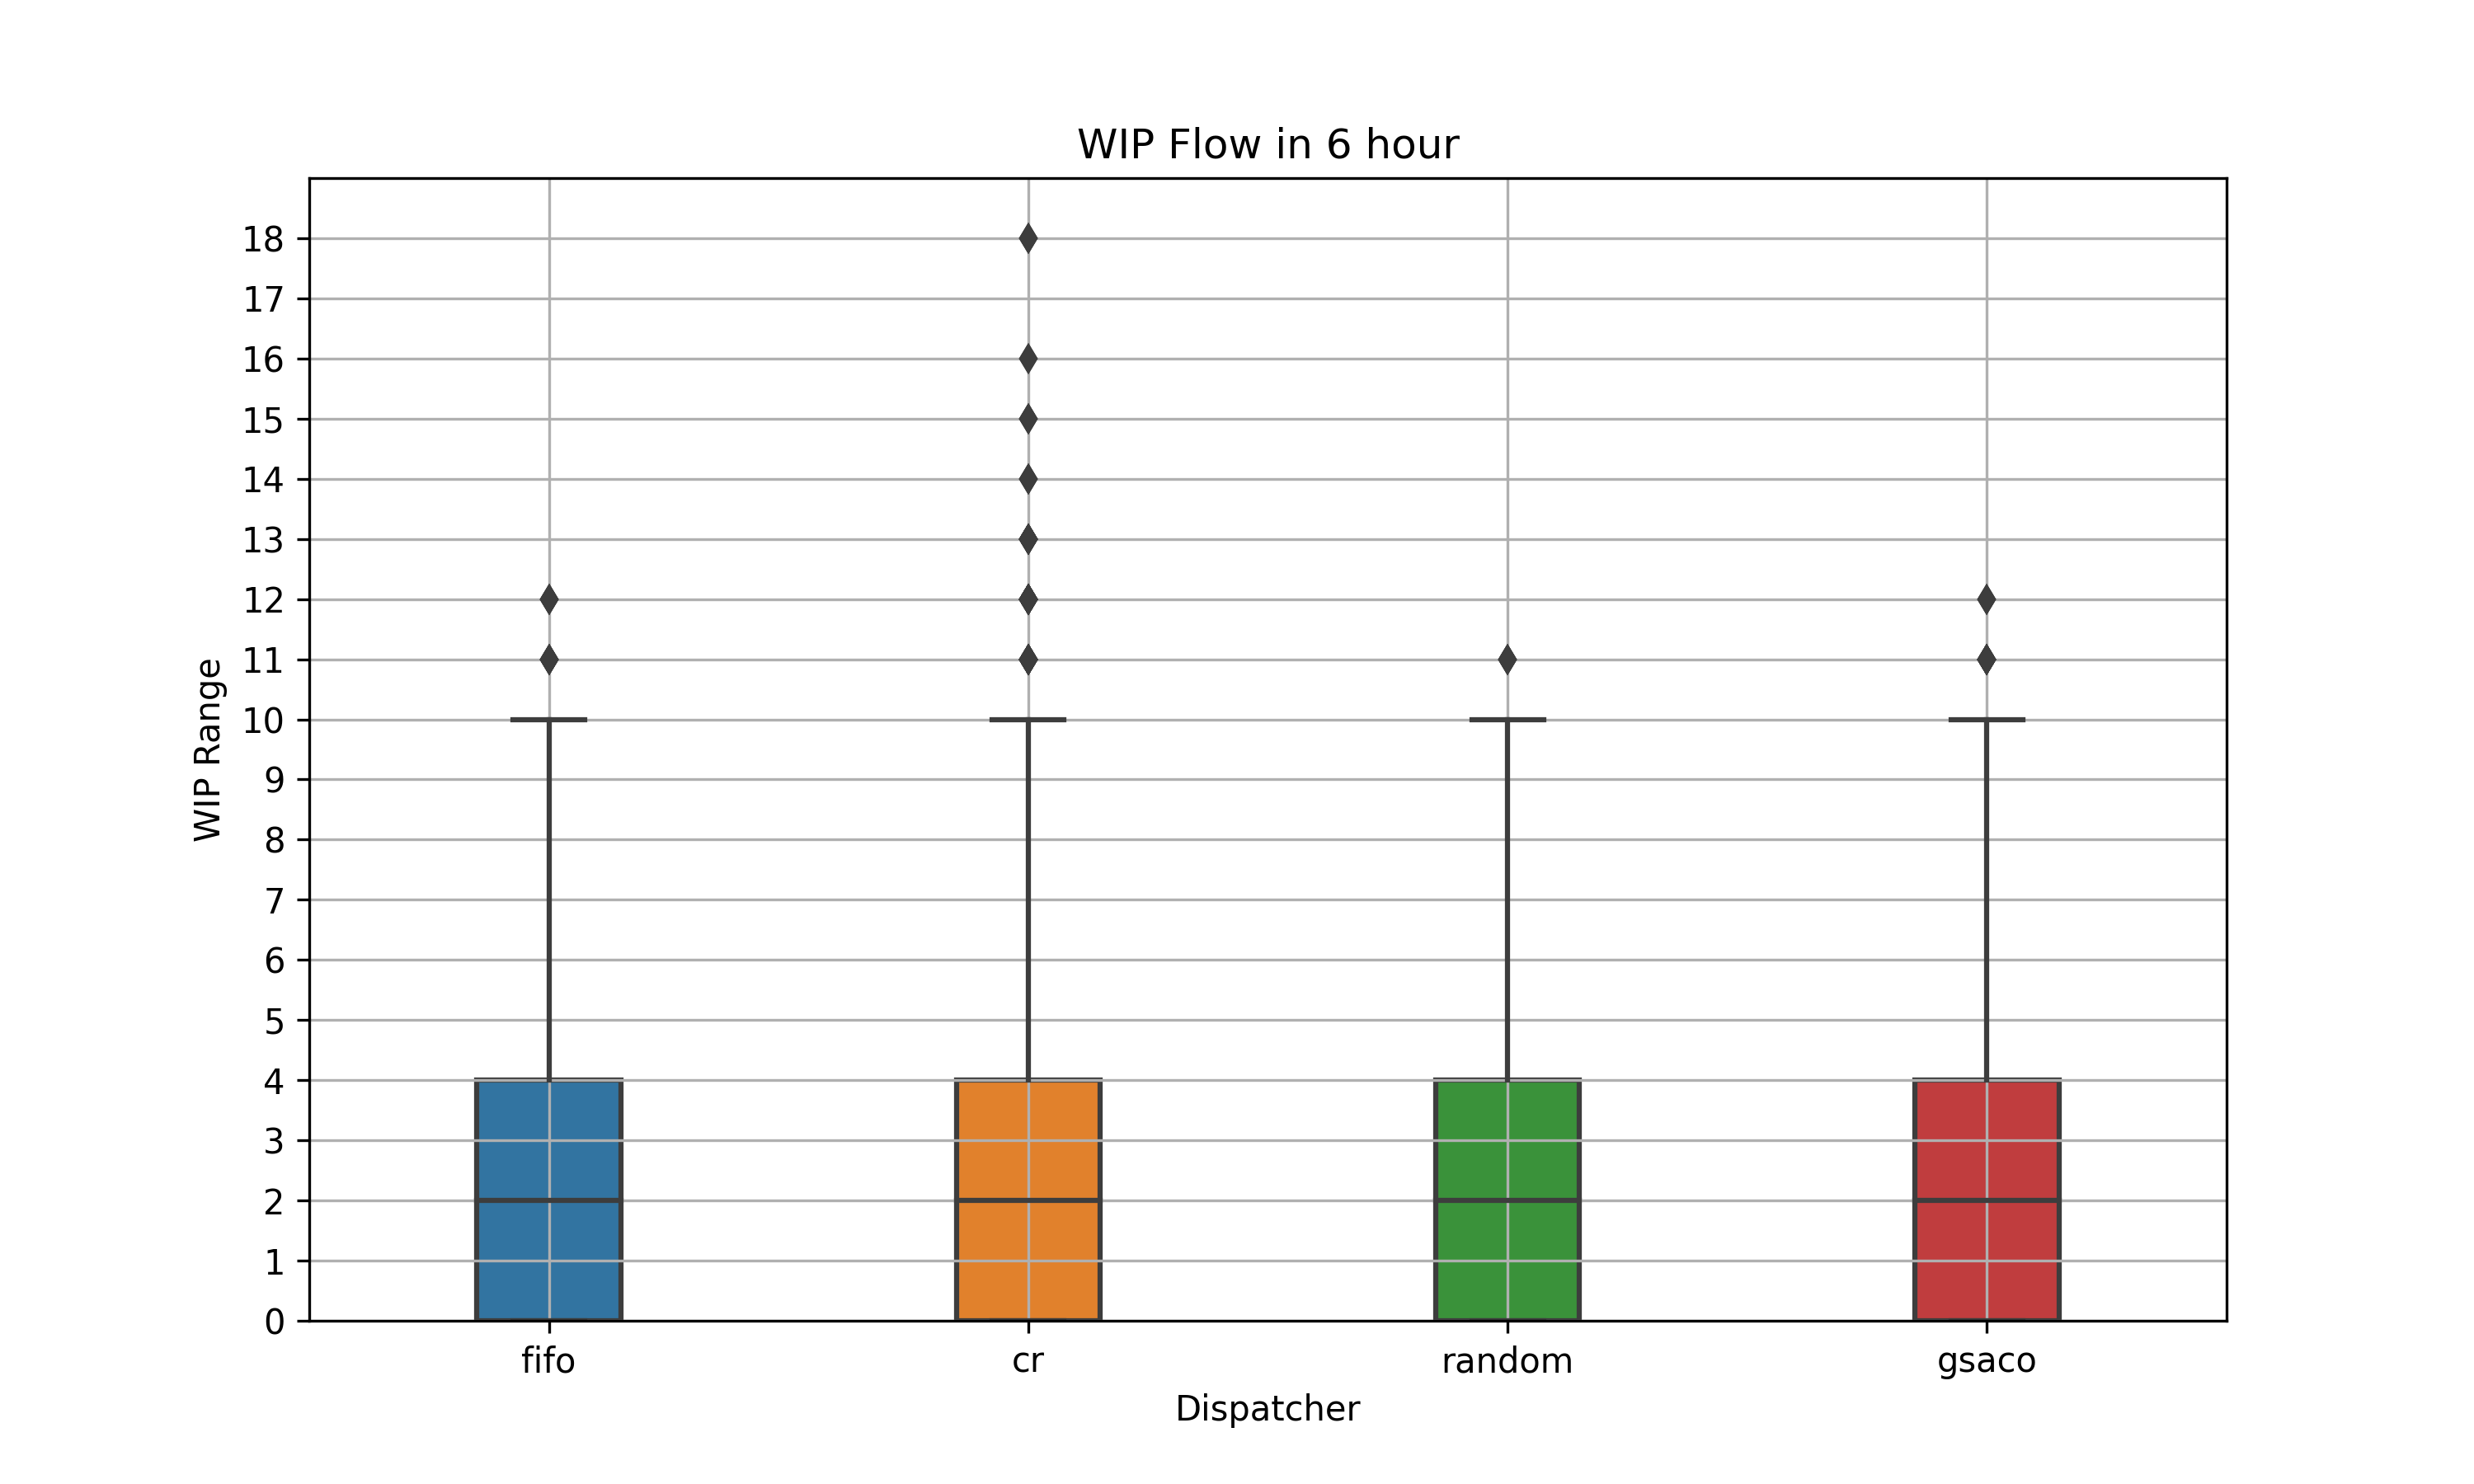
\includegraphics[width=\textwidth]{LVHM/period_21600s.png}
		% \caption{}
		% \label{fig:pp6}
	\end{subfigure}
    \caption{WIP flow for LV/HM}
    \label{fig:wip-flows-LVHM}
\end{figure}


\begin{figure}[ht]
	\centering
	\begin{subfigure}{0.32\textwidth}
		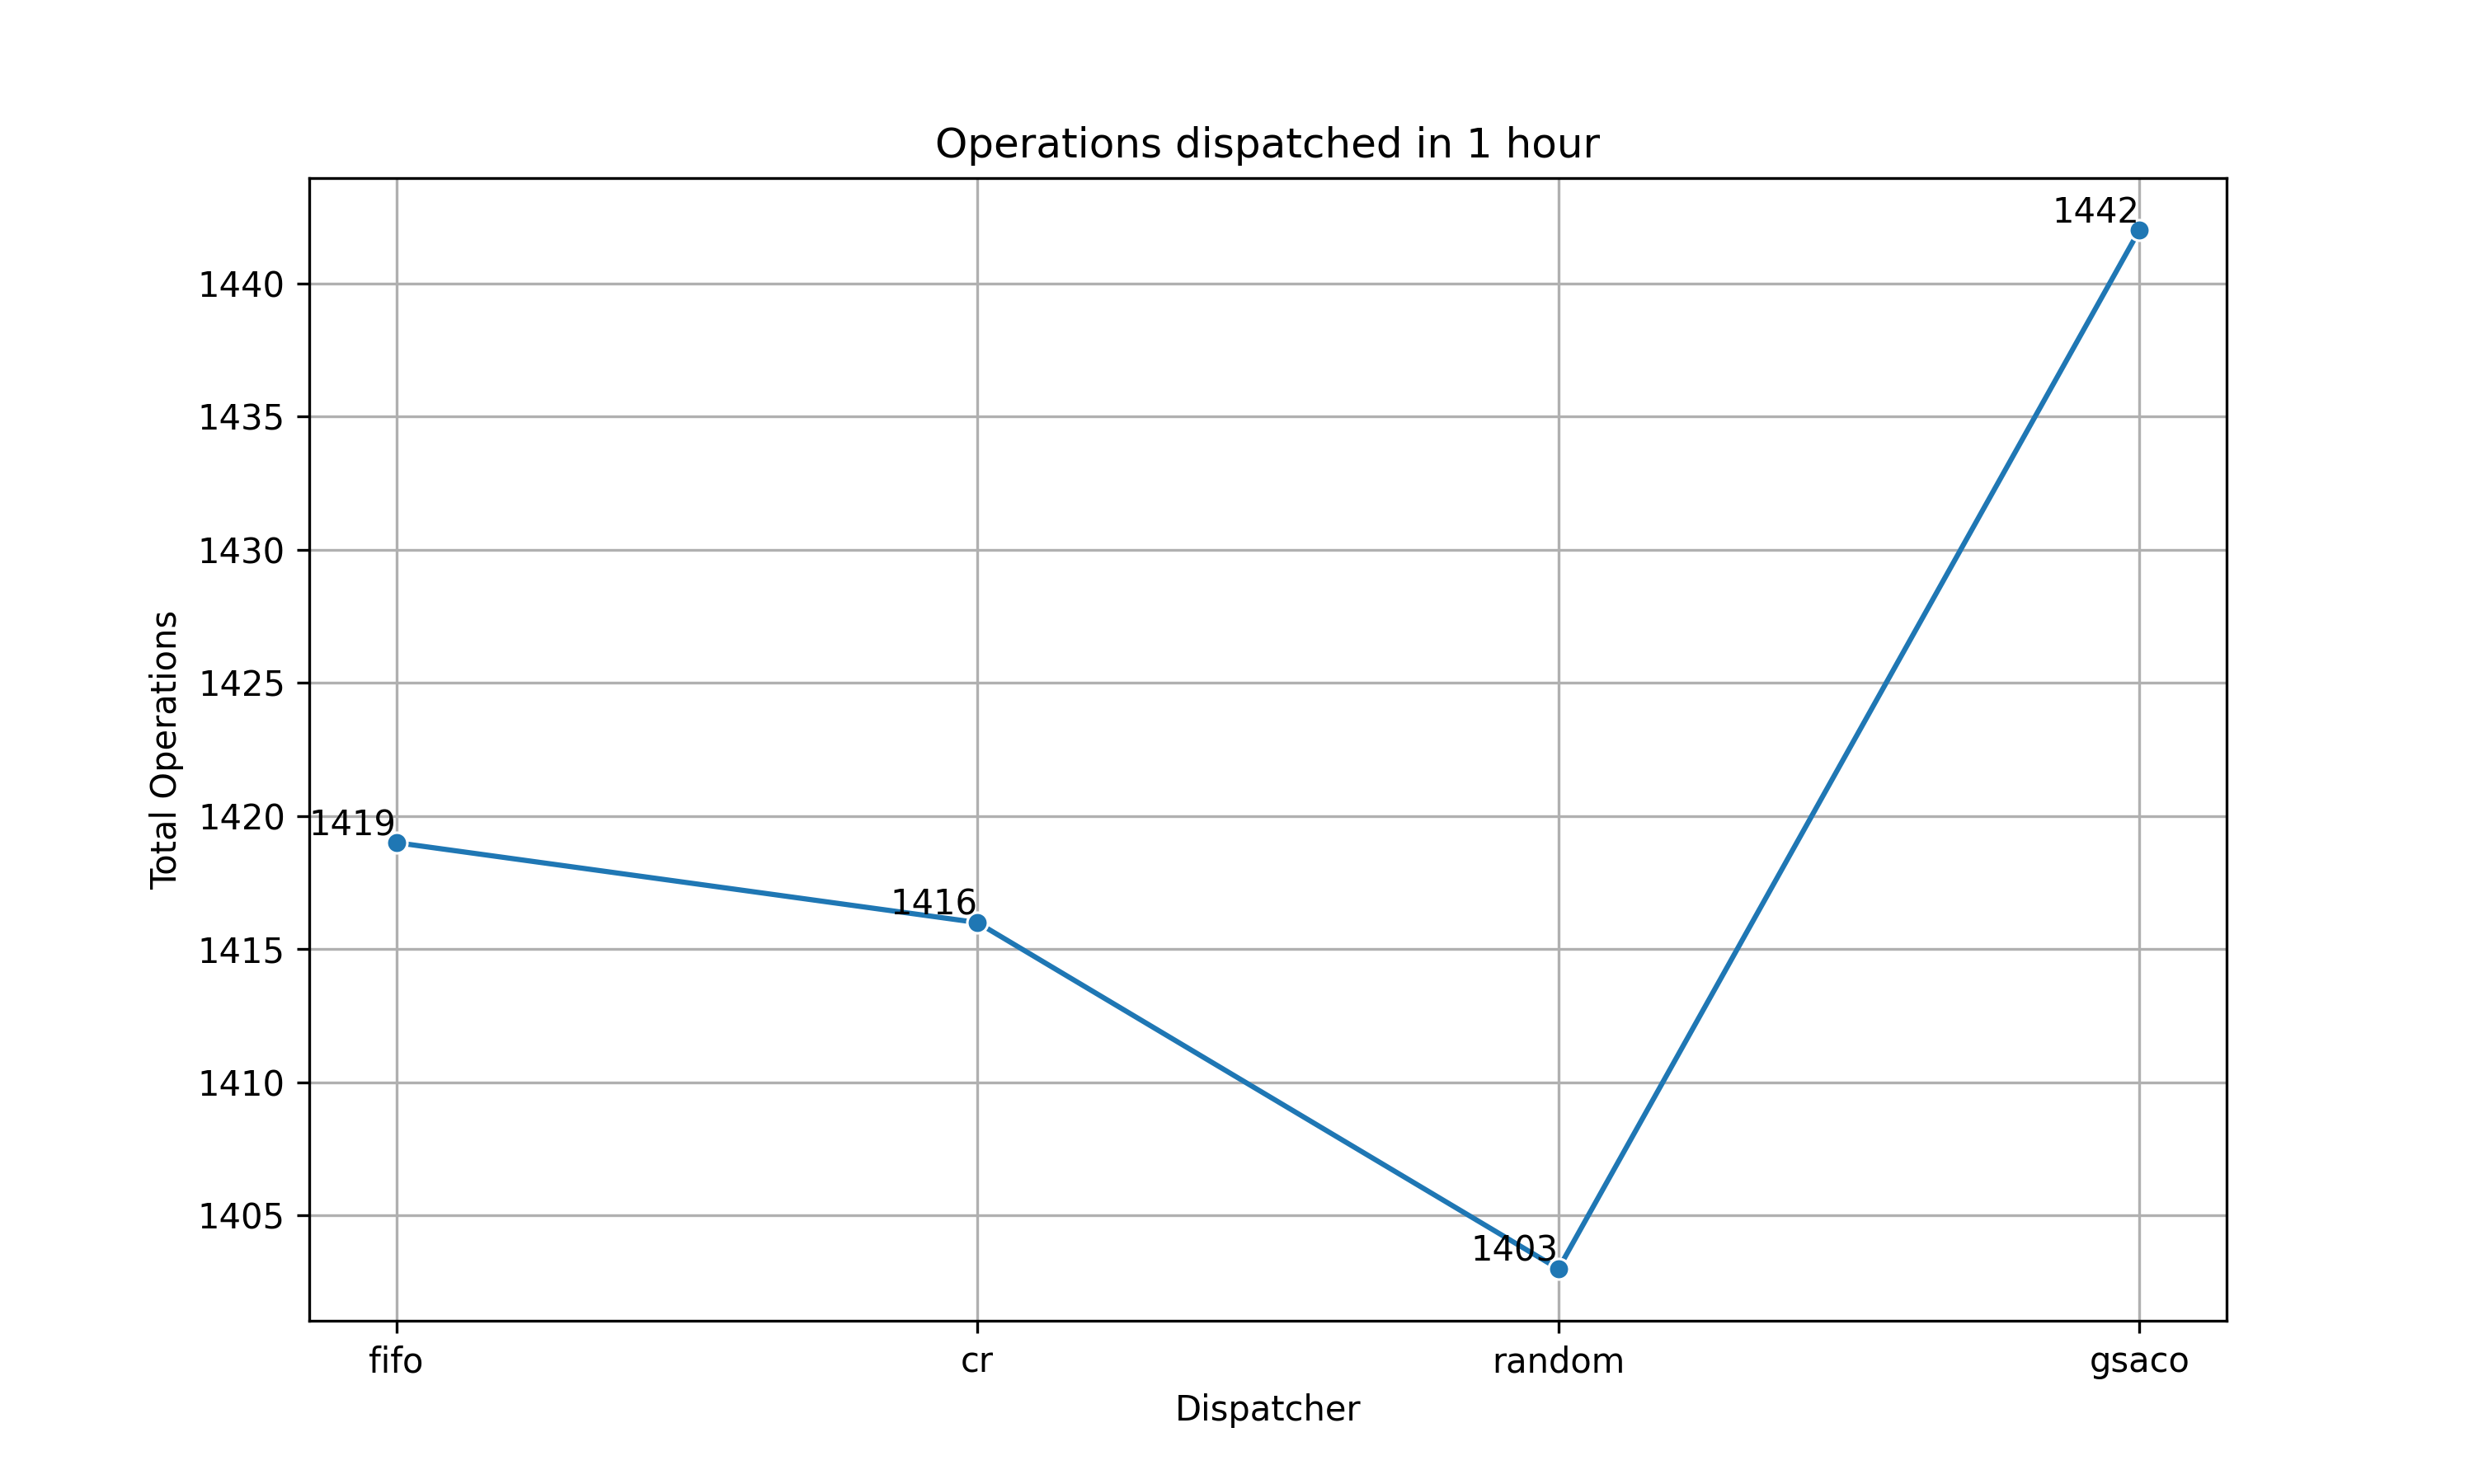
\includegraphics[width=\textwidth]{LVHM/total_operations_3600s.png}
		% \caption{}
		% \label{fig:oo1}
	\end{subfigure}\hfill
	\begin{subfigure}{0.32\textwidth}
		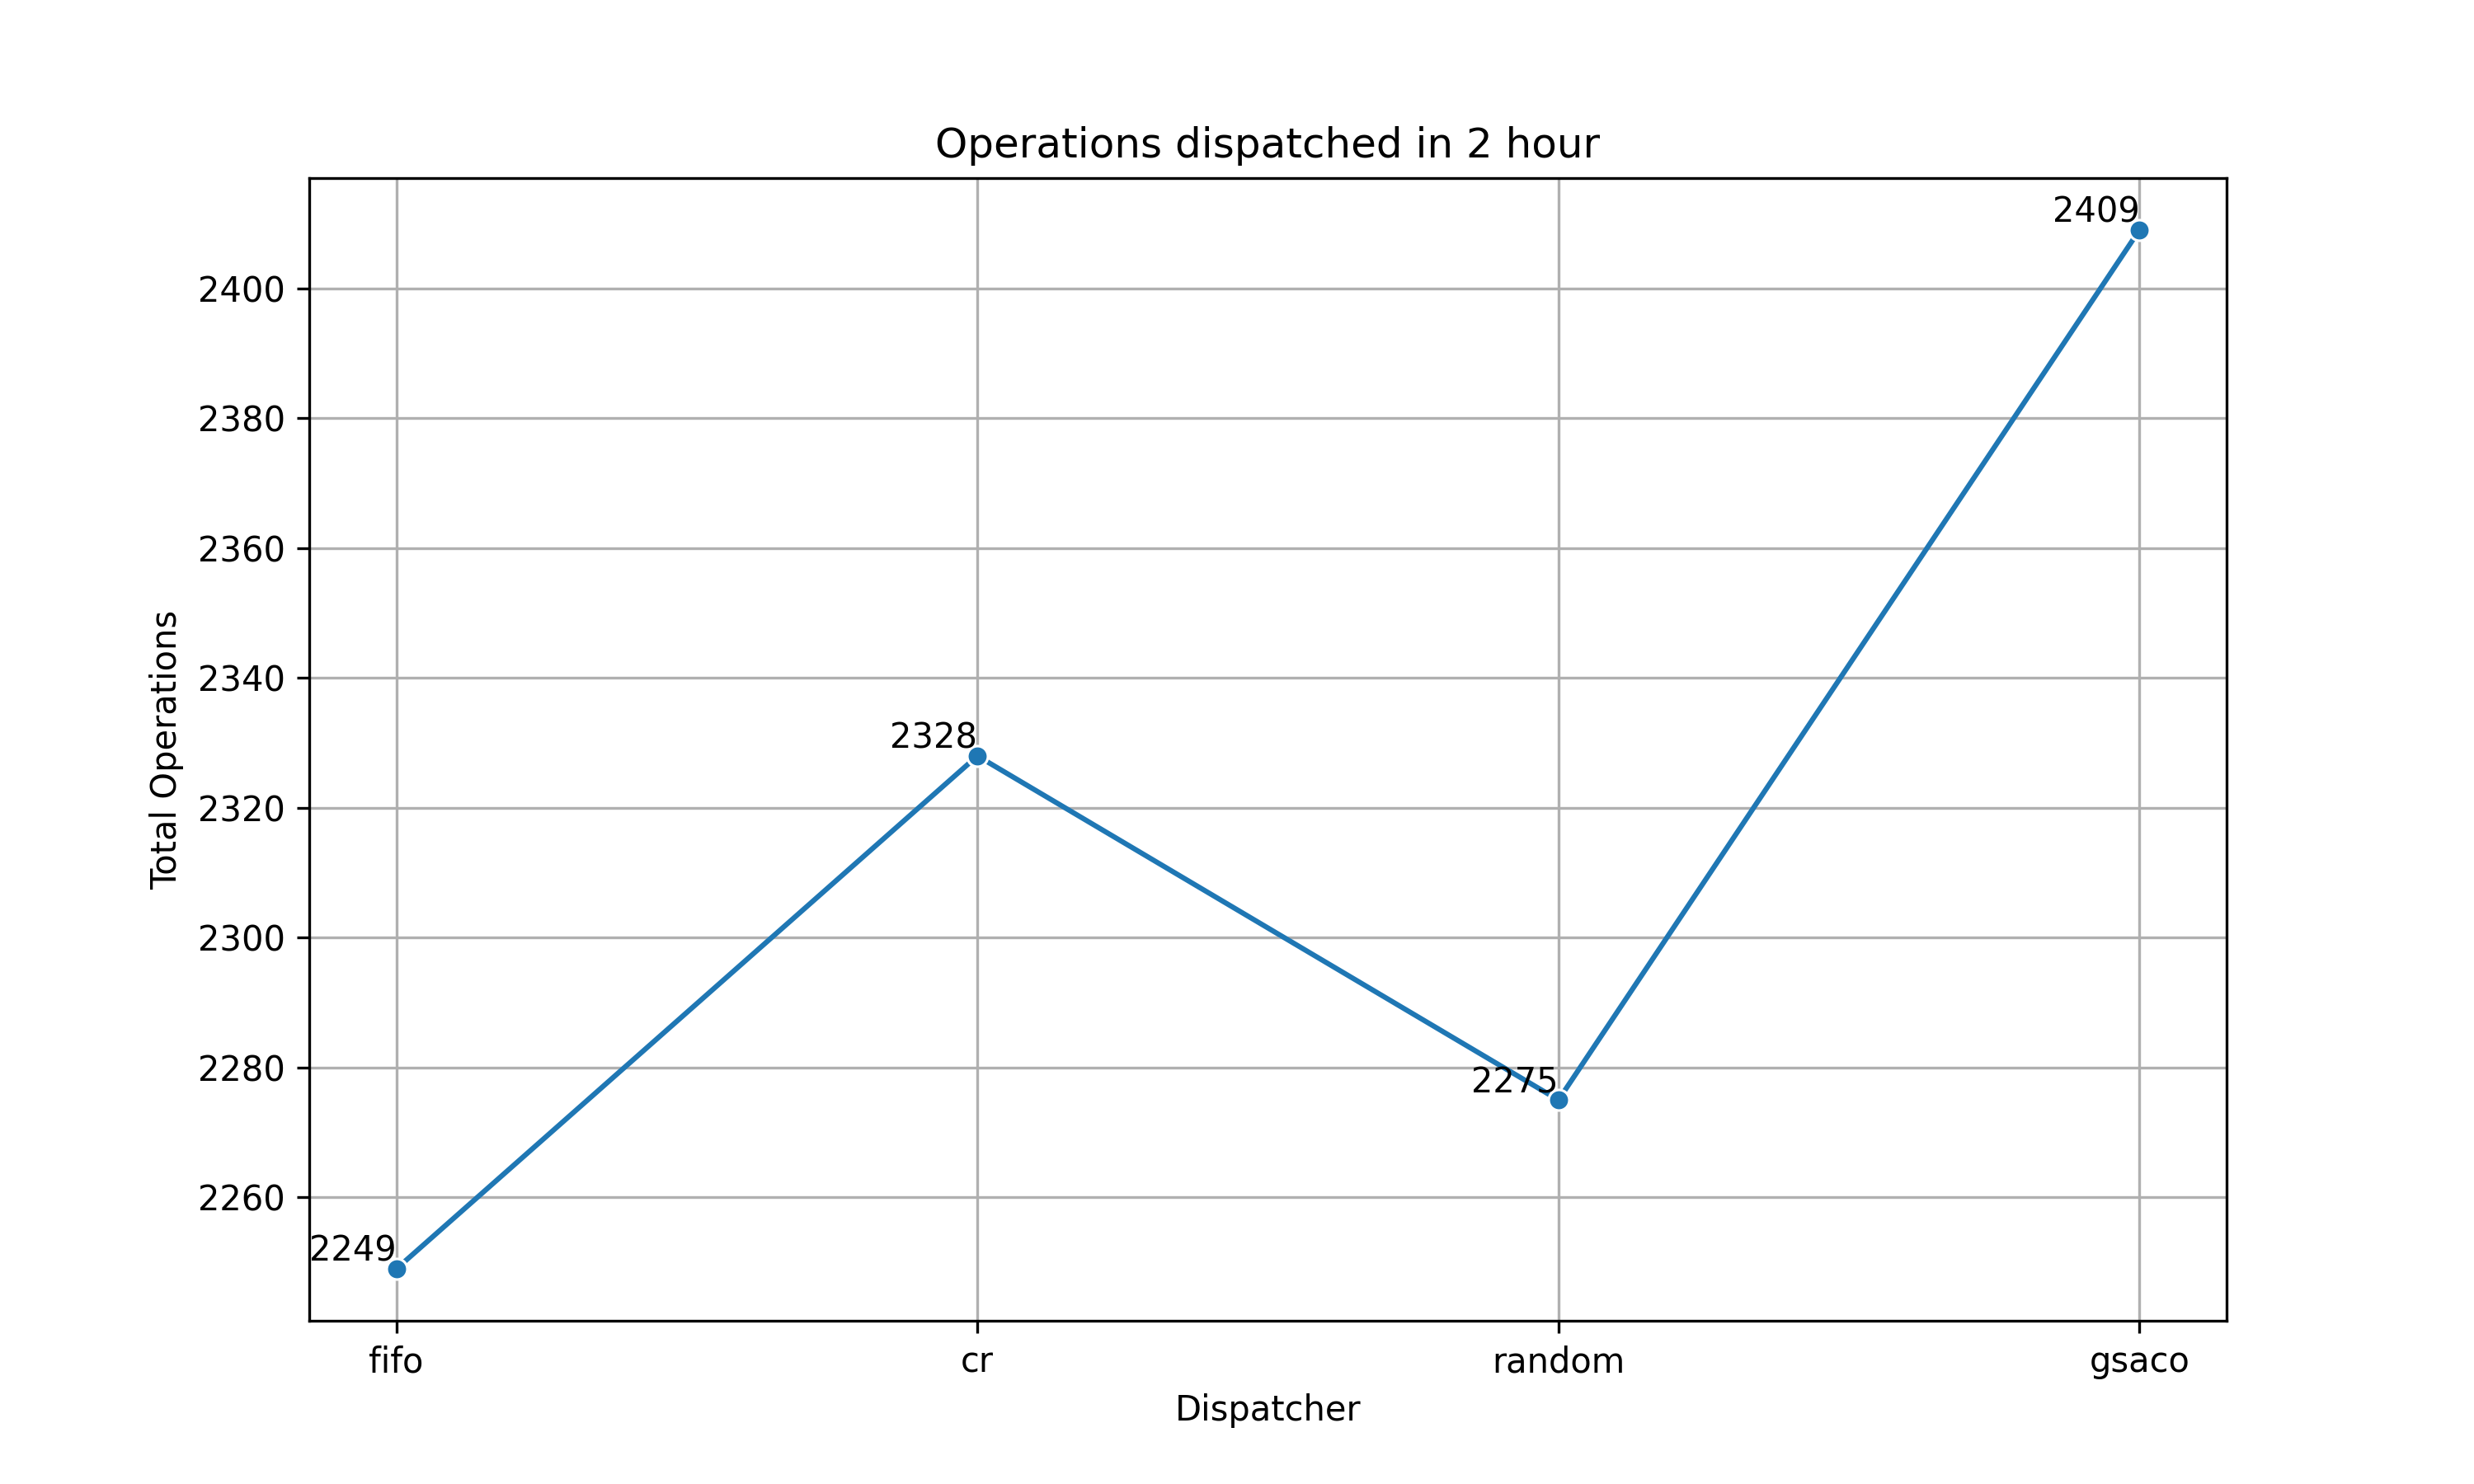
\includegraphics[width=\textwidth]{LVHM/total_operations_7200s.png}
		% \caption{}
		% \label{fig:oo2}
	\end{subfigure}\hfill
	\begin{subfigure}{0.32\textwidth}
		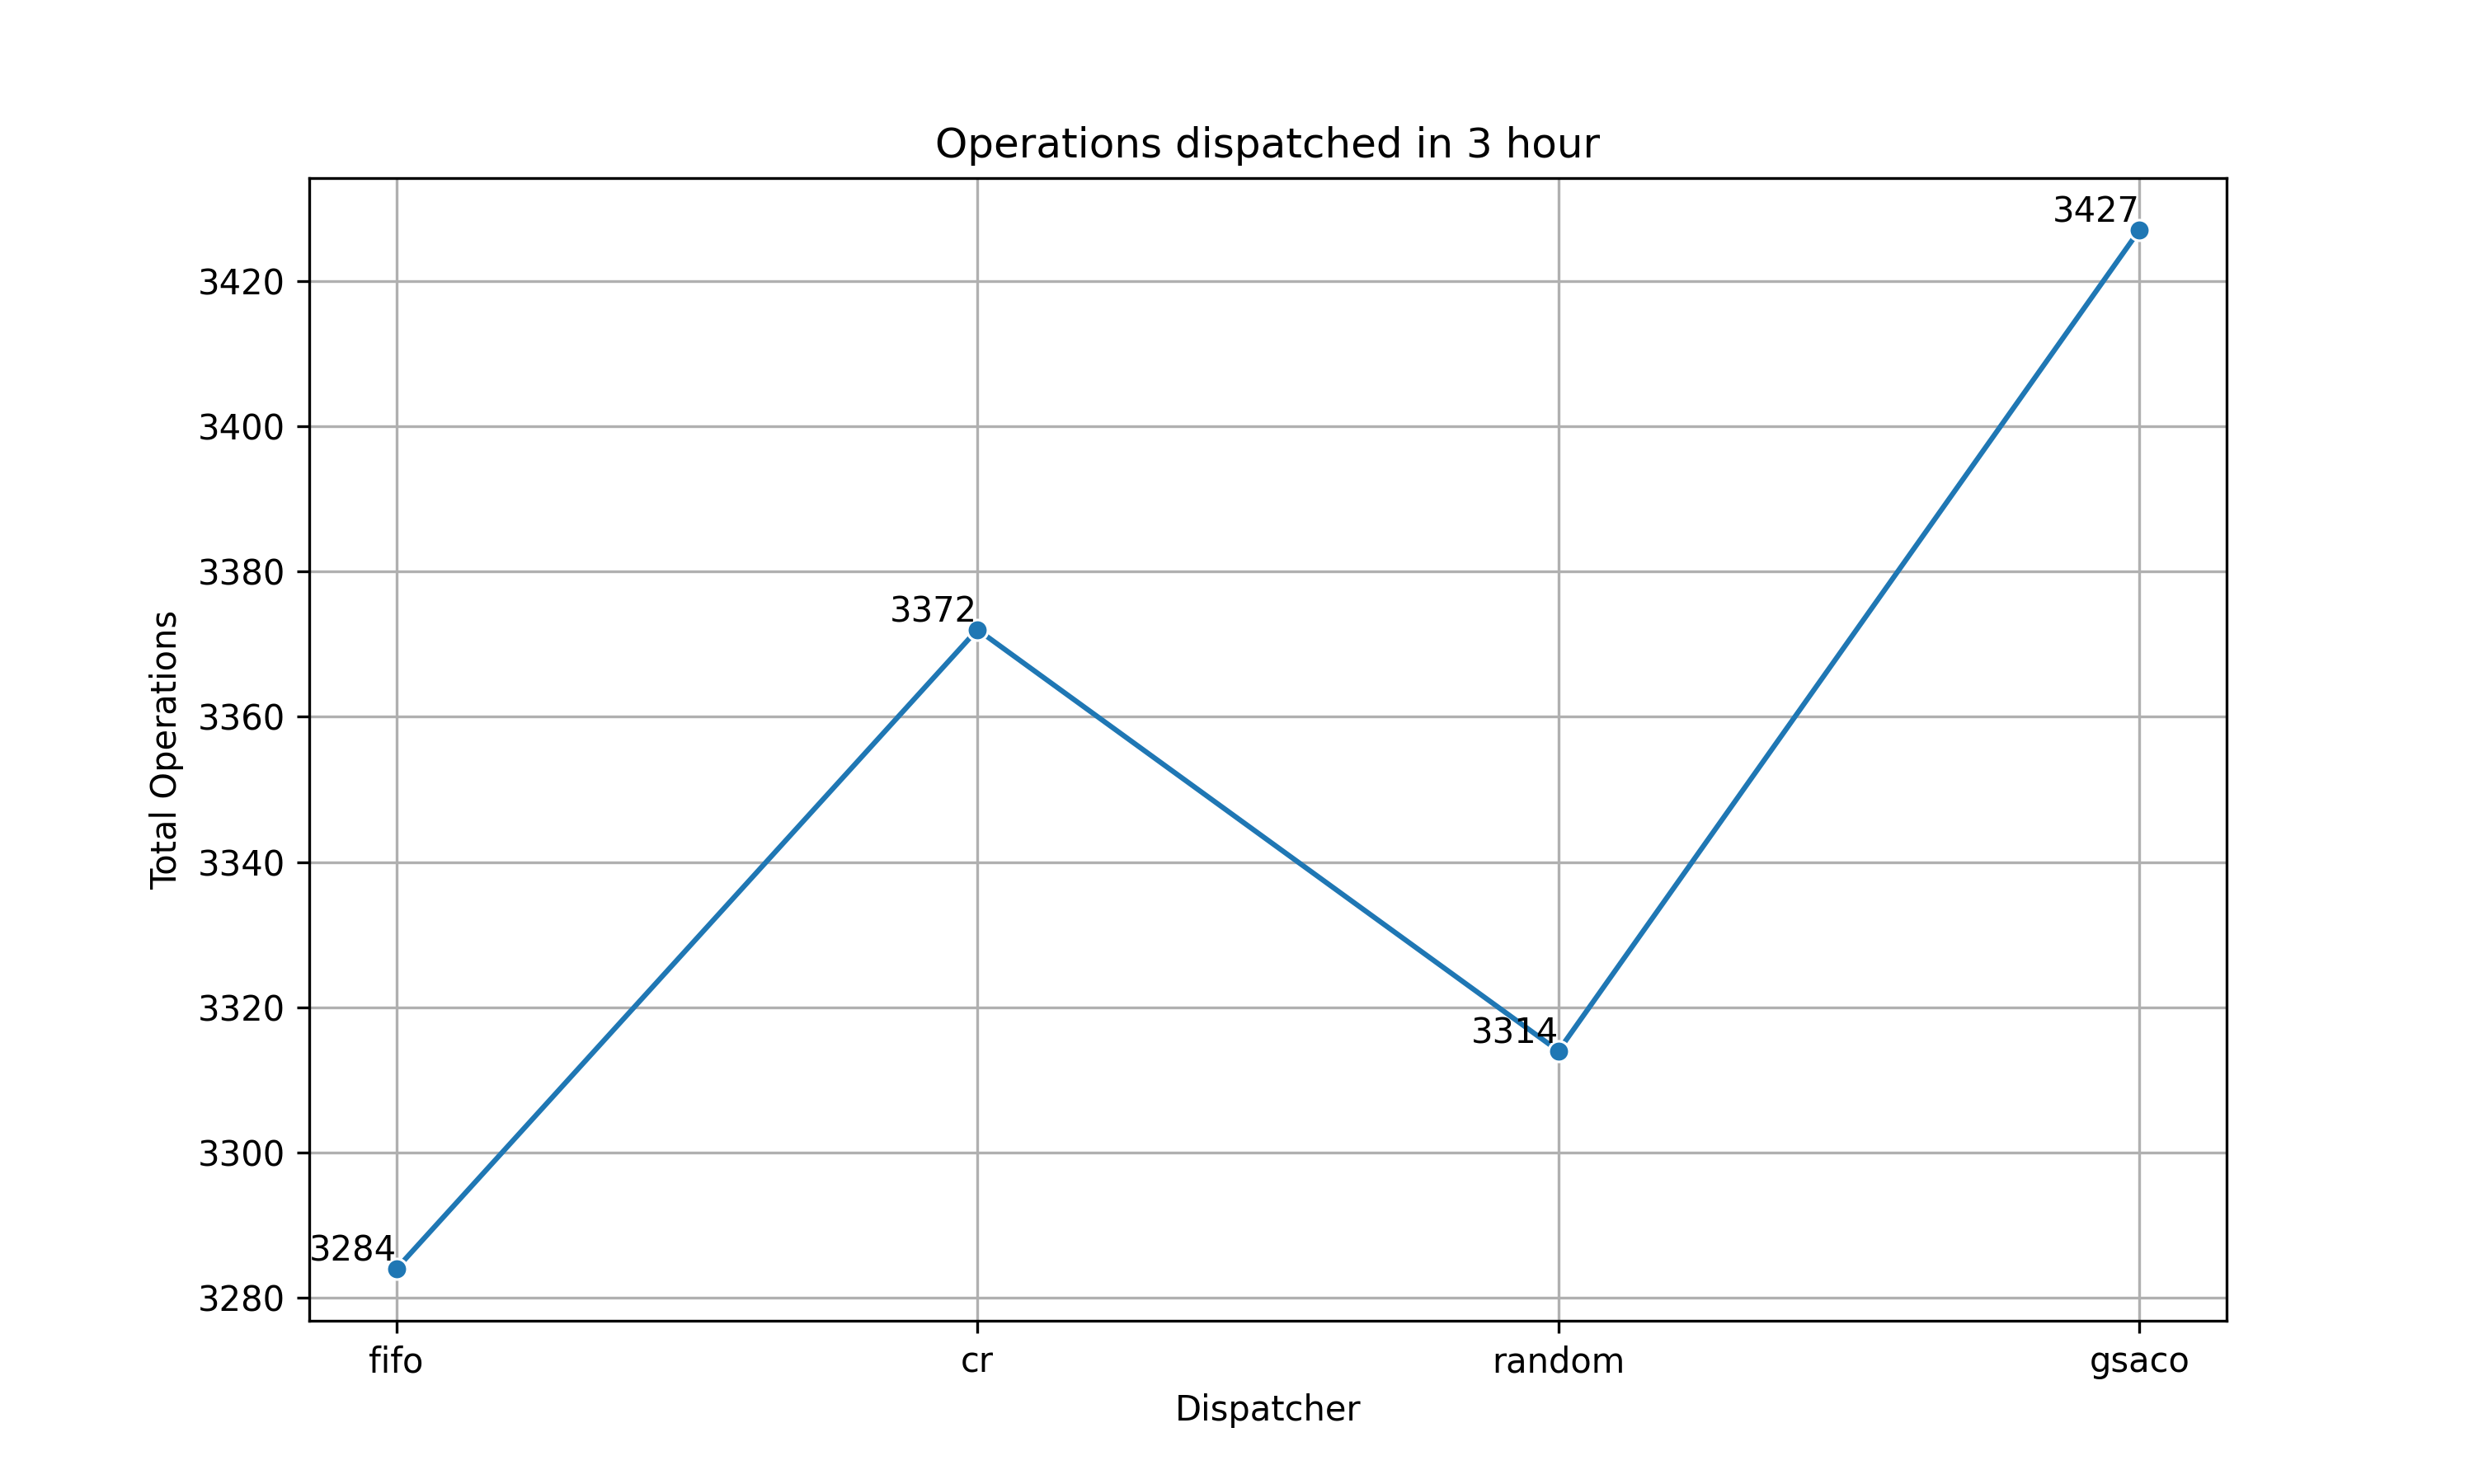
\includegraphics[width=\textwidth]{LVHM/total_operations_10800s.png}
		% \caption{}
		% \label{fig:oo3}
	\end{subfigure}
	\begin{subfigure}{0.32\textwidth}
		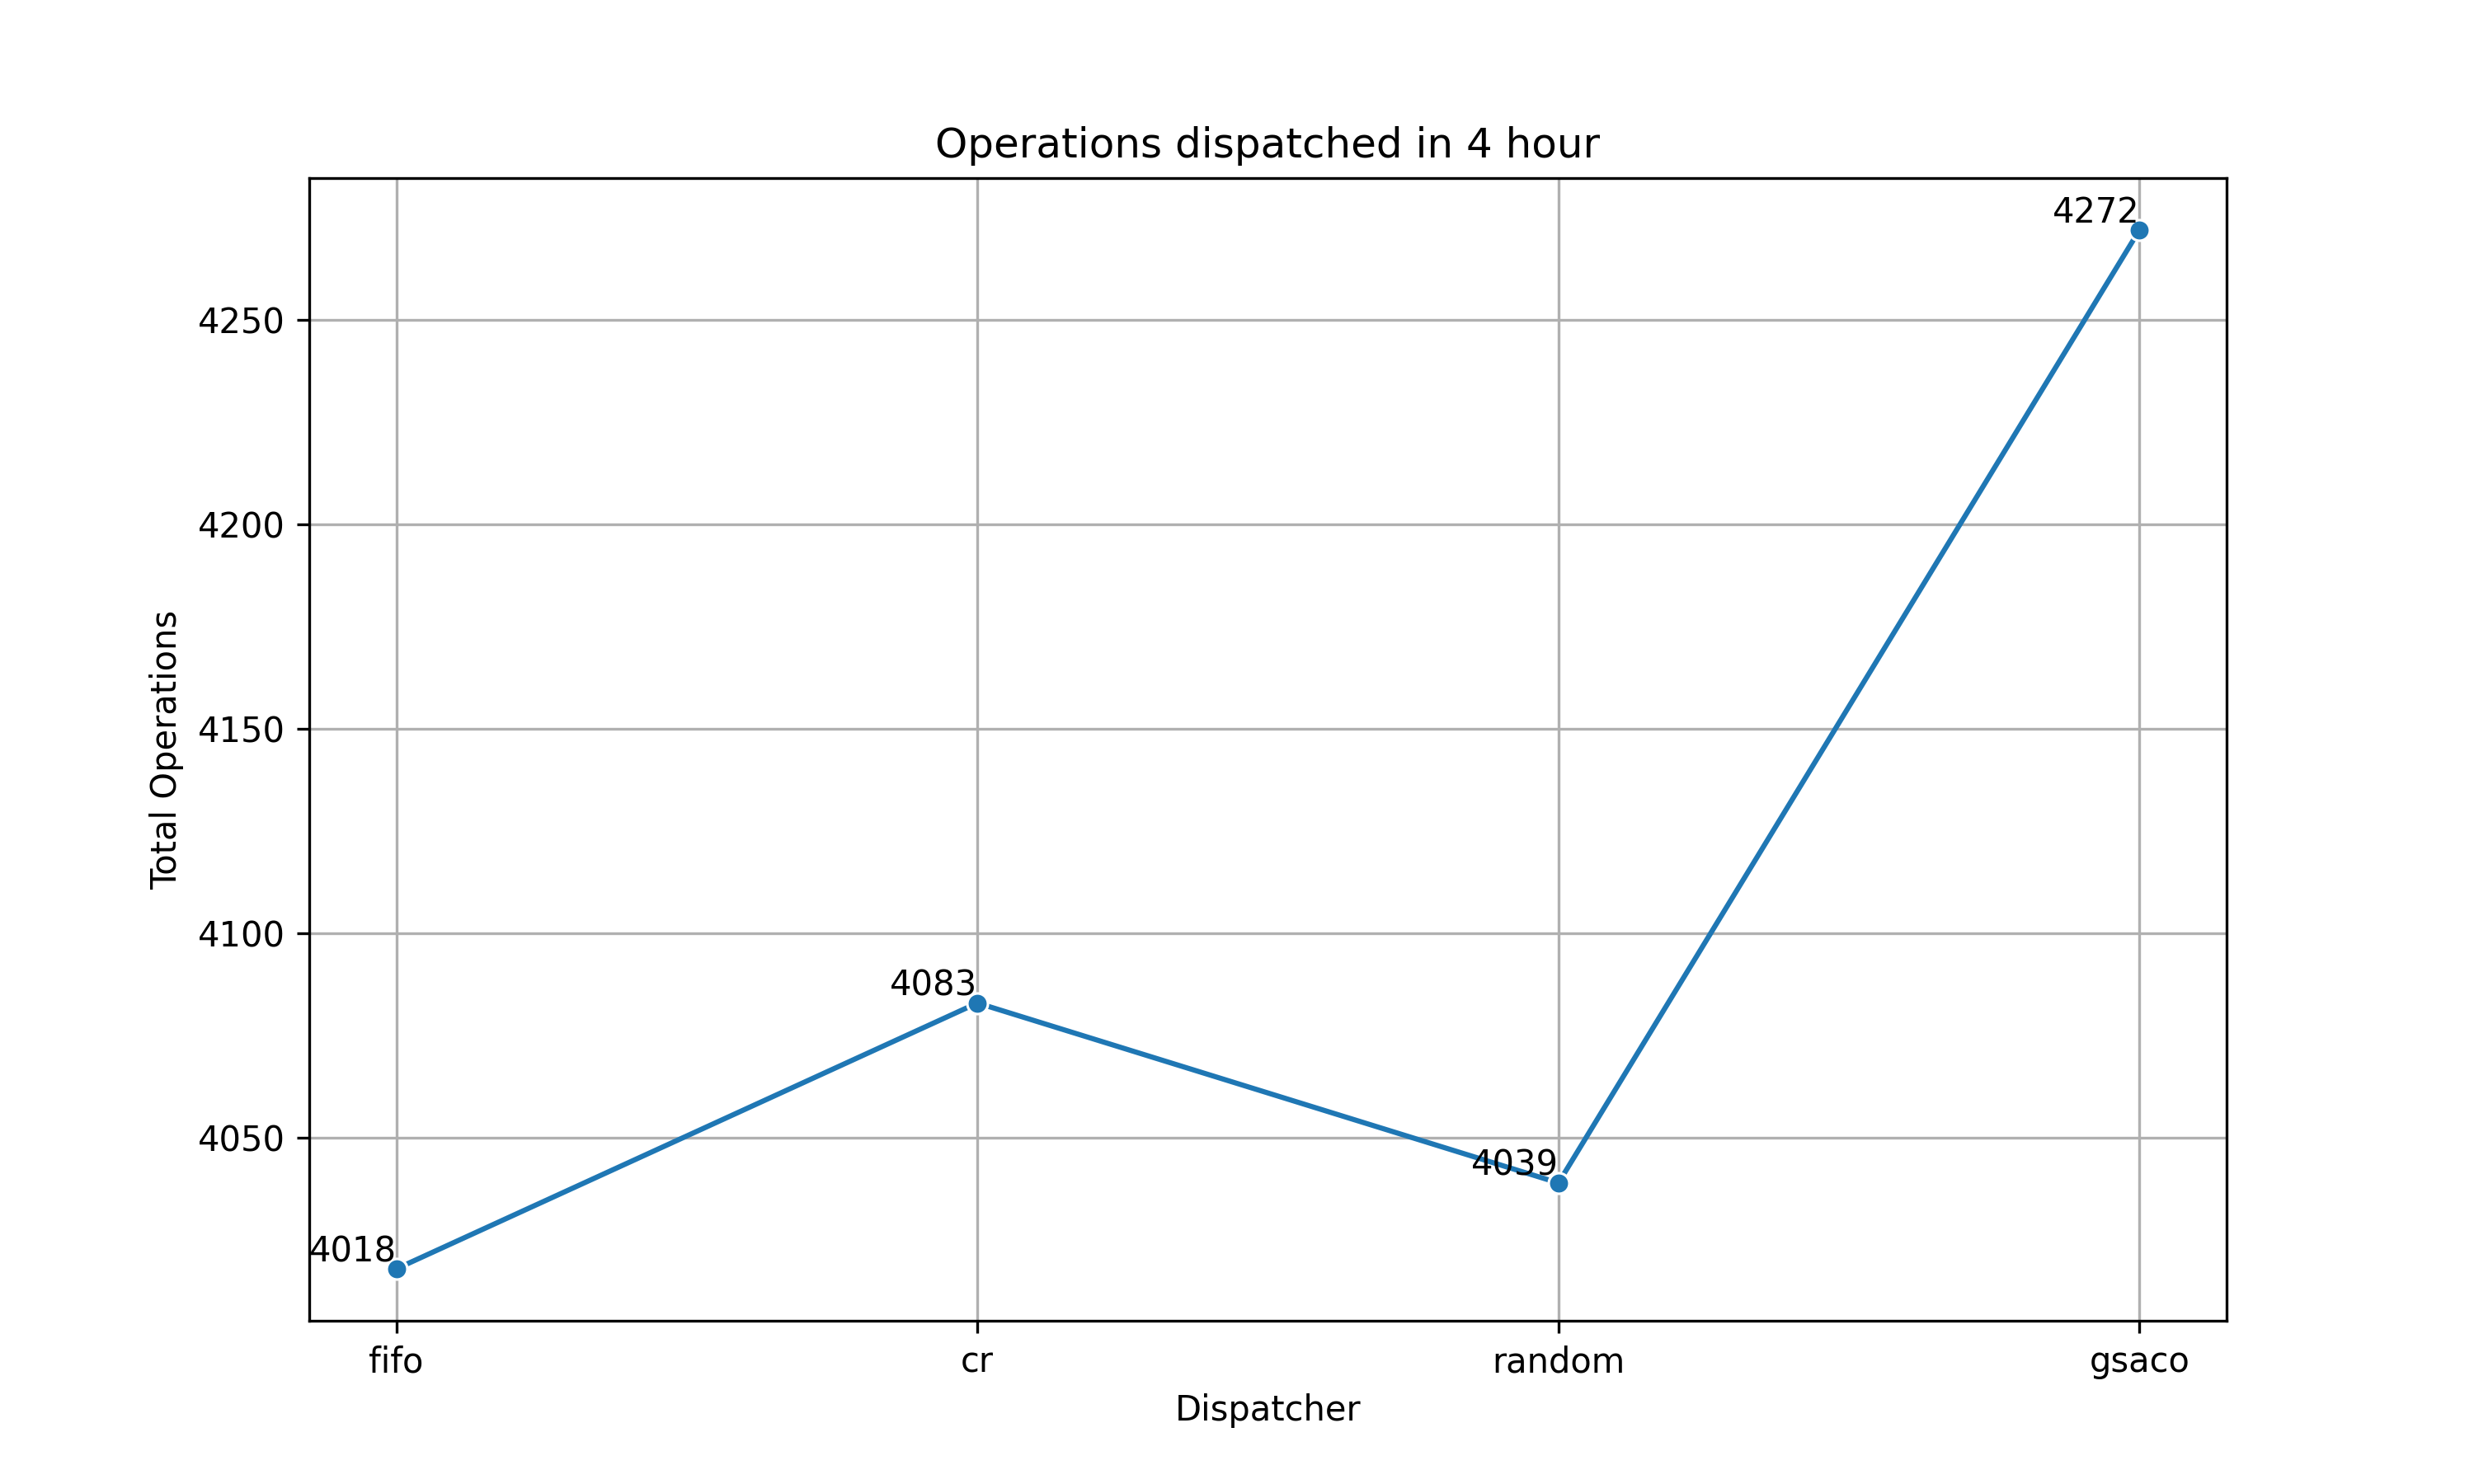
\includegraphics[width=\textwidth]{LVHM/total_operations_14400s.png}
		% \caption{}
		% \label{fig:oo4}
	\end{subfigure}\hfill
	\begin{subfigure}{0.32\textwidth}
		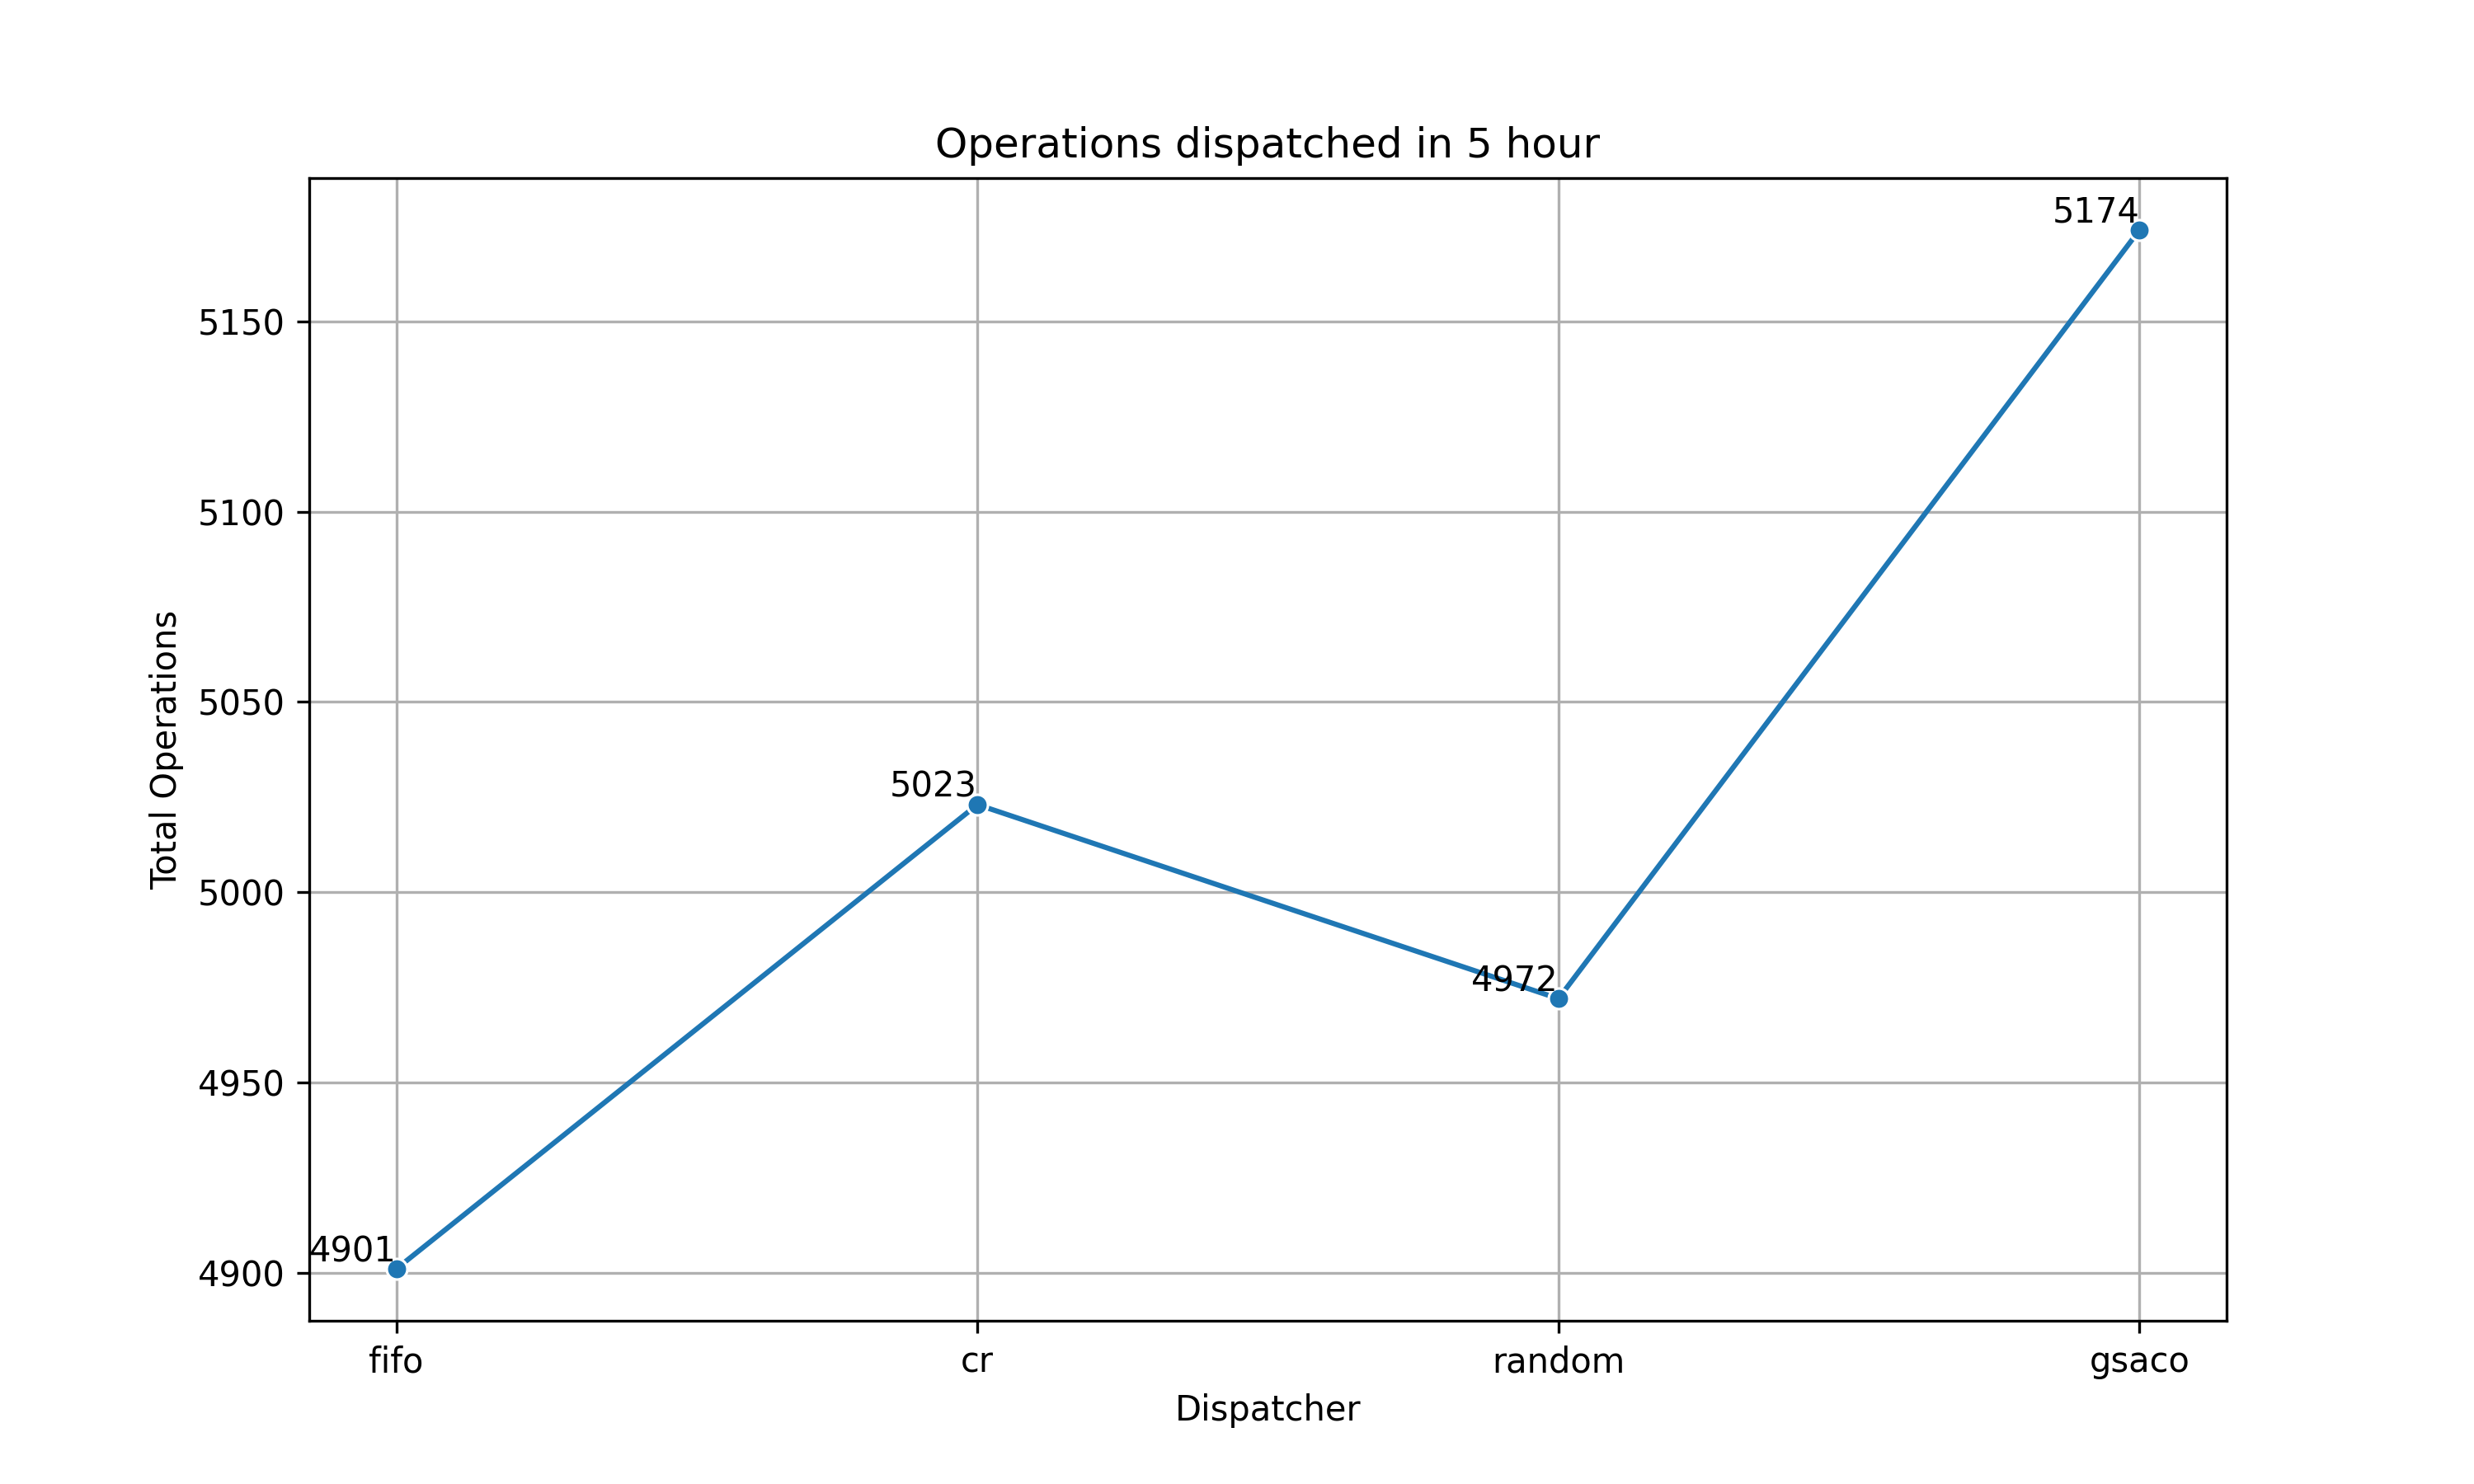
\includegraphics[width=\textwidth]{LVHM/total_operations_18000s.png}
		% \caption{}
		% \label{fig:oo5}
	\end{subfigure}\hfill
	\begin{subfigure}{0.32\textwidth}
		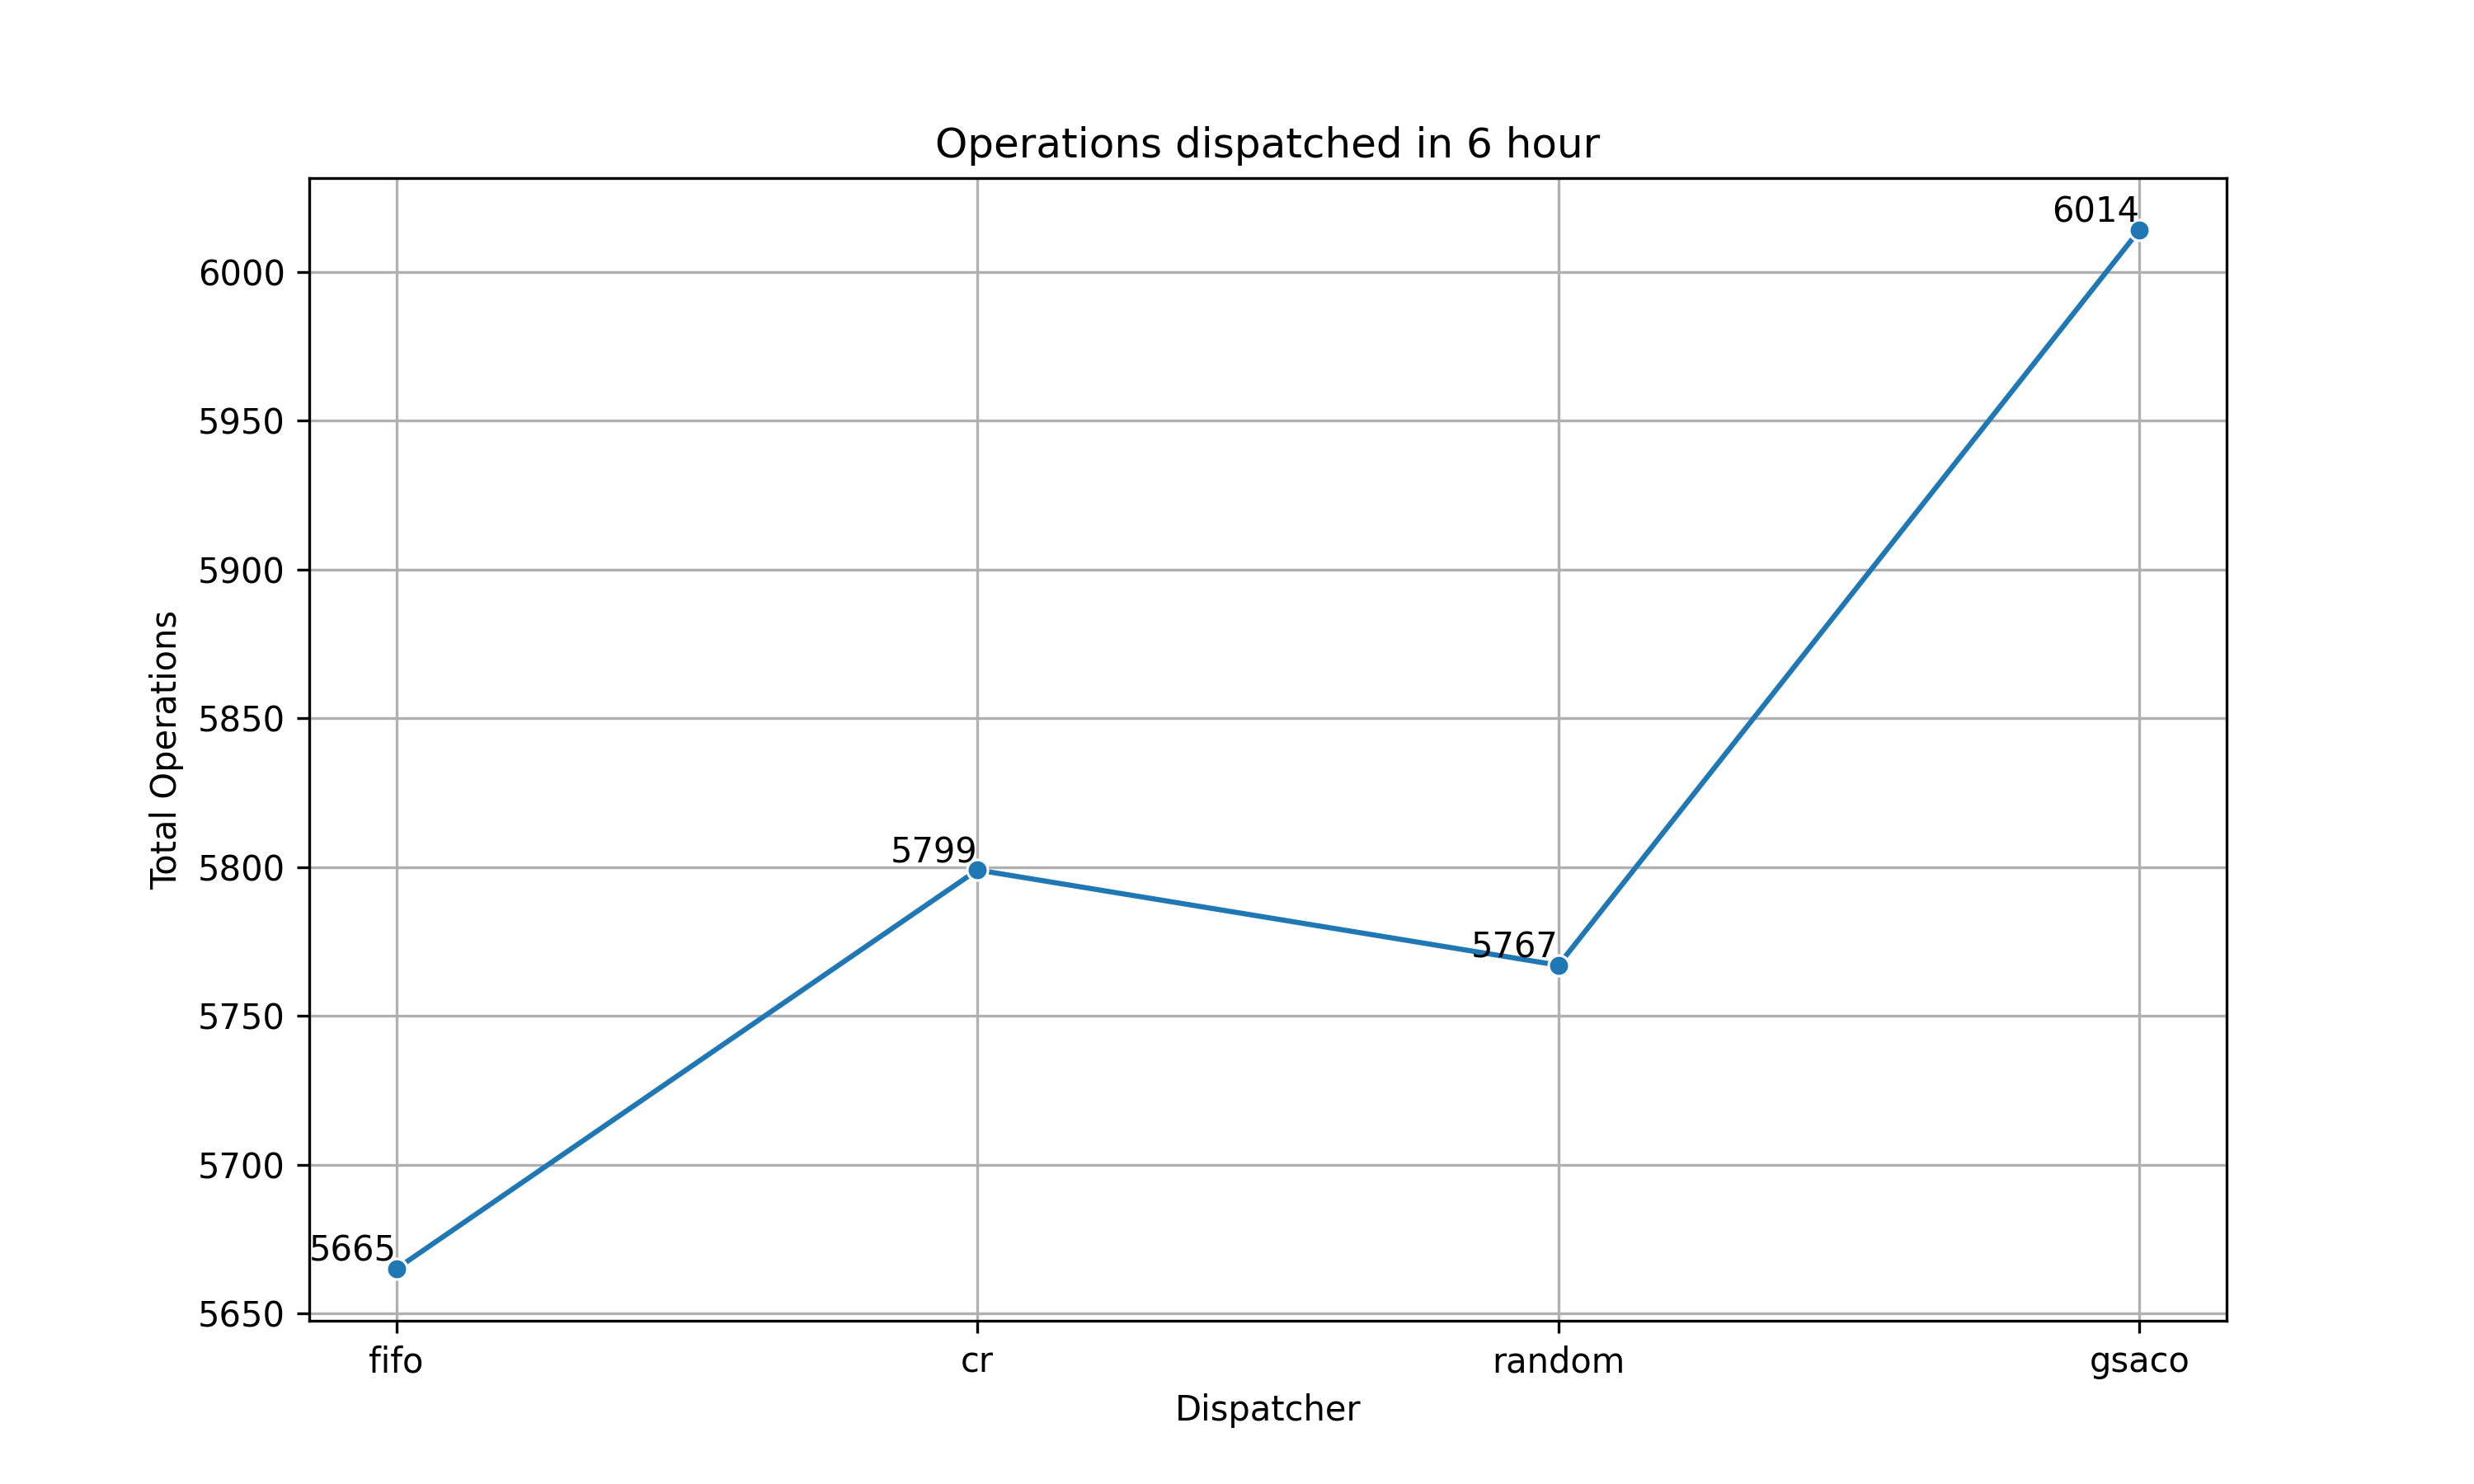
\includegraphics[width=\textwidth]{LVHM/total_operations_21600s.png}
		% \caption{}
		% \label{fig:oo6}
	\end{subfigure}
	\caption{Total operations completed LV/HM}
	\label{fig:totalopsLVHM}
\end{figure}